%!TEX program = xelatex
%!TEX options=--shell-escape
\documentclass[12pt]{article}

%
\usepackage[scheme=plain]{ctex}
%
\usepackage{fontspec}
%
\usepackage[margin = 1in]{geometry}

%
\usepackage[dvipsnames]{xcolor}
\usepackage[many]{tcolorbox}

%
\usepackage{amsmath}
\usepackage{amssymb}
\usepackage{amsthm}
%
\usepackage{tensor}
%
\usepackage{slashed}
\usepackage{physics}
\usepackage{simpler-wick}

%
\usepackage[version=4]{mhchem}

%
\usepackage{mathtools}

%
\usepackage{bm}
\newcommand{\dbar}{\dif\hspace*{-0.18em}\bar{}\hspace*{0.2em}}
\DeclareMathAlphabet\mathbfcal{OMS}{cmsy}{b}{n}
%\usepackage{bbold}
\newcommand*{\dif}{\mathop{}\!\mathrm{d}}
\newcommand*{\euler}{\mathrm{e}}
\newcommand*{\imagi}{\mathrm{i}}

\renewcommand{\vec}[1]{\boldsymbol{\mathbf{#1}}}

\usepackage{caption}

\usepackage{enumitem}

%
\usepackage{mathrsfs}
\usepackage{dsfont}

%
\usepackage{hyperref}
\hypersetup{
    colorlinks=true,
    linkcolor=violet,
    filecolor=blue,      
    urlcolor=blue,
    citecolor=cyan,
}

%
\usepackage{graphicx}
%
\graphicspath{{image/}}


%
\usepackage{indentfirst}
%
\setlength{\parindent}{2em}
\linespread{1.25}

% 
% \setmainfont{Times New Roman}

\title{Note}
\author{Feng-Yang Hsieh}
\date{}

\begin{document}
\maketitle
\section{Generate di-Higgs samples in SM}% (fold)
\label{sec:generate_di_higgs_samples_in_sm}
	Generate the double Higgs events in the standard model by MadGraph with \verb+loop_sm+ model. Following are the MadGraph scripts for generating di-Higgs samples:
	\begin{verbatim}
	import model loop_sm
	generate p p > h h [QCD] QED^2<=99 QCD^2<=99
	output /home/r10222035/CPVDM/Di-Higgs-SM/di-Higgs-sm

	launch /home/r10222035/CPVDM/Di-Higgs-SM/di-Higgs-sm

	shower=OFF
	detector=OFF
	analysis=OFF
	done

	set run_card nevents 10000
	set run_card ebeam1 6500.0
	set run_card ebeam2 6500.0

	done
	\end{verbatim}

	\subsection{Variation with \texorpdfstring{$\kappa_\lambda$}{kappa_lambda}}% (fold)
	\label{sub:variation_with_kappa_lambda}
		Reference: \href{https://answers.launchpad.net/mg5amcnlo/+question/678406}{How to change the trilinear Higgs coupling in Madgraph?}

		The definition of $\kappa_\lambda$
		\begin{equation}
			\kappa_\lambda \equiv \frac{\lambda_{HHH}}{\lambda_{HHH}^{\text{SM}}}
		\end{equation}

		Following the below steps, we can add a parameter $\kappa_\lambda$ in the model
		\begin{enumerate}
			\item Go to the MadGraph model file directory. Copy \verb+loop_sm+ to \verb+my_loop_sm+.
			\item Go to \verb+my_loop_sm+ directory. 
			\item In \verb+parameters.py+, add a new parameter for $\kappa_\lambda$ by
				\begin{verbatim}
				khhh = Parameter(name = 'khhh',
					  nature = 'external',
					  type = 'real',
					  value = 1,
					  texname = '\\text{khhh}',
					  lhablock = 'SMINPUTS',
					  lhacode = [ 10 ])
				\end{verbatim}
			\item In \verb+vertices.py+, we can find the coupling for three Higgs vertex in the form \verb+GC_XX+. 
			\item In \verb+couplings.py+, multiply the value for \verb+GC_XX+ found in step 4 by \verb+khhh+.
			\item In \verb+restrict_default.dat+, add
				\begin{verbatim}
				10 2.000000e+00 # khhh 
				\end{verbatim}
				in Block SMINPUTS.
		\end{enumerate}

		Finish the above setting we can use the following scripts to generate di-Higgs samples:
			\begin{verbatim}
			import model my_loop_sm
			generate p p > h h [QCD] QED^2<=99 QCD^2<=99
			output /home/r10222035/CPVDM/Di-Higgs-SM/di-Higgs-sm-kappa

			launch /home/r10222035/CPVDM/Di-Higgs-SM/di-Higgs-sm-kappa

			shower=OFF
			detector=OFF
			analysis=OFF
			done

			set param_card khhh 1

			set run_card nevents 10000
			set run_card ebeam1 6500.0
			set run_card ebeam2 6500.0

			done
			\end{verbatim}

	% subsection variation_with_kappa_lambda (end)
	\subsection{Results}% (fold)
	\label{sub:di_Higgs_sample_generating_results}
		The cross sections of various $\kappa_\lambda$ are shown in Table \ref{tab:di-Higgs-SM-kappa-cross-section}.
		\begin{table}[htpb]
			\centering
			\caption{The cross sections of various $\kappa_\lambda$. My data is the results from MadGraph. The reference data is from \href{https://link.springer.com/content/pdf/10.1007/JHEP06(2019)066.pdf}{here}. }
			\label{tab:di-Higgs-SM-kappa-cross-section}
			\begin{tabular}{c|cc|c|cc|cc|c}
							 & \multicolumn{3}{c|}{13 TeV}                     & \multicolumn{5}{c}{14 TeV}                                     \\
							 & \multicolumn{2}{c|}{Cross section (fb)} &        & \multicolumn{2}{c|}{Cross section (fb)} &       &               \\
							 $\kappa_\lambda$ & Ref.              & My data            & Ref./My& Ref.              & My data            &Ref./My& Ref. K& Ref.K/My K \\ \hline
			-1               & 116.71            & 74.62              & 1.564  & 136.91            & 87.93              & 1.56 & 1.86 & 1.19  \\
			0                & 62.51             & 41.96              & 1.490  & 73.64             & 49.45              & 1.49 & 1.79 & 1.20  \\
			1                & 27.84             & 20.27              & 1.373  & 32.88             & 24.05              & 1.37 & 1.66 & 1.21  \\
			2                & 12.42             & 9.56               & 1.299  & 14.75             & 11.34              & 1.30 & 1.56 & 1.20  \\
			2.4              & 11.65             & 8.33               & 1.399  & 13.79             & 9.90               & 1.39 & 1.65 & 1.18  \\
			3                & 16.28             & 9.81               & 1.660  & 19.07             & 11.55              & 1.65 & 1.90 & 1.15  \\
			5                & 81.74             & 43.55              & 1.877  & 95.22             & 50.68              & 1.88 & 2.14 & 1.14  \\
			\end{tabular}
		\end{table}

		The $m_{HH}$ distribution with various $\kappa_\lambda$ is presented in Figure \ref{fig:di-Higgs-SM-kappa-mhh}. In the left plot, the data is the parton level data from MadGraph. The right plot comes from the ATLAS reference. Here, the $\sqrt{s} = \text{13 TeV}$
		\begin{figure}[htpb]
			\centering
			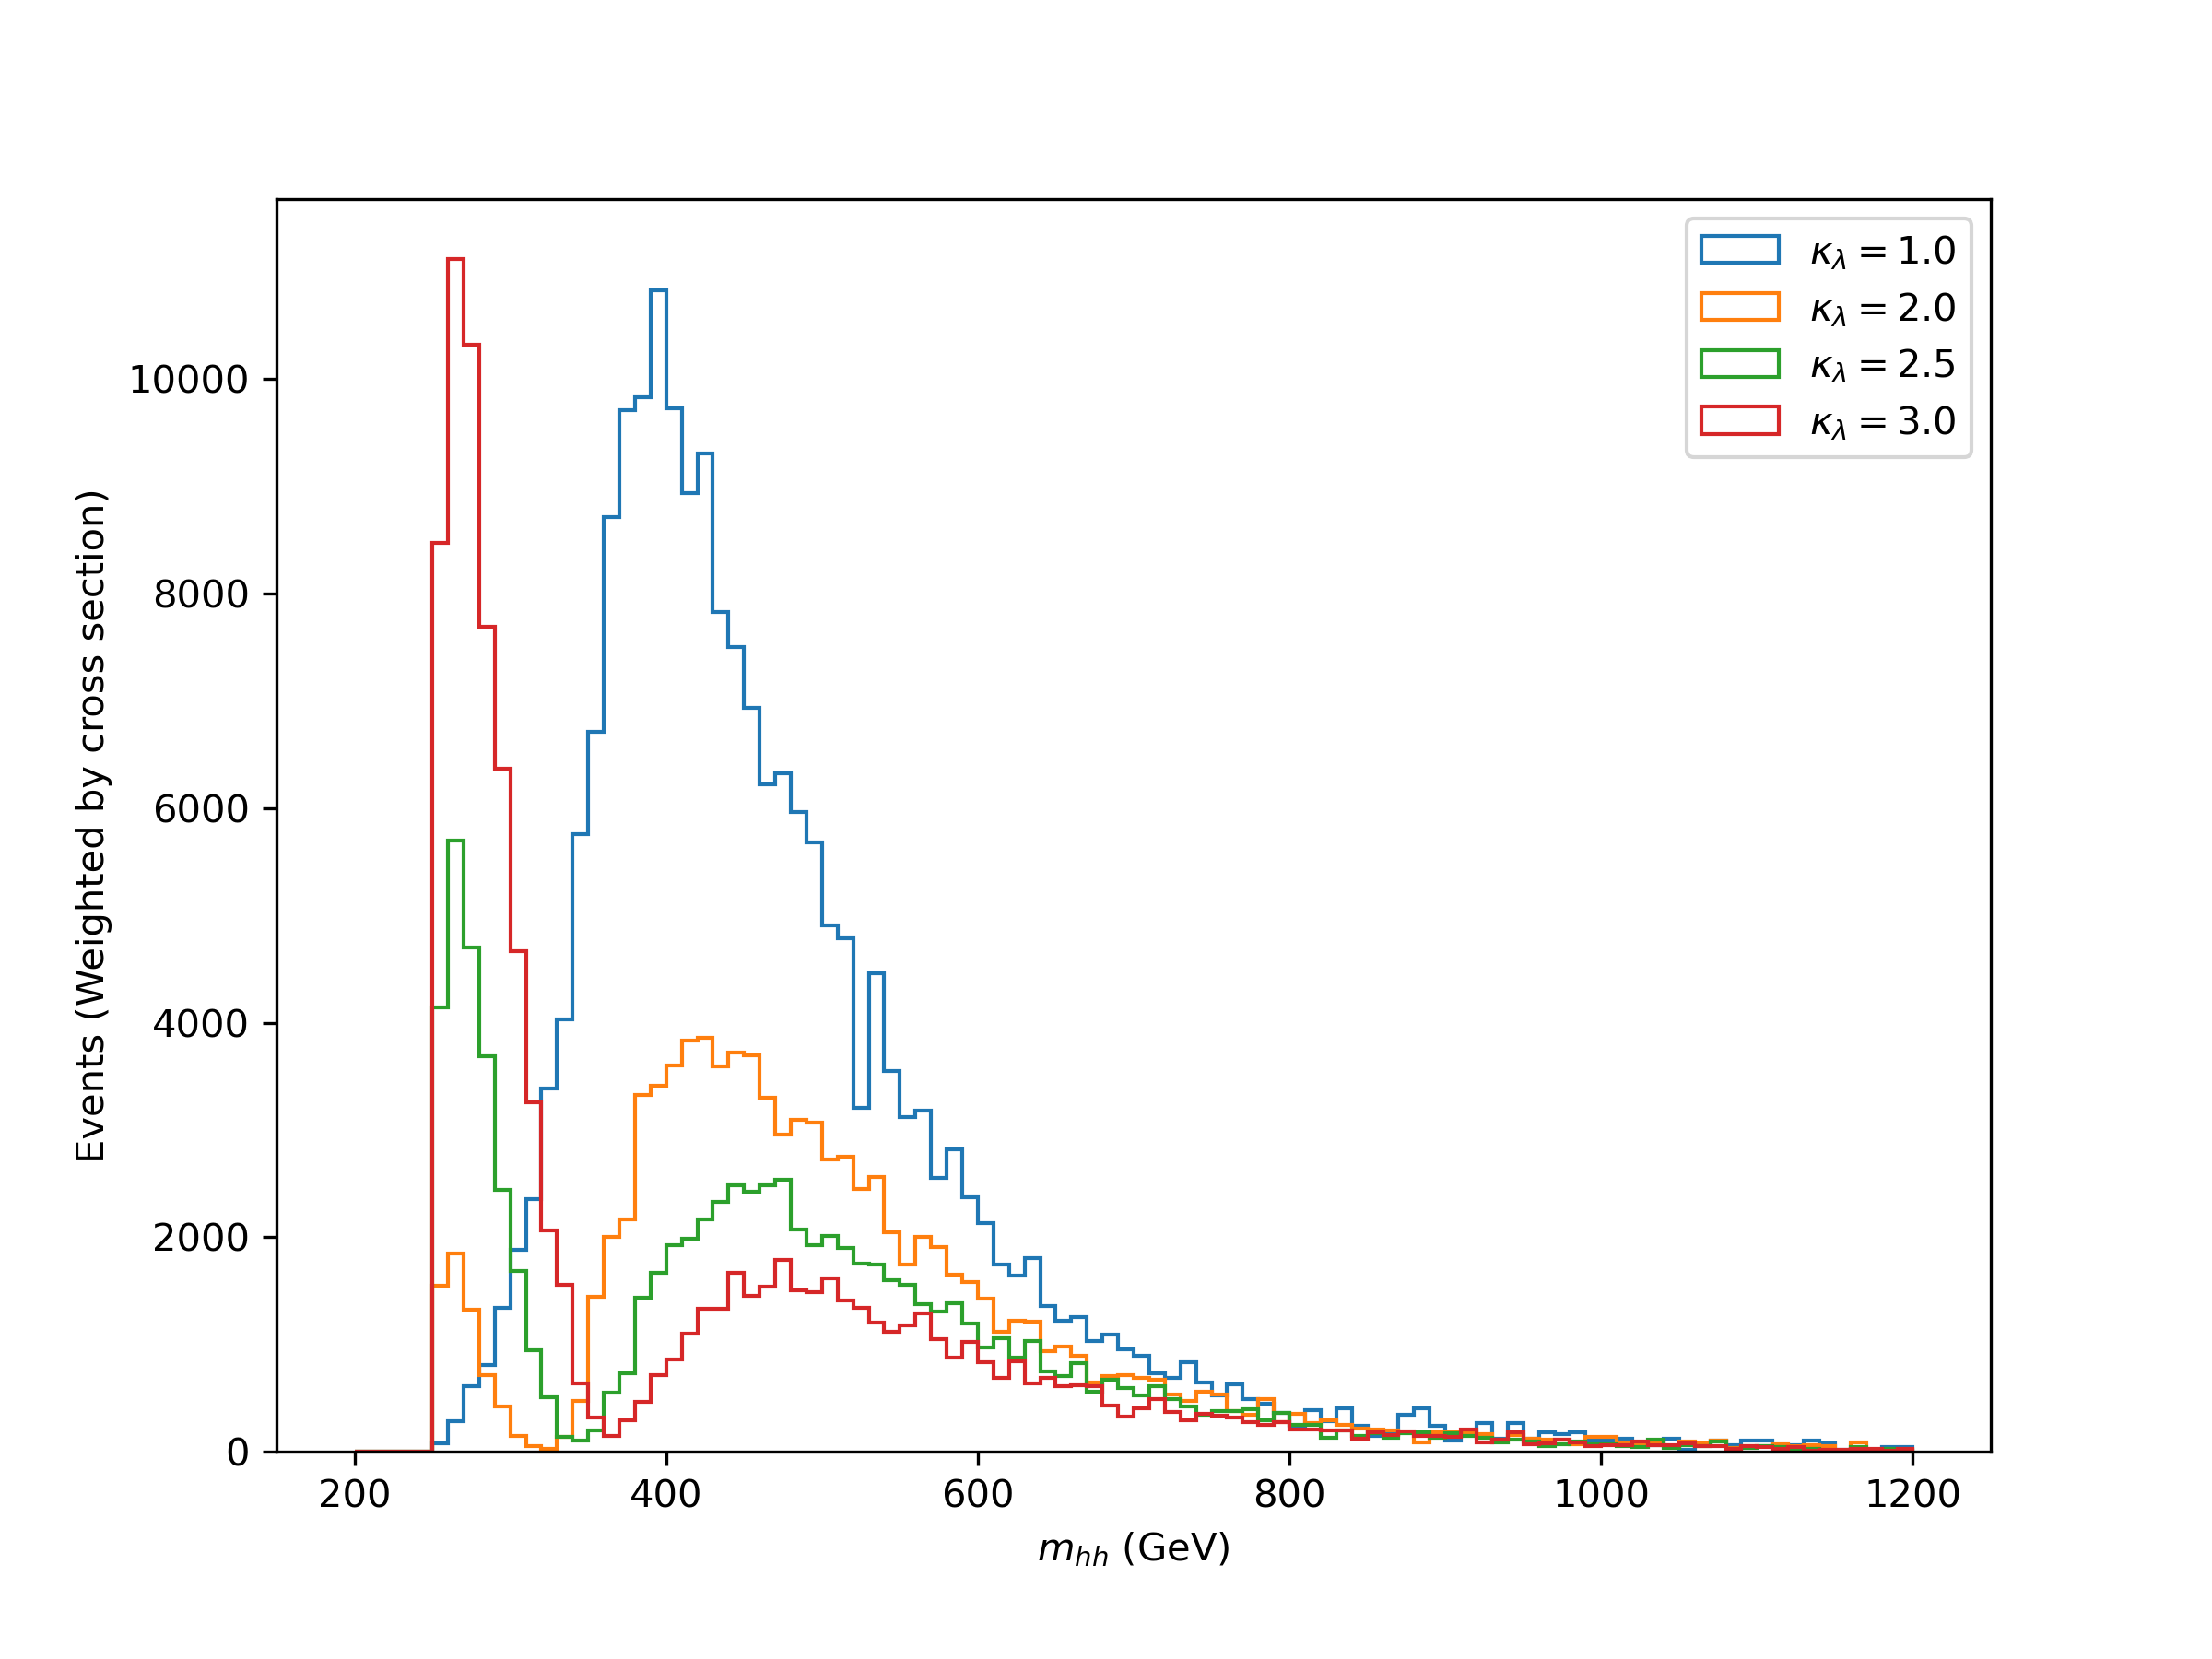
\includegraphics[width=0.49\textwidth]{di-Higgs-SM-kappa-mhh-my-data.png}
			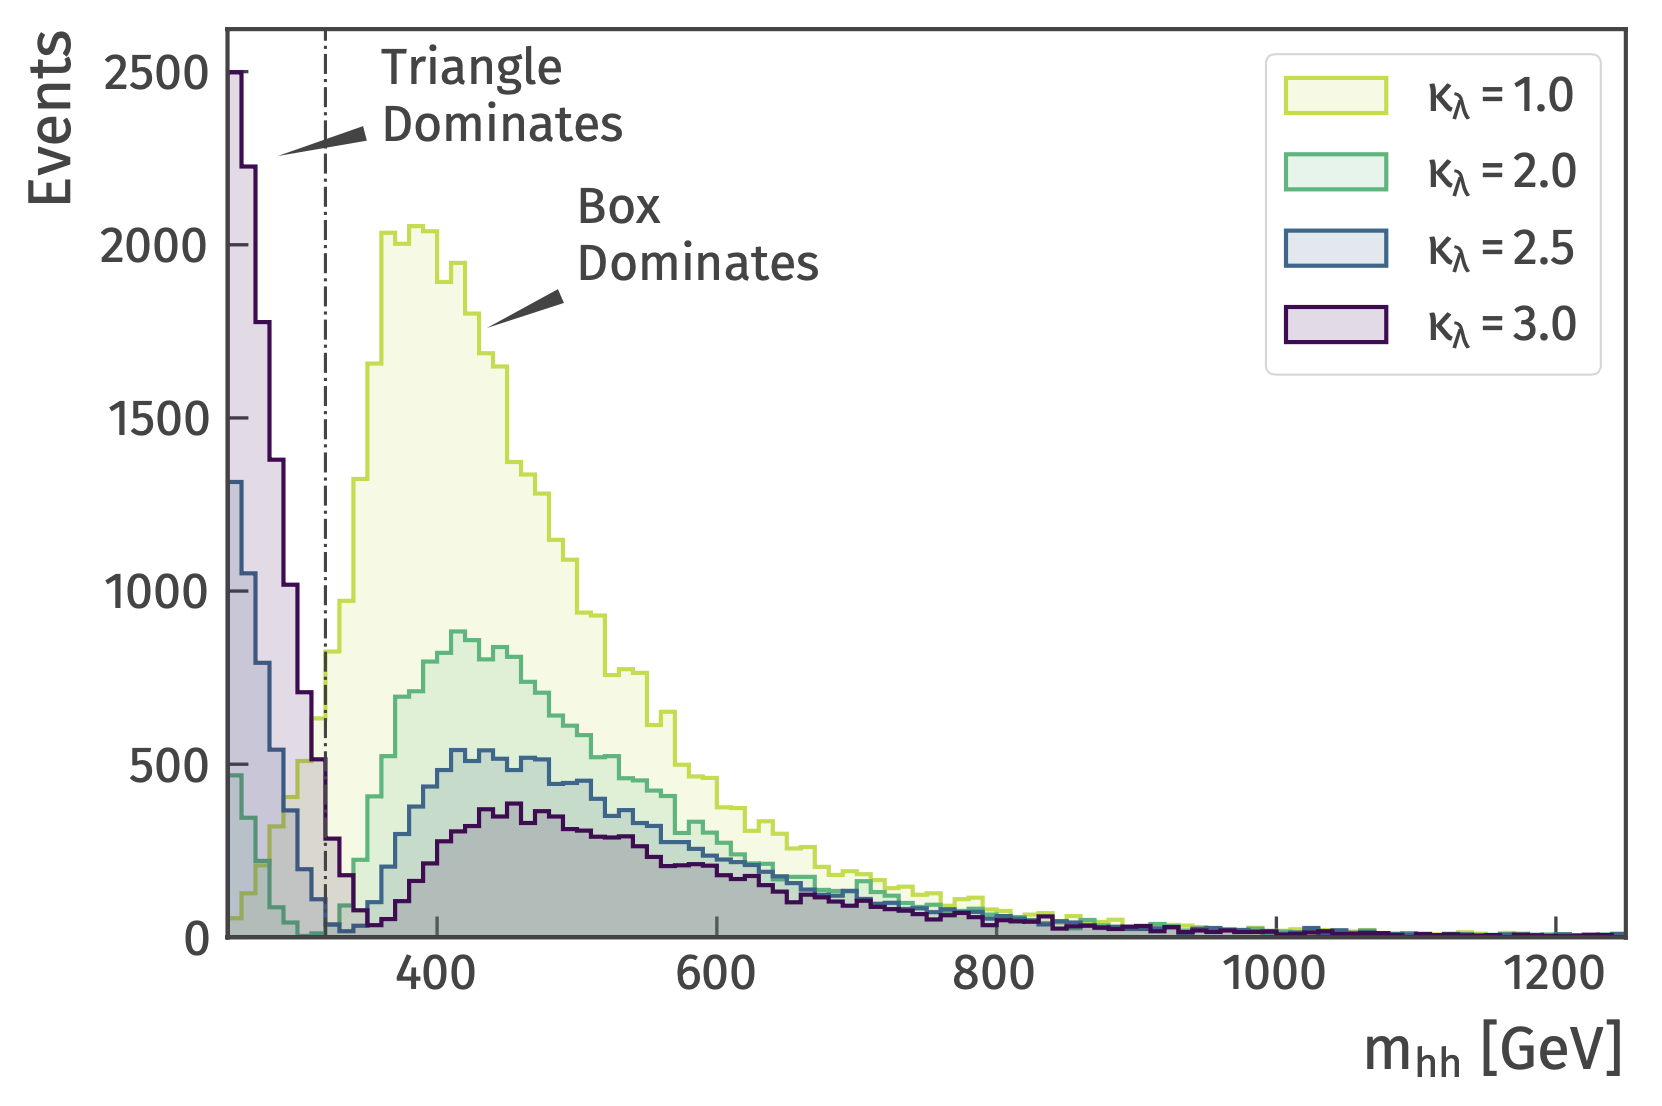
\includegraphics[width=0.49\textwidth]{di-Higgs-SM-kappa-mhh-ref.png}
			\caption{The $m_{hh}$ distribution with various $\kappa_\lambda$. The bin height is weighted by the cross section.}
			\label{fig:di-Higgs-SM-kappa-mhh}
		\end{figure}

		Figure \ref{fig:di-Higgs-SM-kappa-mhh-14TeV} and \ref{fig:di-Higgs-SM-kappa-pth-14TeV} are generated at $\sqrt{s} = 14 \text{ TeV}$. 
		\begin{figure}[htpb]
			\centering
			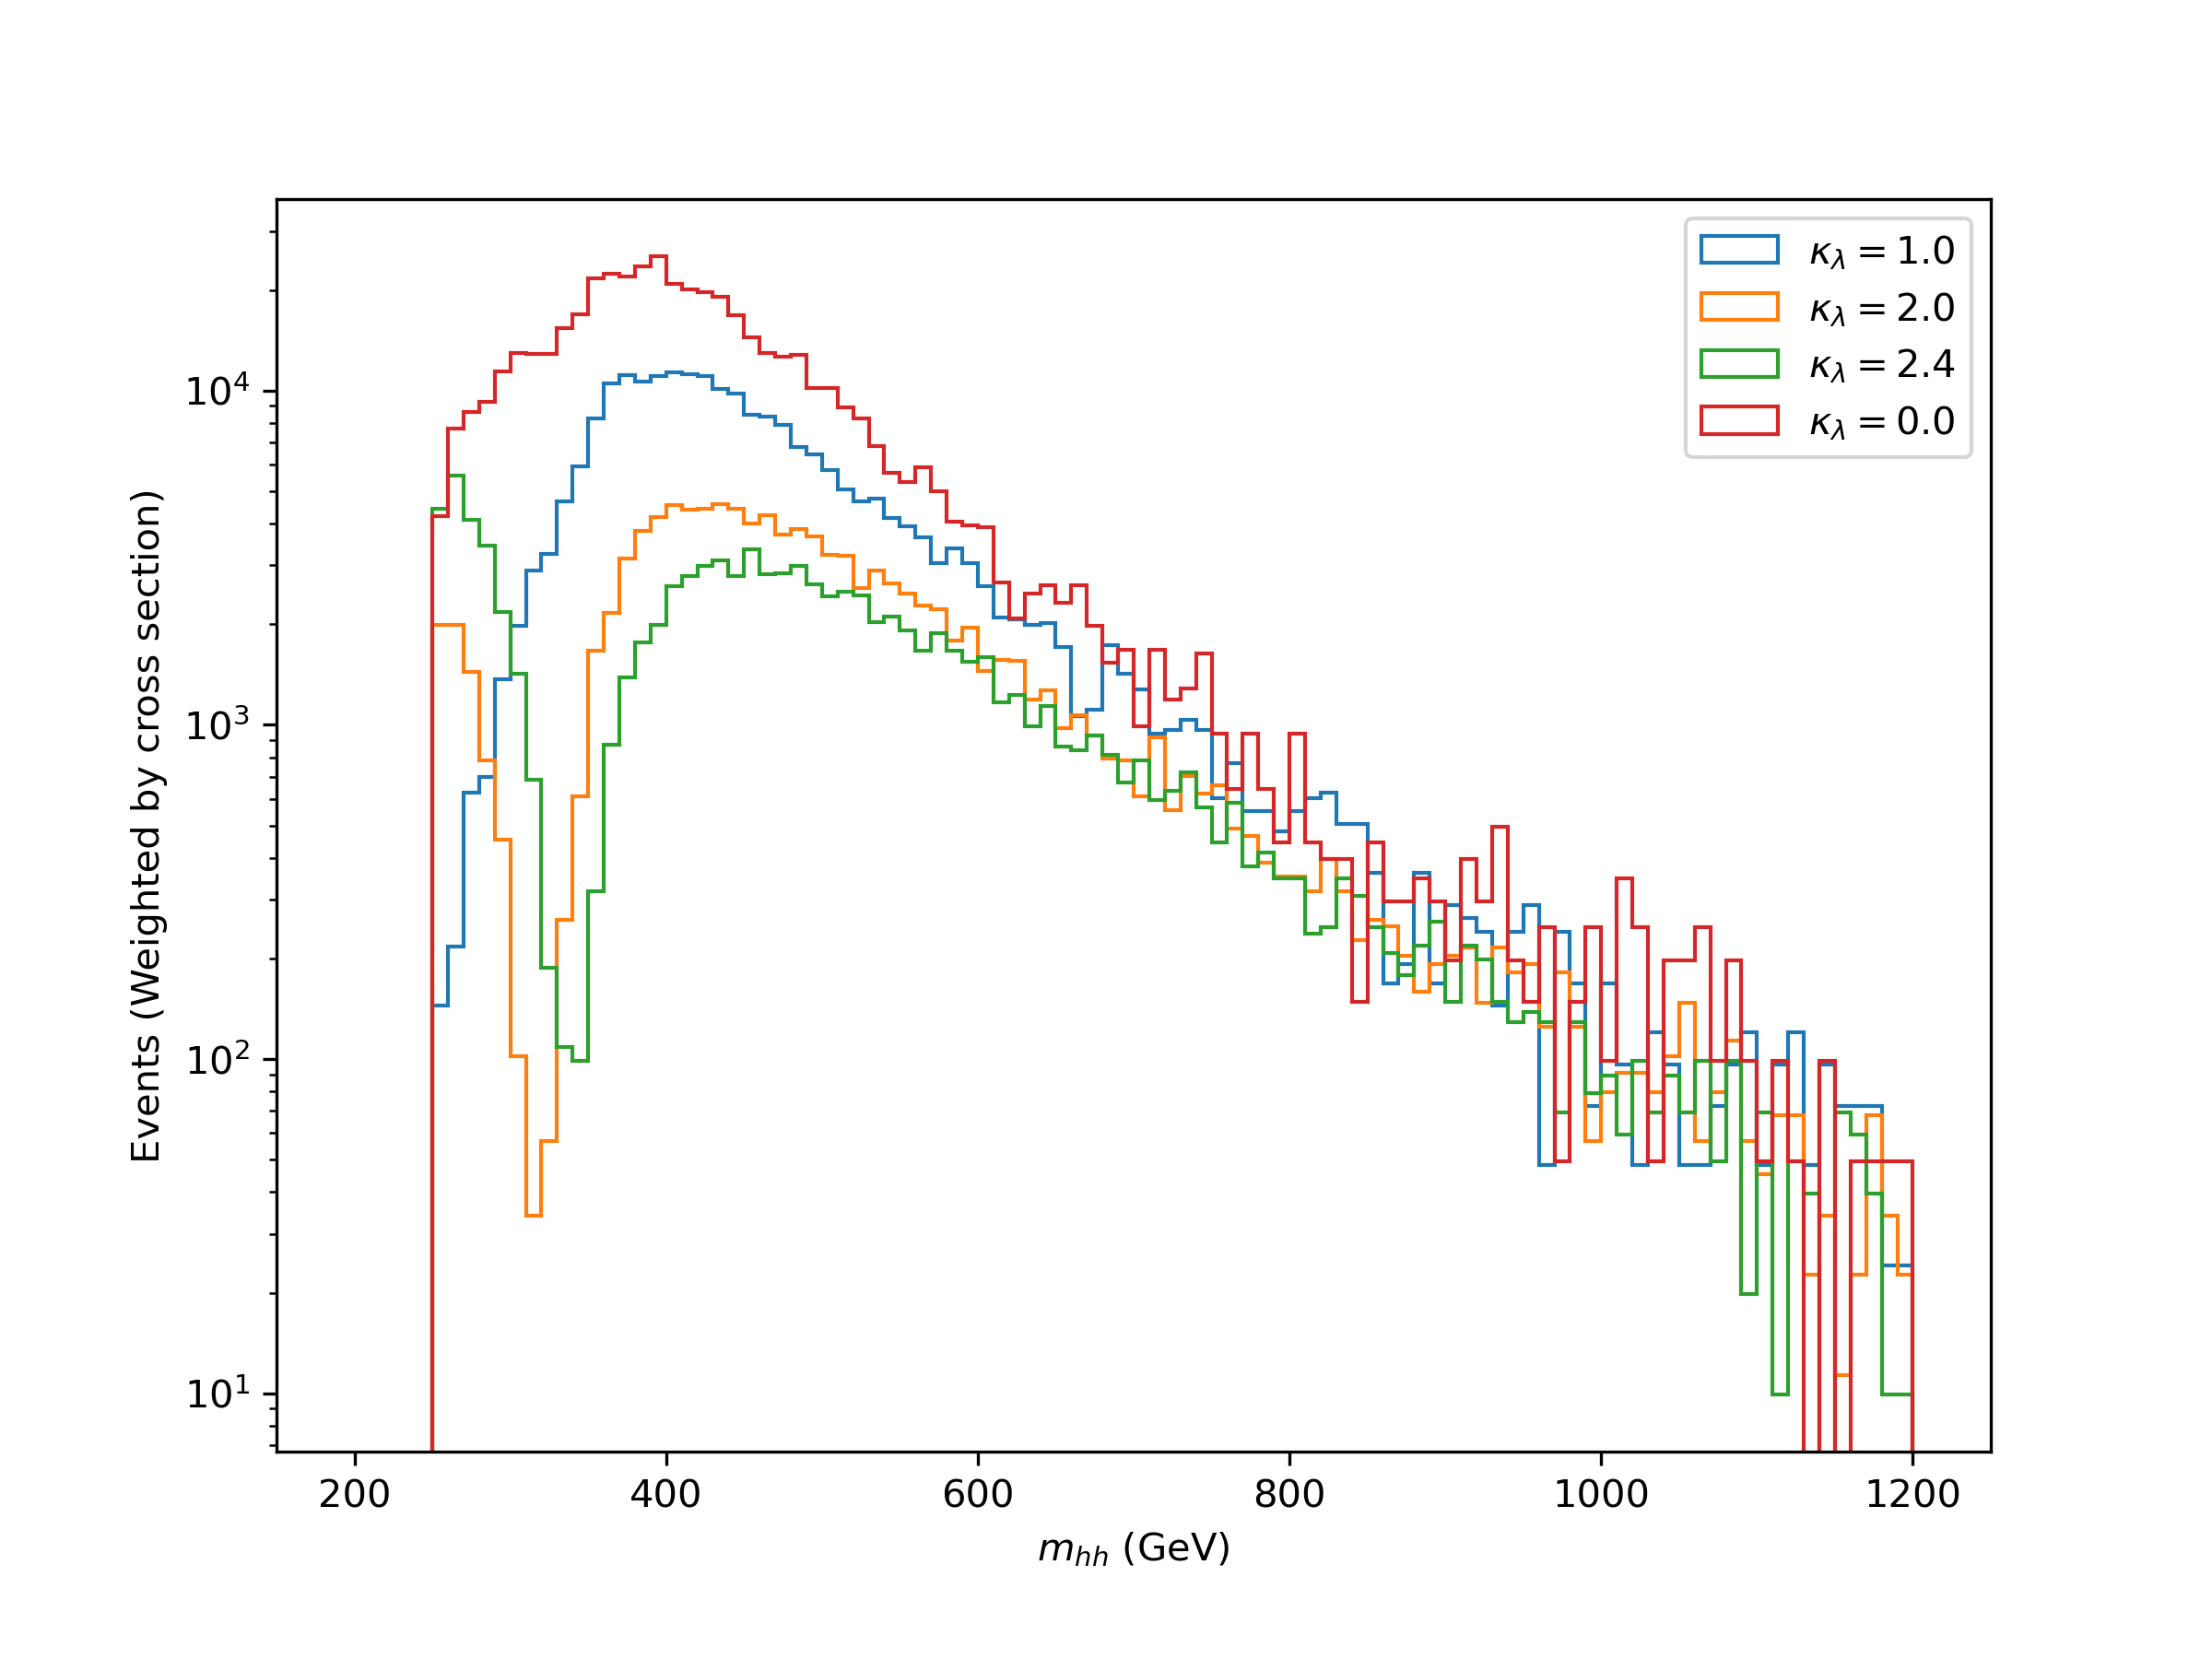
\includegraphics[width=0.49\textwidth]{di-Higgs-SM-kappa-mhh-14TeV-my-data.png}
			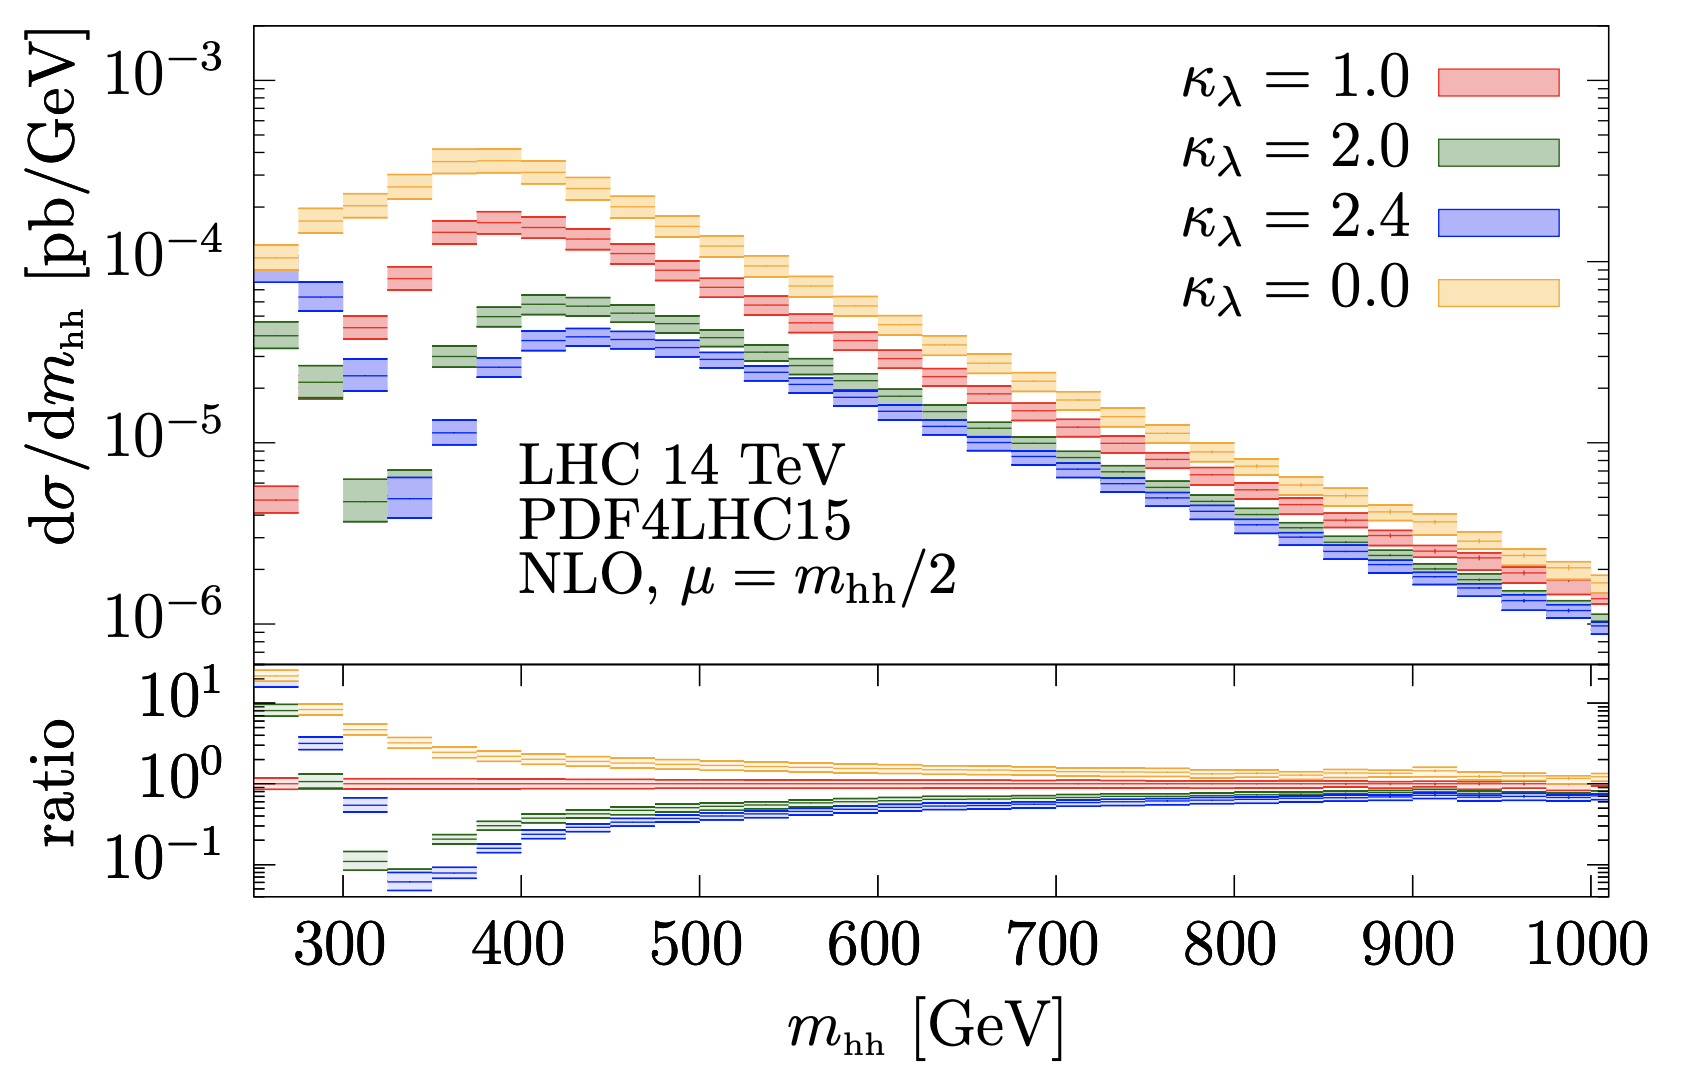
\includegraphics[width=0.49\textwidth]{di-Higgs-SM-kappa-mhh-14TeV-ref.png}
			\caption{The $m_{hh}$ distribution with various $\kappa_\lambda$. The bin height is weighted by the cross section.}
			\label{fig:di-Higgs-SM-kappa-mhh-14TeV}
		\end{figure}
		\begin{figure}[htpb]
			\centering
			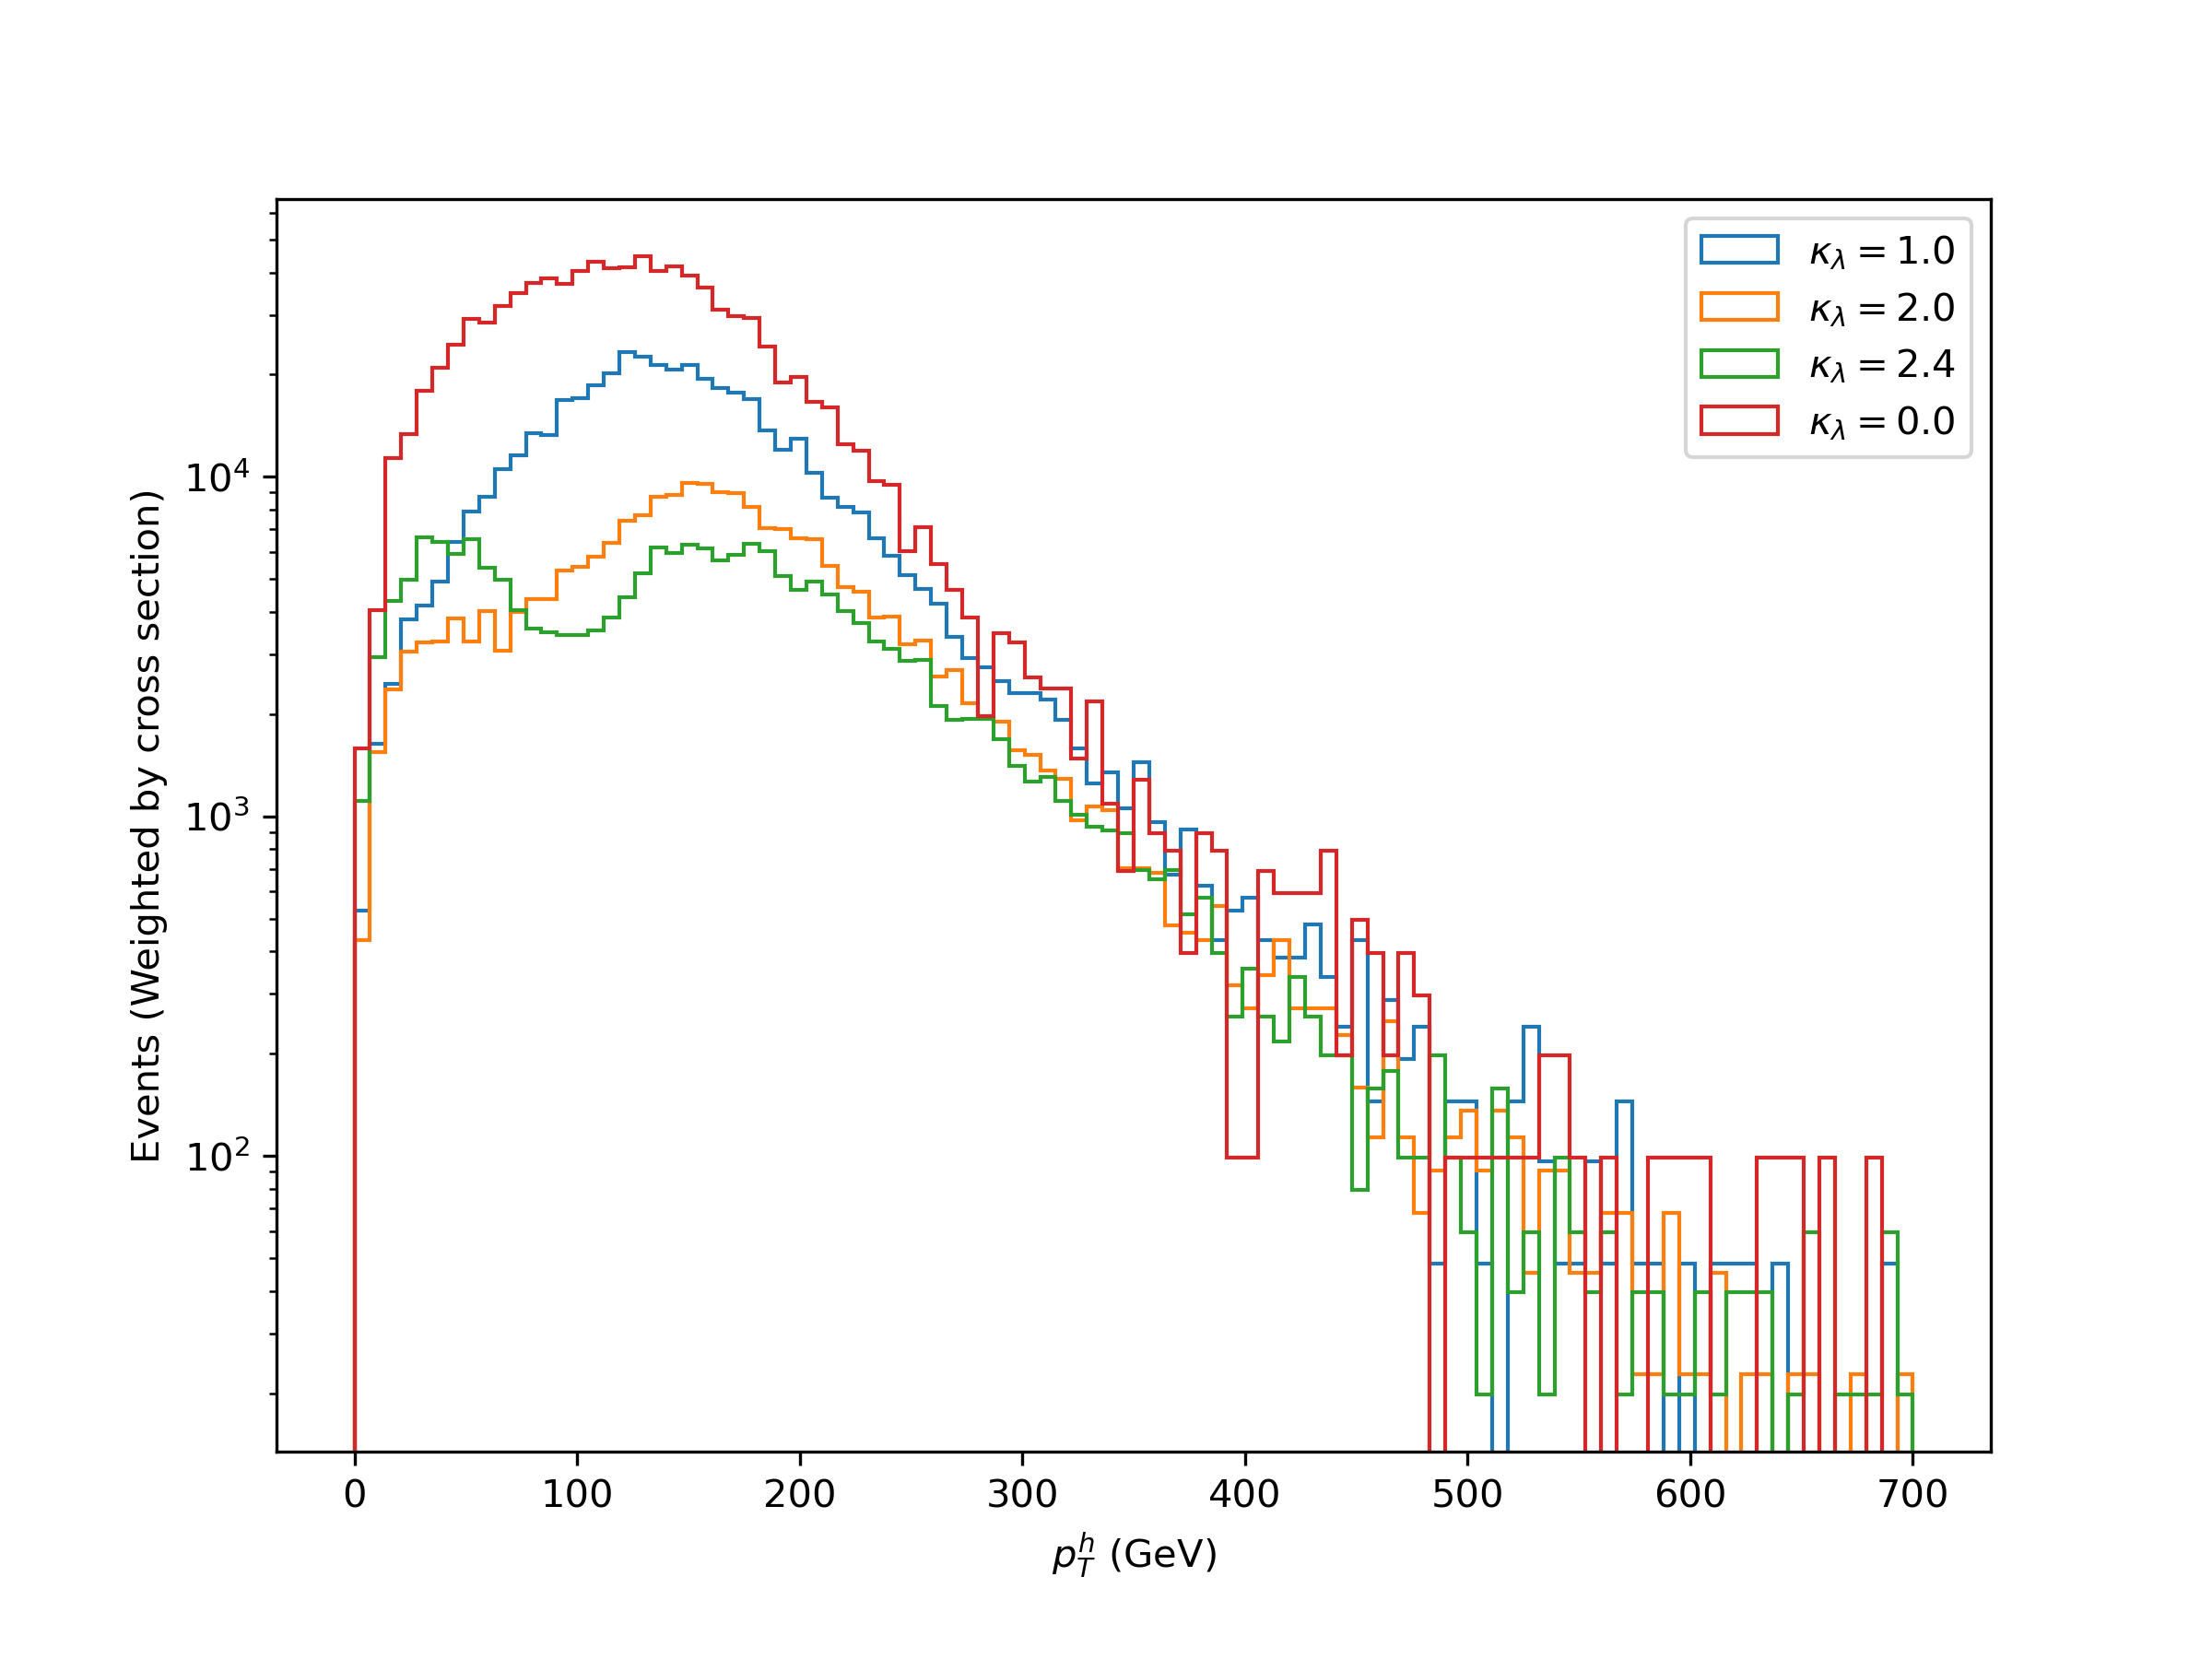
\includegraphics[width=0.49\textwidth]{di-Higgs-SM-kappa-pth-14TeV-my-data.png}
			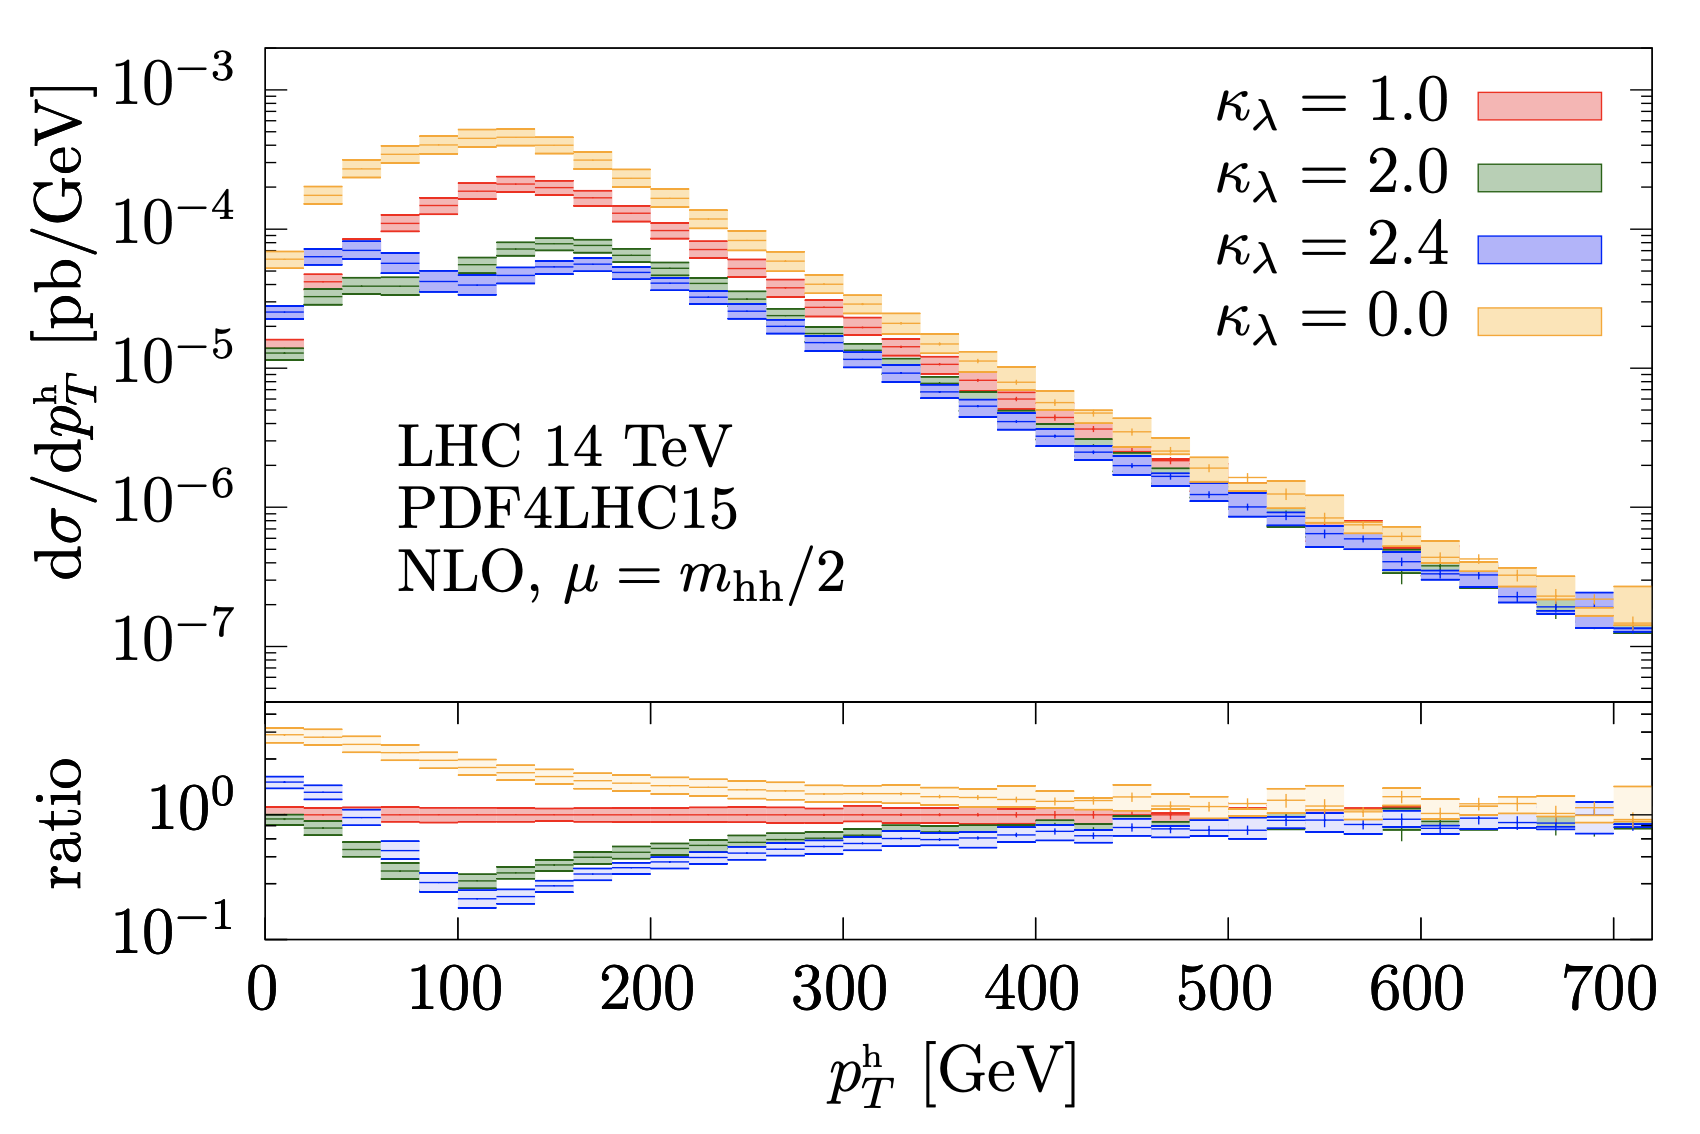
\includegraphics[width=0.49\textwidth]{di-Higgs-SM-kappa-pth-14TeV-ref.png}
			\caption{The $p_\text{T}^{h}$ distribution with various $\kappa_\lambda$. The bin height is weighted by the cross section.}
			\label{fig:di-Higgs-SM-kappa-pth-14TeV}
		\end{figure}

	% subsection di_Higgs_sample_generating_results (end)		
% section generate_di_higgs_samples_in_sm (end)	
\section{Non-resonant di-Higgs event selection}% (fold)
\label{sec:non_resonant_di_higgs_event_selection}
	\subsection{Sample}% (fold)
	\label{sub:sample}
		Non-resonant Higgs pair process is generated by MadGraph. Then pass to Pythia for showering and hadronization. Then pass to Delphes for detector simulation.

		Jets are reconstructed using the anti-$k_t$ algorithm with radius parameter $R = 0.4$.

		The b-tagging part in the Delphes card is changed such that same as the DL1r b-tagger at 77\% WP.  The b-jet efficiency is set to 0.77. The c-jet missing rate is set to 0.204. The light jet missing rate is set to 0.0077.
	% subsection sample (end)

	\subsection{Event selection}% (fold)
	\label{sub:event_selection}
		Reference: \href{https://cds.cern.ch/record/2811390/files/ATLAS-CONF-2022-035.pdf}{ATLAS CONF Note CONF-HDBS-2022-35}

		The selection steps:
		\begin{itemize}
			\item Four tag: The event contains at least 4 b-tagged anti-$k_t$ $R = 0.4$ jets with $p_\text{T} > \text{40 GeV}$ and $\abs{\eta} < 2.5$.
			\item The four jets with the highest $p_\text{T}$ are paired to construct two Higgs boson candidates.
			\item $\text{min-}\Delta R$ pairing method: Choose the pairing in which the higher-$p_\text{T}$ jet pair has the smallest $\Delta R$ separation.
			\item Higgs Eta: 
			\[
				\abs{\Delta\eta_{HH}} < 1.5
			\] 
			\item Top veto: Every possible pair of jets with $p_\text{T} > \text{40 GeV}$ and $\abs{\eta} < 2.5$, including those that were not selected for the $H$ candidates, to form ``$W$ candidates''. ``Top quark candidates'' are built by pairing $W$ candidates with each remaining jet that was selected for $H$ candidates. The quantity $X_{Wt}$ is defined as
			\[
				X_{Wt} = \sqrt{\left( \frac{m_{W} - \text{80.4 GeV}}{0.1 m_{W}} \right)^2 + \left(\frac{m_{t} - \text{172.5 GeV}}{0.1 m_{t}} \right)^2} 
			\] 
			Events with the smallest $X_{Wt} < 1.5$ are vetoed.

			\item Signal region:
			\[
				X_{HH} = \sqrt{\left( \frac{m_{H_1}- \text{124 GeV}}{0.1 m_{H_1}} \right)^2 + \left(\frac{m_{H_2} - \text{117 GeV}}{0.1 m_{H_2}} \right)^2} < 1.6
			\]
			
		\end{itemize}
		\begin{table}[htpb]
			\centering
			\caption{The selection passing rate and efficiency at each stage. The b-tagging part is the same as the DL1r 77\% WP. }
			\label{tab:signal_selection_efficiency_DL1r}
			\begin{tabular}{l|cc|cc}
							  & \multicolumn{2}{|c|}{ATLAS} & \multicolumn{2}{|c}{My sample} \\
				Cut           & pass rate       & efficiency       & pass rate         & efficiency         \\ \hline
				Four tag      & 0.0649 & 0.0649 & 0.0852 & 0.0852 \\
				Higgs Eta     & 0.0543 & 0.8360 & 0.0688 & 0.8074 \\
				Top veto      & 0.0456 & 0.8401 & 0.0553 & 0.8044 \\
				Signal region & 0.0220 & 0.4818 & 0.0181 & 0.3283 \\
			\end{tabular}
		\end{table}

		Correct selection:
		Consider the events in which four jets can be matched one-to-one (within $\Delta R < 0.3$) to the four b-quarks decayed from the Higgs bosons. For the highest $p_\text{T} $ there are 89\% of simulated signal events reaching this selection.	

		Correct pairing: Consider the correct selection events, for $\text{min-}\Delta R$ pairing method there 85\% of events are correctly paired.

		Figure \ref{fig:Higgs_mass_new} shows the Higgs mass distribution. There is a deviation between the mass distribution peak and the signal region's center.  
		\begin{figure}[htpb]
			\centering
			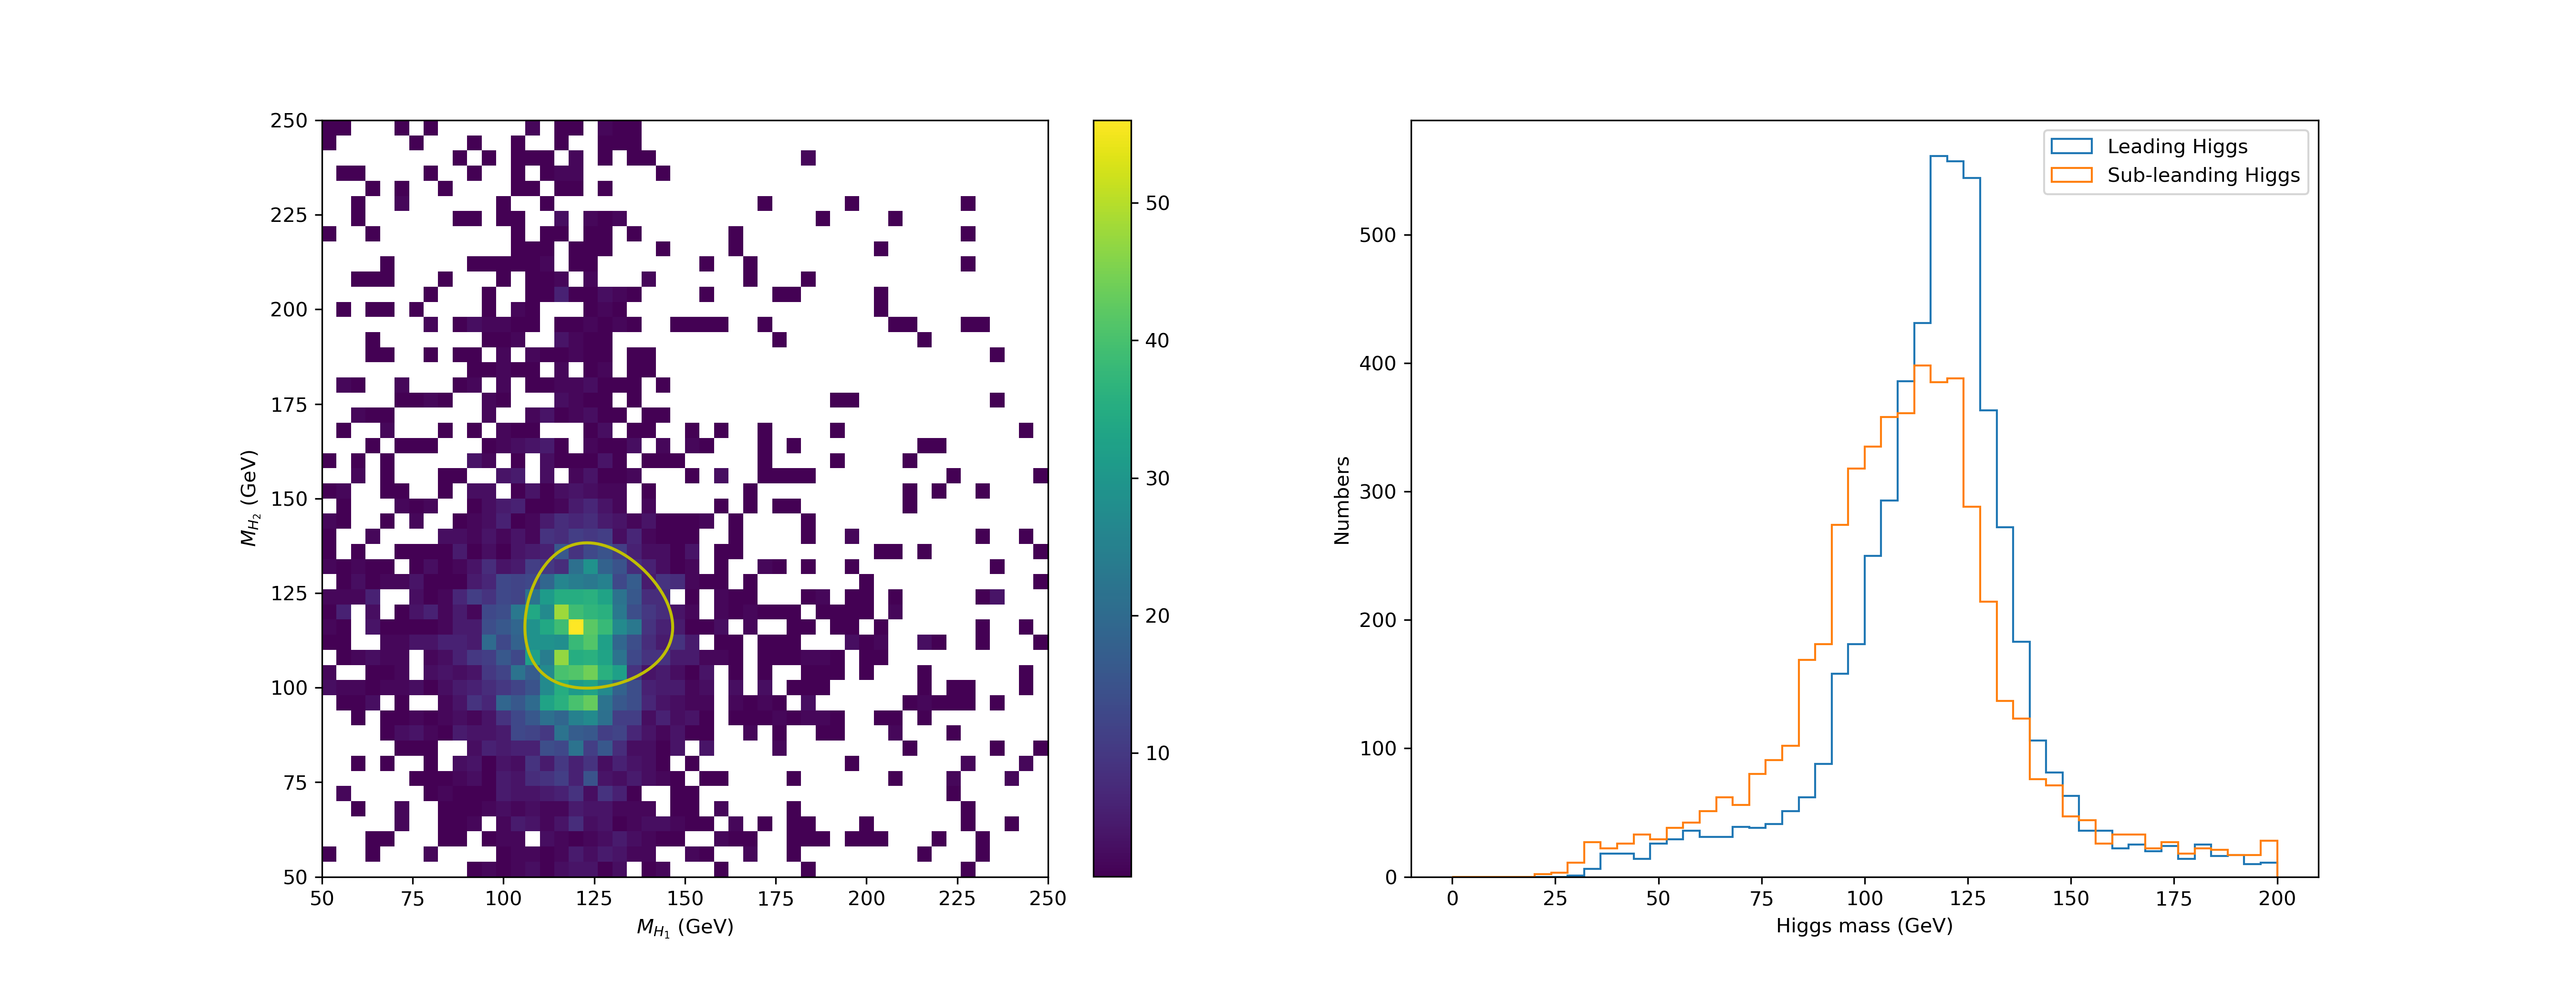
\includegraphics[width=0.97\textwidth]{Higgs_mass_new_s.png}
			\caption{The mass plane and distribution for Higgs candidate.}
			\label{fig:Higgs_mass_new}
		\end{figure}

		\subsubsection{Old method}% (fold)
		\label{subs:subsubsection_name}
			Reference: \href{https://arxiv.org/pdf/1804.06174.pdf}{Search for pair production of Higgs bosons in the $b\overline{b}b\overline{b}$ final state using proton-proton collisions at $\sqrt{s} = \text{13 TeV}$ with the ATLAS detector}

			The selection steps:
			\begin{itemize}
			\item Four tag: The event contains at least 4 b-tagged anti-kt small-$R$ ($R = 0.4$) jets with $p_\text{T} > \text{40 GeV}$ and $\abs{\eta} < 2.5$. The four jets with the highest b-tagging score are paired to construct two Higgs boson candidates.
			\item The four jets with the highest $p_\text{T}$ are paired to construct two Higgs boson candidates in my samples.
			\item Delta R: Pairing jets to Higgs boson candidate need to satisfy the following requirements:
			\[
				\left.
				\begin{array}{c}
					\dfrac{\text{360 GeV}}{m_\text{4j}} - 0.5 < \Delta R_{jj,\text{lead}} < \dfrac{\text{653 GeV}}{m_{\text{4j}}} + 0.475 \\
					\dfrac{\text{235 GeV}}{m_\text{4j}}  < \Delta R_{jj,\text{subl}} < \dfrac{\text{875 GeV}}{m_{\text{4j}}} + 0.35 
				\end{array} 
				\right\} \text{ if } m_{\text{4j}} <  \text{1250 GeV}
			\] 
			\[
				\left.
				\begin{array}{c}
					0 < \Delta R_{jj,\text{lead}} < 1 \\
					0 < \Delta R_{jj,\text{subl}} < 1 
				\end{array} 
				\right\} \text{ if } m_{\text{4j}} >  \text{1250 GeV}
			\] 
			\item If there are more than 2 pairings satisfies the Delta R requirement. Calculate $D_{HH}$
			\[
				D_{HH} = \frac{\abs{m_{\text{2j}}^{\text{lead}} - \frac{120}{110} m_{\text{2j}}^{\text{subl}}}}{\sqrt{1 + \left( \frac{120}{110} \right)^2}}
			\] 
			the pairing with the smallest value of $D_{HH}$ is chosen.
			\item Higgs PT: 
			\begin{align*}
				p_{\text{T}}^{\text{lead}} &> m_{\text{4j}} \times 0.5 - \text{103 GeV} \\
				p_{\text{T}}^{\text{subl}} &> m_{\text{4j}} \times 0.33 - \text{73 GeV} \\
			\end{align*}
			\item Higgs Eta: 
			\[
				\abs{\Delta\eta_{HH}} < 1.5
			\] 
			\item Signal region:
			\[
				X_{HH} = \sqrt{\left( \frac{m_{\text{2j}}^{\text{lead}} - \text{120 GeV}}{0.1 m_{\text{2j}}^{\text{lead}}} \right)^2 + \left(\frac{m_{\text{2j}}^{\text{subl}} - \text{110 GeV}}{0.1 m_{\text{2j}}^{\text{subl}}} \right)^2} < 1.6
			\]
			\item Top veto: Every possible pair of jets with $p_\text{T} > \text{40 GeV}$ and $\abs{\eta} < 2.5$, including those that were not selected for the $H$ candidates, to form ``$W$ candidates''. ``Top quark candidates'' are built by pairing $W$ candidates with each remaining jet that was selected for $H$ candidates
			\[
				X_{Wt} = \sqrt{\left( \frac{m_{W} - \text{80 GeV}}{0.1 m_{W}} \right)^2 + \left(\frac{m_{t} - \text{173 GeV}}{0.1 m_{t}} \right)^2} 
			\] 
			Events with the smallest $X_{Wt} < 1.5$ are vetoed.

			\end{itemize}

			The results are in Table \ref{tab:signal_selection_efficiency_MV2c10}.
			\begin{table}[htpb]
				\centering
				\caption{The selection passing rate and efficiency at each stage.}
				\label{tab:signal_selection_efficiency_MV2c10}

				\begin{tabular}{l|cc|cc}
								  & \multicolumn{2}{|c|}{ATLAS} & \multicolumn{2}{|c}{My sample} \\
					Cut           & pass rate       & efficiency       & pass rate         & efficiency         \\ \hline
					Four tag      & 0.0490 & 0.0490 & 0.0563 & 0.0563 \\
					Delta R       & 0.0448 & 0.9143 & 0.0471 & 0.8370 \\
					Higgs PT      & 0.0422 & 0.9420 & 0.0446 & 0.9480 \\
					Higgs Eta     & 0.0380 & 0.9005 & 0.0398 & 0.8911 \\
					Signal region & 0.0193 & 0.5079 & 0.0170 & 0.4280 \\
					Top veto      & 0.0179 & 0.9275 & 0.0145 & 0.8537
				\end{tabular}
			\end{table}
			
		% subsubsection subsubsection_name (end)	

	% subsection event_selection (end)	
	\subsection{Background event selection}% (fold)
	\label{sub:background_event_selection}
		Apply the same selection step to the background samples. The cutflow table is in Table \ref{tab:signal_selection_efficiency_pp4b} and the mass distribution is in Figure \ref{fig:Higgs_mass_new_pp4b}.
		\begin{table}[htpb]
			\centering
			\caption{The selection passing rate and efficiency at each stage for ``$\text{min-}\Delta R$'' pairing method.}
			\label{tab:signal_selection_efficiency_pp4b}
			\begin{tabular}{l|cc}
							  & \multicolumn{2}{c}{pp4b}                                                         \\
							  & \multicolumn{2}{c}{$\text{min-}\Delta R$}\\
				Cut           & pass rate               & efficiency                \\ \hline
				Four tag      & 0.0096                  & 0.0096                    \\
				Higgs Eta     & 0.0056                  & 0.5835                    \\
				Top veto      & 0.0042                  & 0.7423                    \\
				Signal region & 0.0001                  & 0.0232                    \\
			\end{tabular}
		\end{table}
		\begin{figure}[htpb]
			\centering
			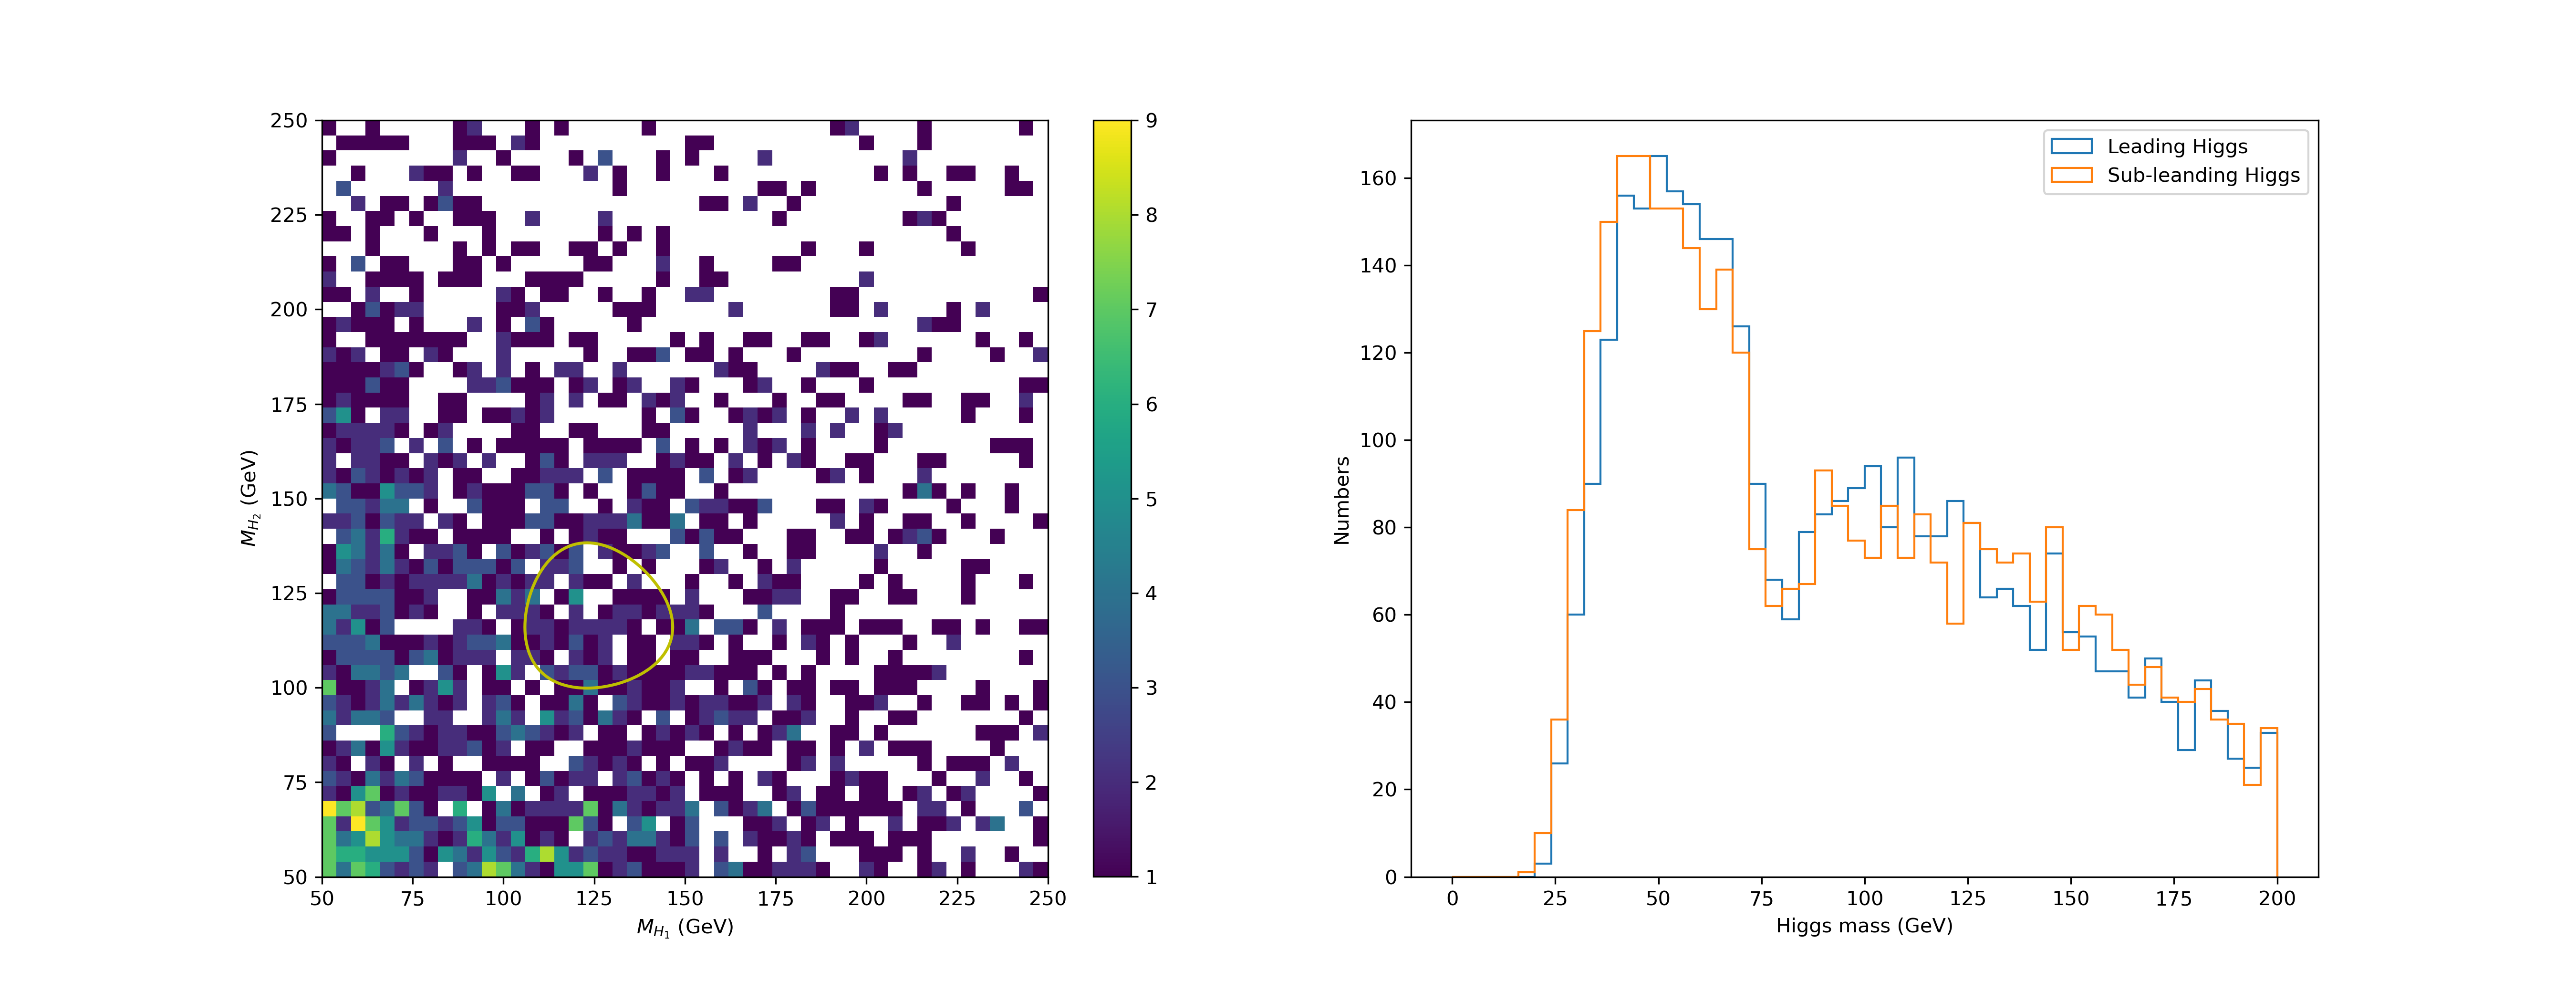
\includegraphics[width=0.97\textwidth]{Higgs_mass_new_mindR_pp4b.png}
			\caption{The mass plane and distribution for background events Higgs candidate.}
			\label{fig:Higgs_mass_new_pp4b}
		\end{figure}

	% subsection background_event_selection (end)		
	
% section non_resonant_di_higgs_event_selection (end)		
\section{Apply SPANET on non-resonant di-Higgs event}% (fold)
\label{sec:apply_spanet_on_non_resonant_di_higgs_event}
	\subsection{Training SPANET}% (fold)
	\label{sub:training_spanet}
		The training samples are required to pass the ``Four tag cut'', i.e., there are at least four b-tagged jets with $p_{\text{T}} > \text{40 GeV}$ and $\abs{\eta} < 2.5$. The b-tagging efficiency is the same as the DL1r b-tagger at 77\% WP.
		\begin{itemize}
			\item Training sample:
			\begin{itemize}
				\item Total sample size: 76,131
				\item 1h sample size: 14,527
				\item 2h sample size: 60,122			
				\item 5\% used on validation
			\end{itemize}
			\item Testing sample: 
			\begin{itemize}
				\item Total sample size: 8,460
				\item 1h sample size: 1,577
				\item 2h sample size: 6,744
			\end{itemize}
		\end{itemize}
		The training results are presented in Table \ref{tab:SPANet_diHiggs_4btag_DL1r_pt40}.
		\begin{table}[htpb]
			\centering
			\caption{SPA-NET training results on the di-Higgs samples with ``Four tag cut''.}
			\label{tab:SPANet_diHiggs_4btag_DL1r_pt40}
			\begin{tabular}{c|c|cc}
				$N_\text{Jet}$ & Event Fraction & Event Efficiency & Higgs Efficiency \\
				\hline
				$=4$	  &   0.280             &    0.961              &    0.961             \\
				$=5$	  &   0.287             &    0.878              &    0.913             \\
				$\ge 6$	  &   0.229             &    0.740              &    0.819             \\
				Total	  &   0.797             &    0.868              &    0.903             \\
			\end{tabular}
		\end{table}

	% subsection training_spanet (end)
	\subsection{Use SPANET for event selection}% (fold)
	\label{sub:use_spanet_for_event_selection}
		The ``$ \text{min-}\Delta R$'' pairing is replaced by SPA-NET pairing. Other cuts remained unchanged. The cutflow tables for signal and background are in Table \ref{tab:signal_selection_efficiency_SPANet}, \ref{tab:signal_selection_efficiency_background_SPANet}.
		\begin{table}[htpb]
			\centering
			\caption{The selection passing rate and efficiency at each stage for ``$\text{min-}\Delta R$'' and SPA-NET pairing.}
			\label{tab:signal_selection_efficiency_SPANet}
			\begin{tabular}{l|cc|cc|cc}
					& \multicolumn{4}{c|}{$\text{min-}\Delta R$}                               & \multicolumn{2}{c}{SPA-NET}   \\
							  & \multicolumn{2}{c|}{ATLAS} & \multicolumn{2}{c|}{My sample}             & \multicolumn{2}{c}{My sample} \\
				Cut           & pass rate   & efficiency  & pass rate & \multicolumn{1}{c|}{efficiency} & pass rate     & efficiency    \\ \hline
				Four tag      & 0.0649 & 0.0649 & 0.0852 & 0.0852 & 0.0852 & 0.0852\\
				Higgs Eta     & 0.0543 & 0.8360 & 0.0688 & 0.8074 & 0.0635 & 0.7454\\
				Top veto      & 0.0456 & 0.8401 & 0.0553 & 0.8044 & 0.0508 & 0.8006\\
				Signal region & 0.0220 & 0.4818 & 0.0181 & 0.3283 & 0.0027 & 0.0541\\
			\end{tabular}
		\end{table}
		\begin{table}[htpb]
			\centering
			\caption{The selection passing rate and efficiency at each stage for ``$\text{min-}\Delta R$'' and SPA-NET pairing. }
			\label{tab:signal_selection_efficiency_background_SPANet}
			\begin{tabular}{l|cc|cc}
							  & \multicolumn{4}{c}{pp4b}                                                         \\
							  & \multicolumn{2}{c|}{$\text{min-}\Delta R$}& \multicolumn{2}{c}{SPA-NET} \\
				Cut           & pass rate               & efficiency                & pass rate    & efficiency   \\ \hline
				Four tag      & 0.0096                  & 0.0096                    & 0.0096       & 0.0096       \\
				Higgs Eta     & 0.0056                  & 0.5835                    & 0.0055       & 0.5733       \\
				Top veto      & 0.0042                  & 0.7423                    & 0.0042       & 0.7607      \\
				Signal region & 0.0001                  & 0.0232                    & 0.0001       & 0.0181       \\
			\end{tabular}
		\end{table}

		Figure \ref{fig:Higgs_mass_new_SPANET_wrong} shows the Higgs mass distribution for SPA-NET pairing.
		\begin{figure}[htpb]
			\centering
			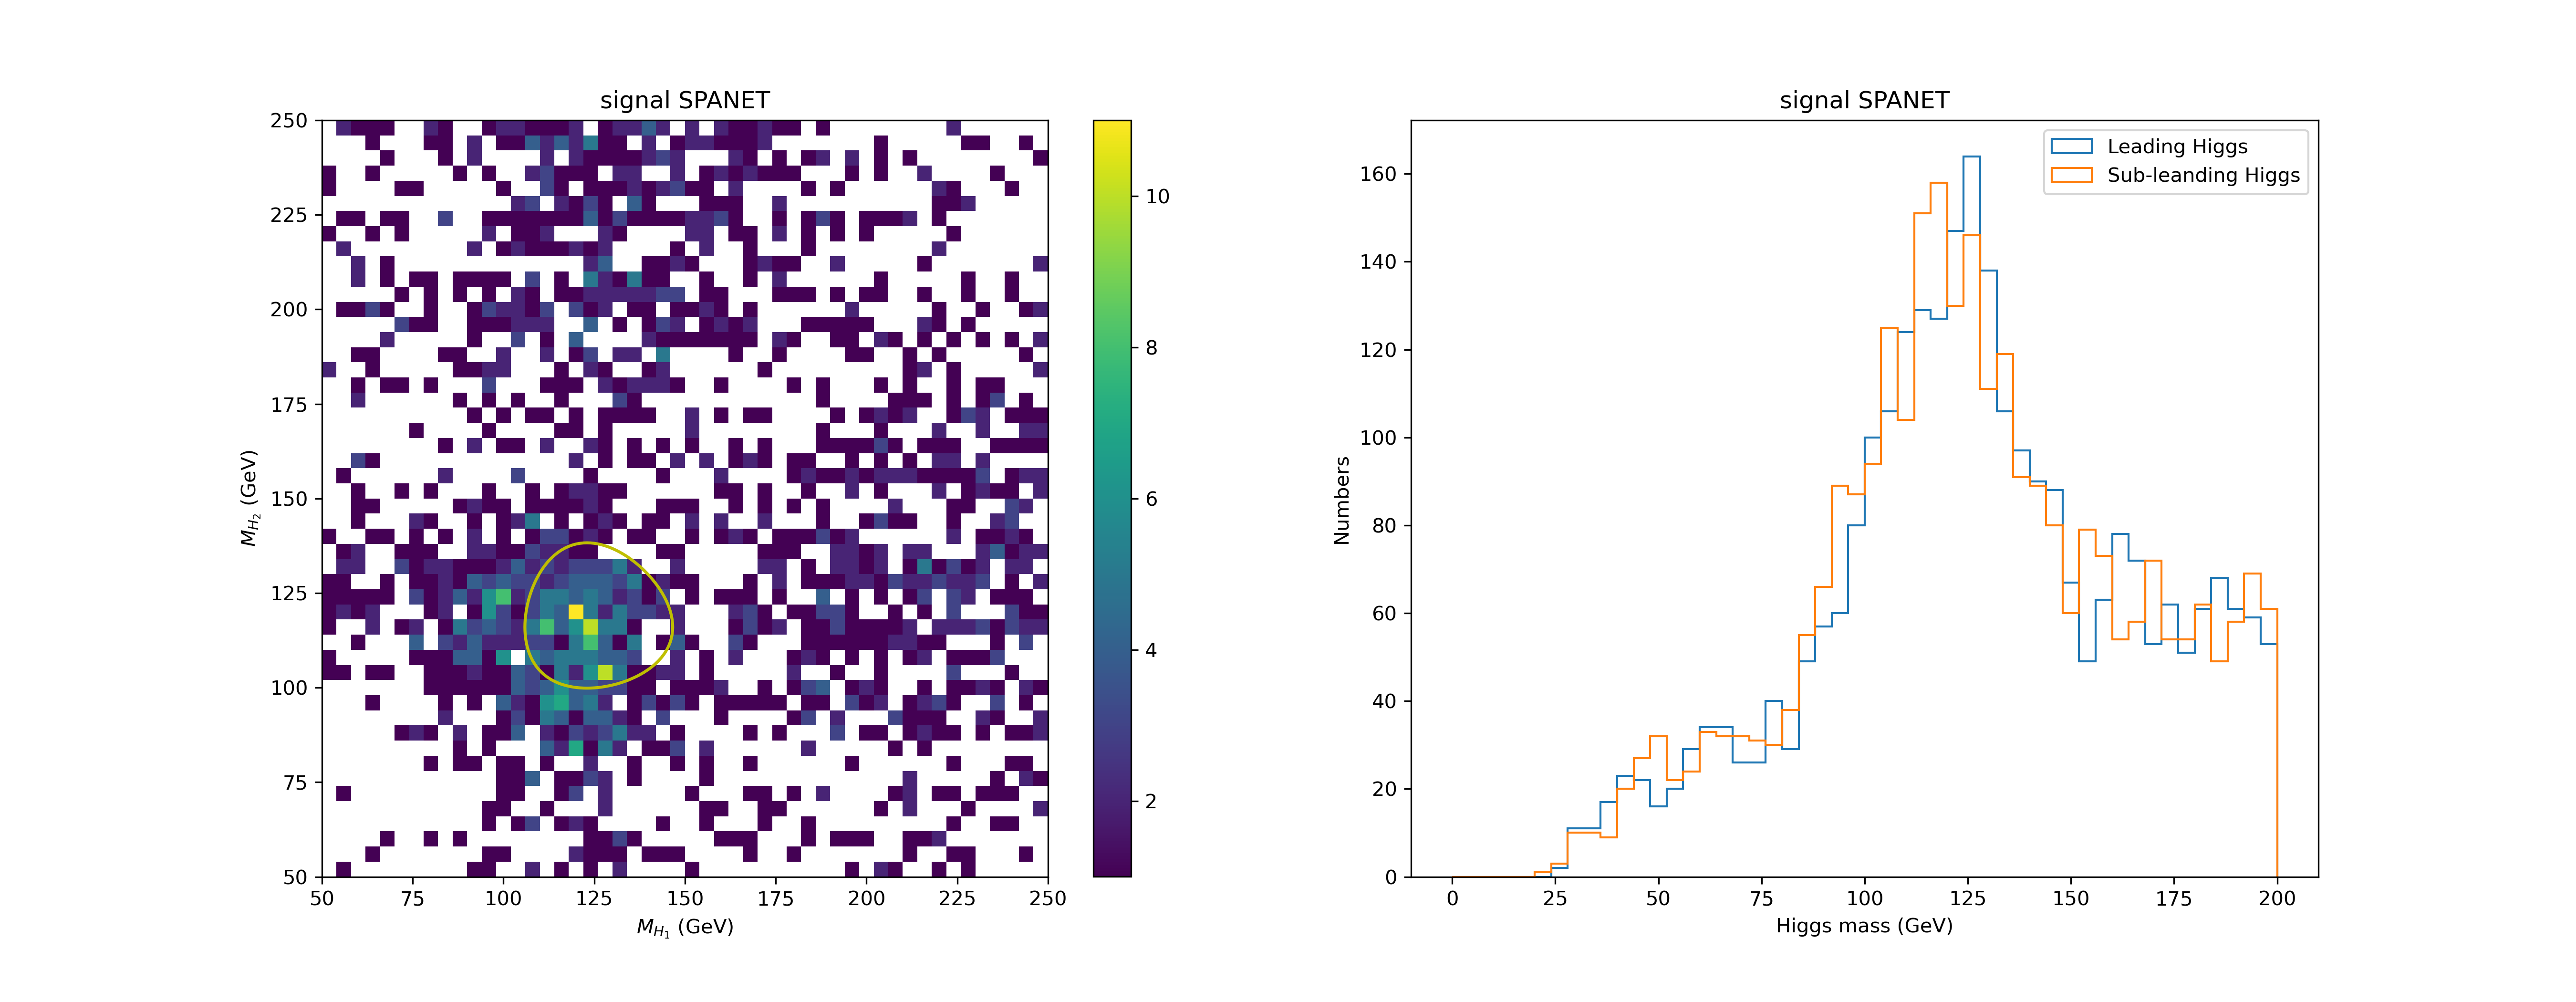
\includegraphics[width=0.97\textwidth]{Higgs_mass_new_SPANET_wrong_s.png}
			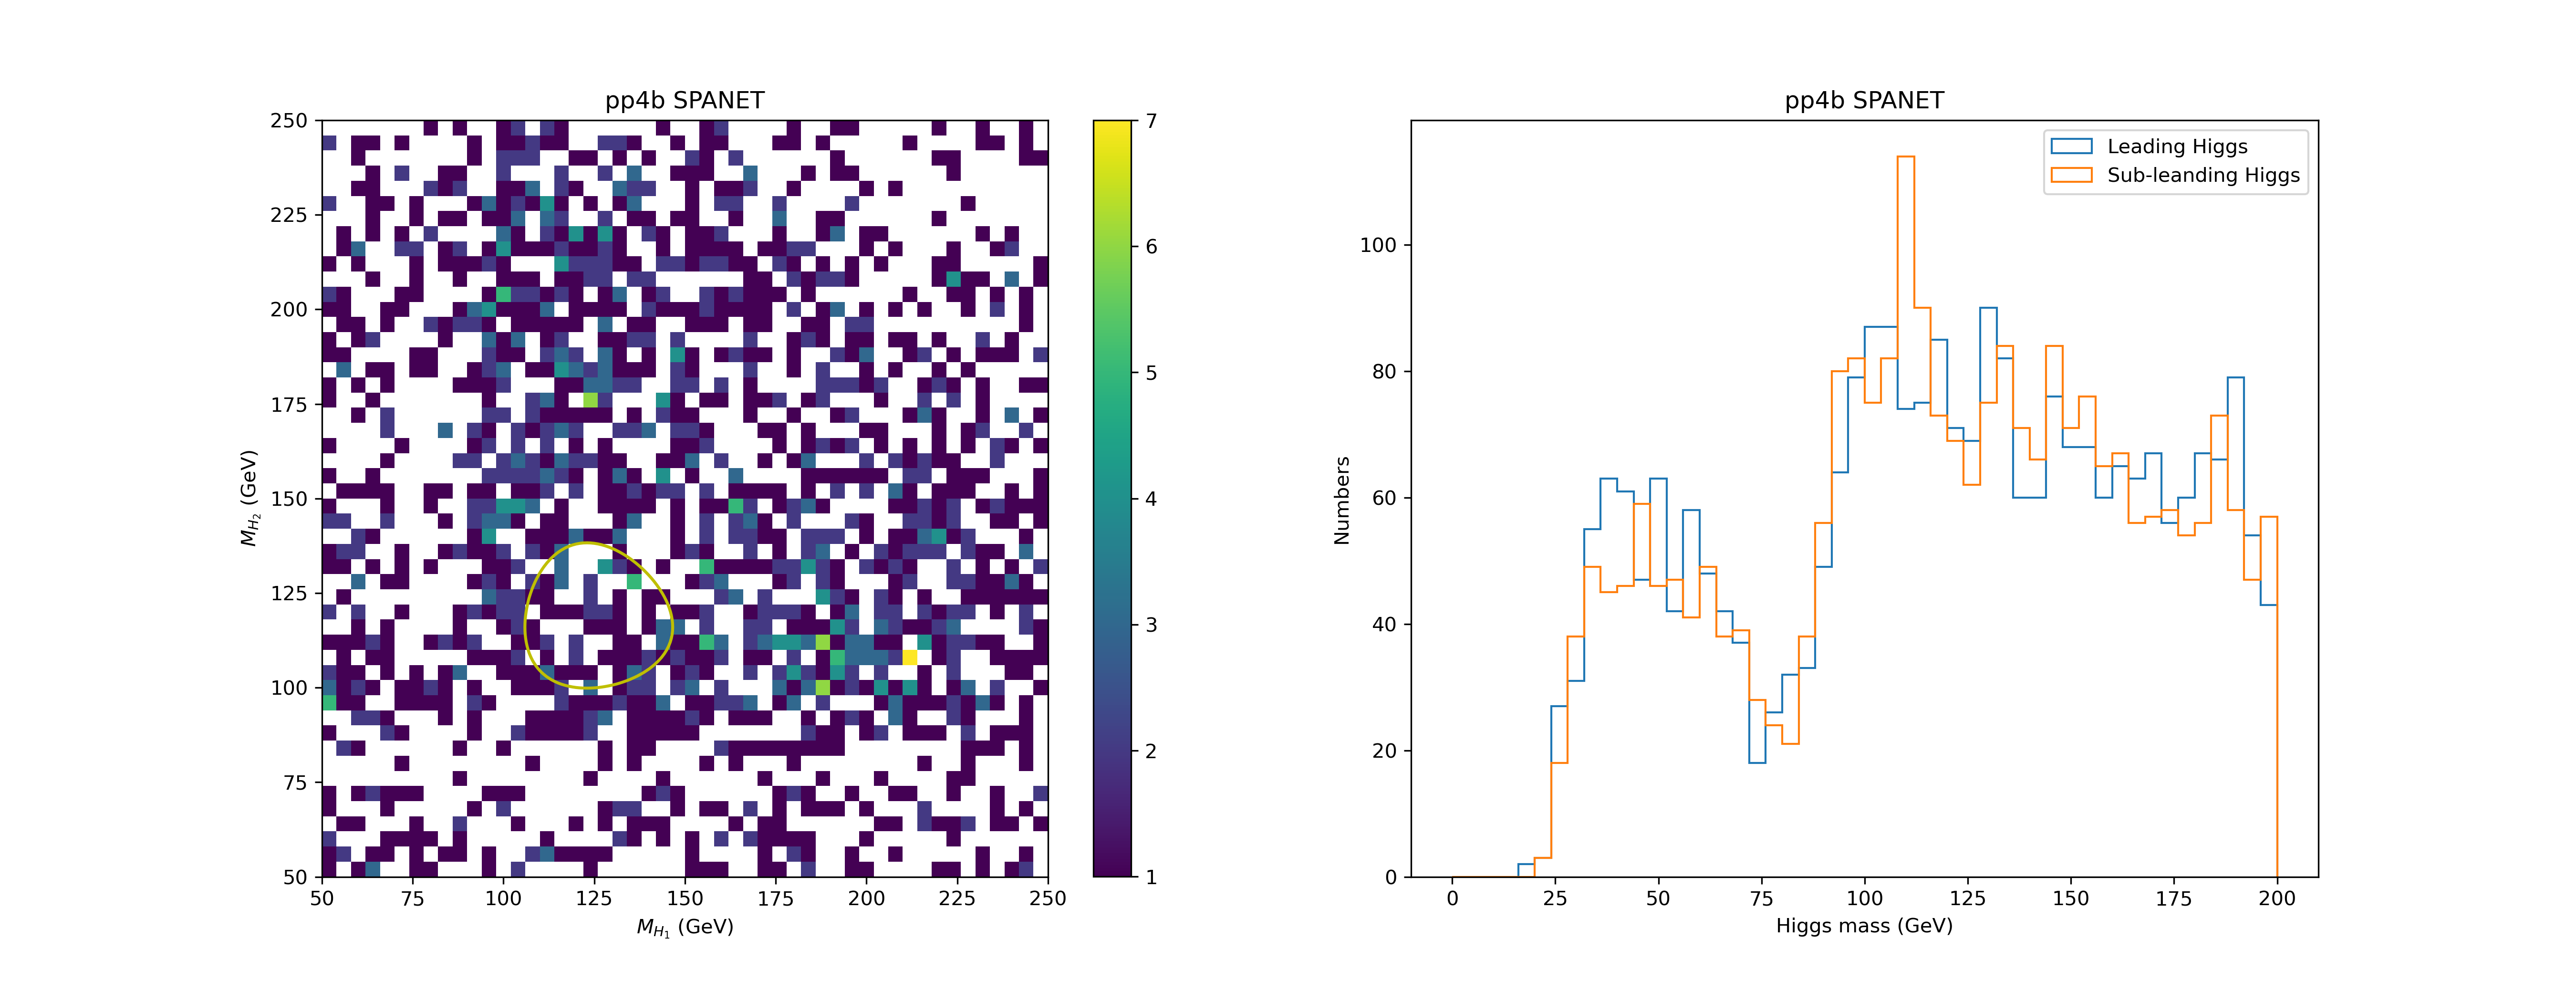
\includegraphics[width=0.97\textwidth]{Higgs_mass_new_SPANET_wrong_4b.png}
			\caption{The mass plane and distribution for Higgs candidate for SPA-NET pairing method. The above figure is for the signal sample and the below one is for the background sample.}
			\label{fig:Higgs_mass_new_SPANET_wrong}
		\end{figure}


	% subsection use_spanet_for_event_selection (end)	
% section apply_spanet_on_non_resonant_di_higgs_event (end)			
\section{Pairing performace}% (fold)
\label{sec:pairing_performace}

	The truth pairing is defined by matching the jets to the simulated quarks within the angular distance of $\Delta R = \sqrt{(\Delta\eta)^2 + (\Delta\phi)^2} < 0.4$.
	
	The ``$\text{min-}\Delta R$ '' pairing method contain two-step: first select four b-jets with the highest $p_\text{T}$, and second, choose $\text{min-}\Delta R$ configuration. For the first step, the correct selection rate is $89\%$. For the second step, the correct pairing rate is  $91 \%$. The pairing efficiency is  $81 \%$.

	The ``SPA-NET'' pairing method:  The pairing efficiency is  $86.8 \%$.

	The mass distribution for truth pairing is in Figure \ref{fig:Higgs_mass_new_truth}. The results are similar to the ``$\text{min-}\Delta R$'' ones, but much different to the SPA-NET's. There are indeed some bugs in the SPA-NET pairing code.
		\begin{figure}[htpb]
			\centering
			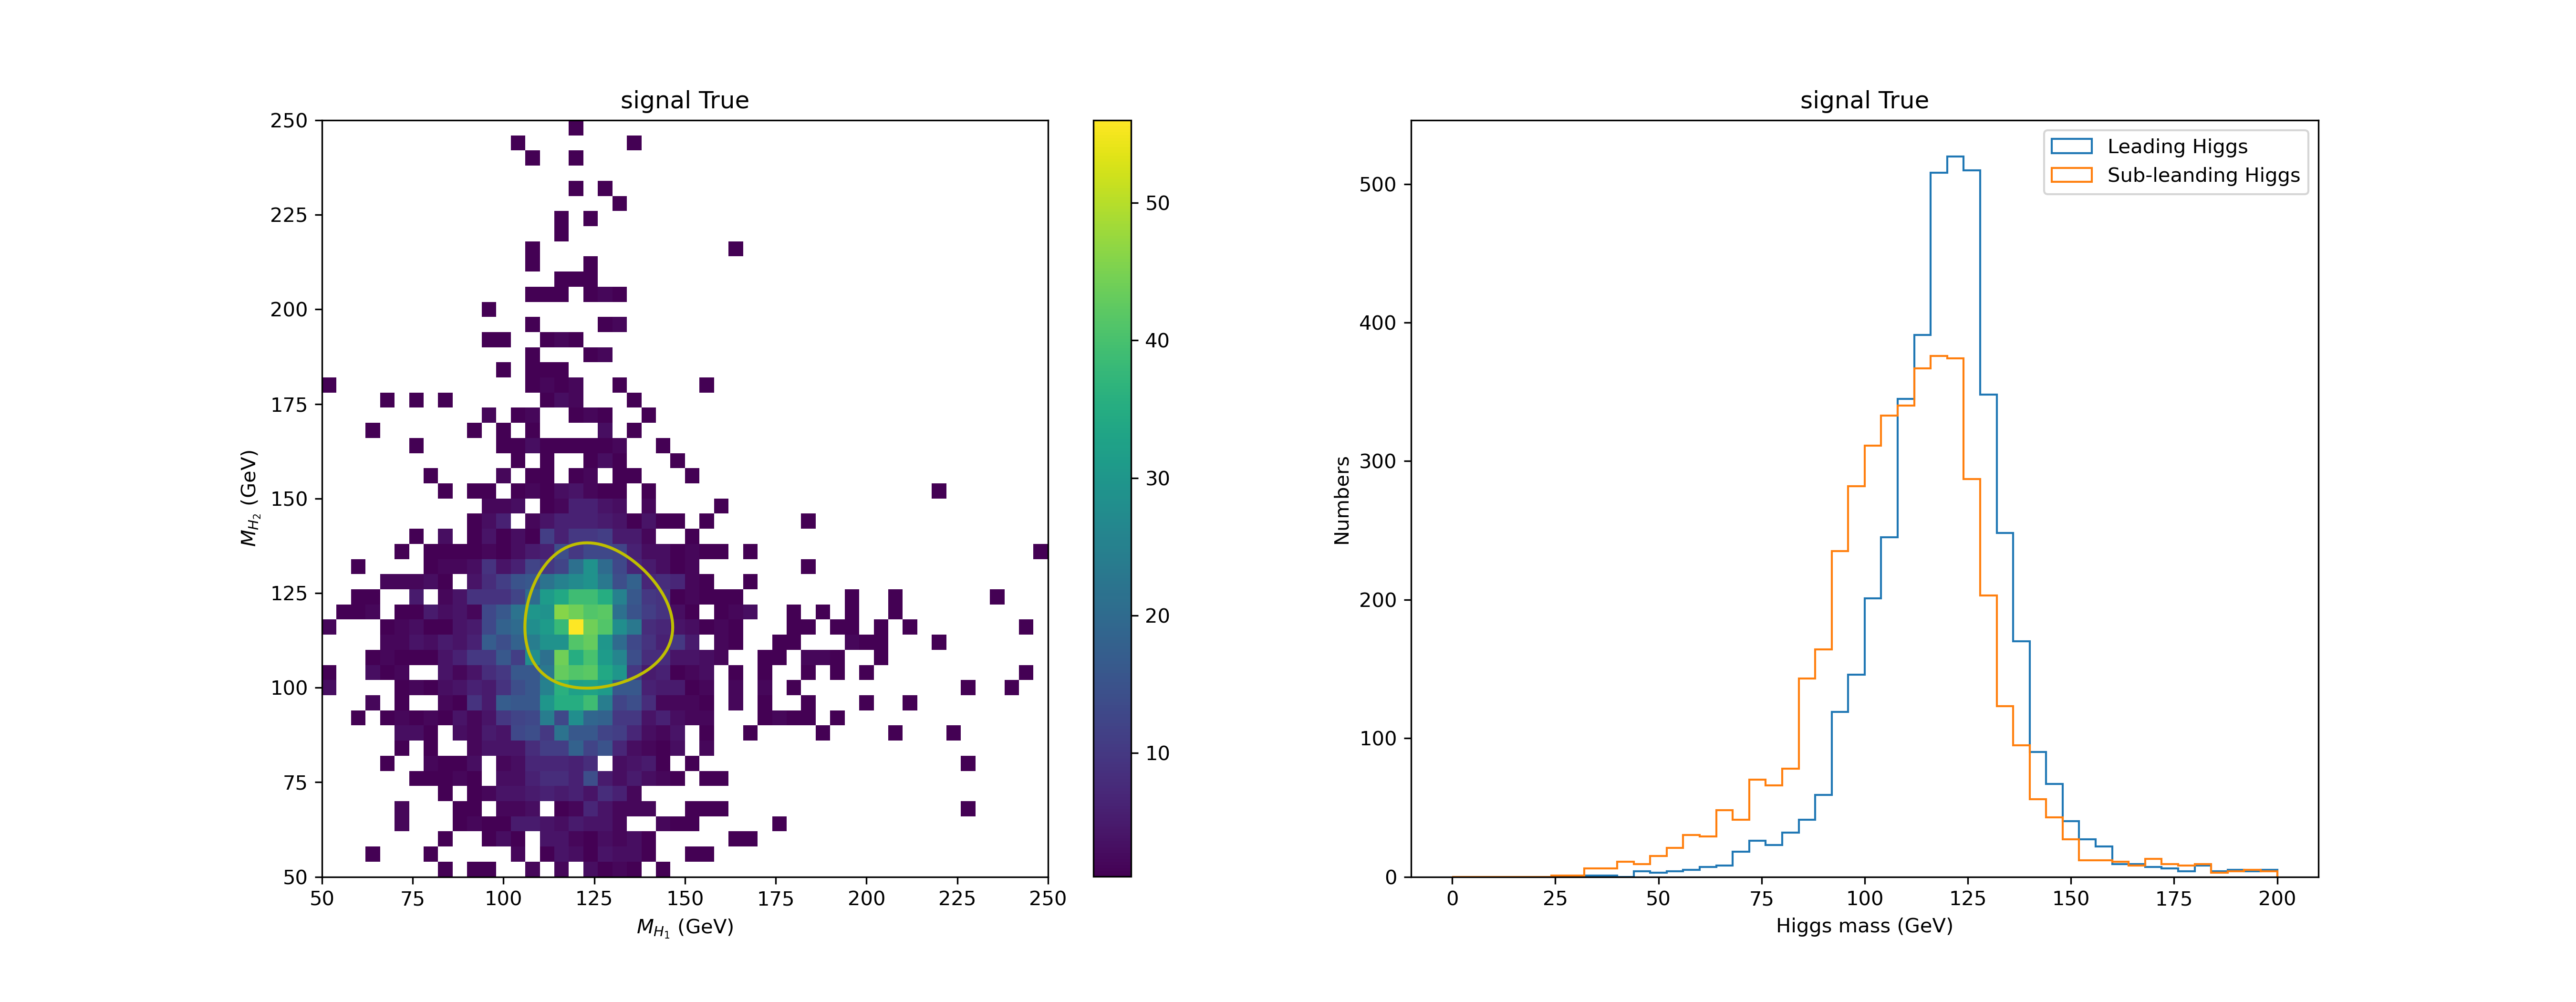
\includegraphics[width=0.97\textwidth]{Higgs_mass_new_truth_s.png}
			\caption{The mass plane and distribution for truth pairing.}
			\label{fig:Higgs_mass_new_truth}
		\end{figure}

% section pairing_performace (end)
\section{Apply SPANET to non-resonant di-Higgs event again}% (fold)
\label{sec:apply_spanet_to_non_resonant_di_higgs_event_again}
	The bugs for Sec.\ref{sec:apply_spanet_on_non_resonant_di_higgs_event}: Some variables are misdefined twice, so they will get an incorrect number when calculating some physical quantities. 

	Fix this bug, then the cutflow tables for signal and background are in Table \ref{tab:signal_selection_efficiency_SPANet_correct}, \ref{tab:signal_selection_efficiency_background_SPANet_correct}.
	\begin{table}[htpb]
			\centering
			\caption{The selection passing rate and efficiency at each stage for ``$\text{min-}\Delta R$'' and SPA-NET pairing.}
			\label{tab:signal_selection_efficiency_SPANet_correct}
			\begin{tabular}{l|cc|cc|cc}
					& \multicolumn{4}{c|}{$\text{min-}\Delta R$}                               & \multicolumn{2}{c}{SPA-NET}   \\
							  & \multicolumn{2}{c|}{ATLAS} & \multicolumn{2}{c|}{My sample}             & \multicolumn{2}{c}{My sample} \\
				Cut           & pass rate   & efficiency  & pass rate & \multicolumn{1}{c|}{efficiency} & pass rate     & efficiency    \\ \hline
				Four tag      & 0.0649 & 0.0649 & 0.0852 & 0.0852 & 0.0852 & 0.0852\\
				Higgs Eta     & 0.0543 & 0.8360 & 0.0688 & 0.8074 & 0.0676 & 0.7942\\
				Top veto      & 0.0456 & 0.8401 & 0.0553 & 0.8044 & 0.0544 & 0.8051\\
				Signal region & 0.0220 & 0.4818 & 0.0181 & 0.3283 & 0.0194 & 0.3567\\
			\end{tabular}
		\end{table}
		\begin{table}[htpb]
			\centering
			\caption{The selection passing rate and efficiency at each stage for ``$\text{min-}\Delta R$'' and SPA-NET pairing. }
			\label{tab:signal_selection_efficiency_background_SPANet_correct}
			\begin{tabular}{l|cc|cc}
							  & \multicolumn{4}{c}{pp4b}                                                         \\
							  & \multicolumn{2}{c|}{$\text{min-}\Delta R$}& \multicolumn{2}{c}{SPA-NET} \\
				Cut           & pass rate               & efficiency                & pass rate    & efficiency   \\ \hline
				Four tag      & 0.0096                  & 0.0096                    & 0.0096       & 0.0096       \\
				Higgs Eta     & 0.0056                  & 0.5835                    & 0.0050       & 0.5202       \\
				Top veto      & 0.0042                  & 0.7423                    & 0.0037       & 0.7341      \\
				Signal region & 0.0001                  & 0.0232                    & 0.0002       & 0.0443       \\
			\end{tabular}
		\end{table}

		Figure \ref{fig:Higgs_mass_new_SPANET} shows the Higgs mass distribution for SPA-NET pairing.
		\begin{figure}[htpb]
			\centering
			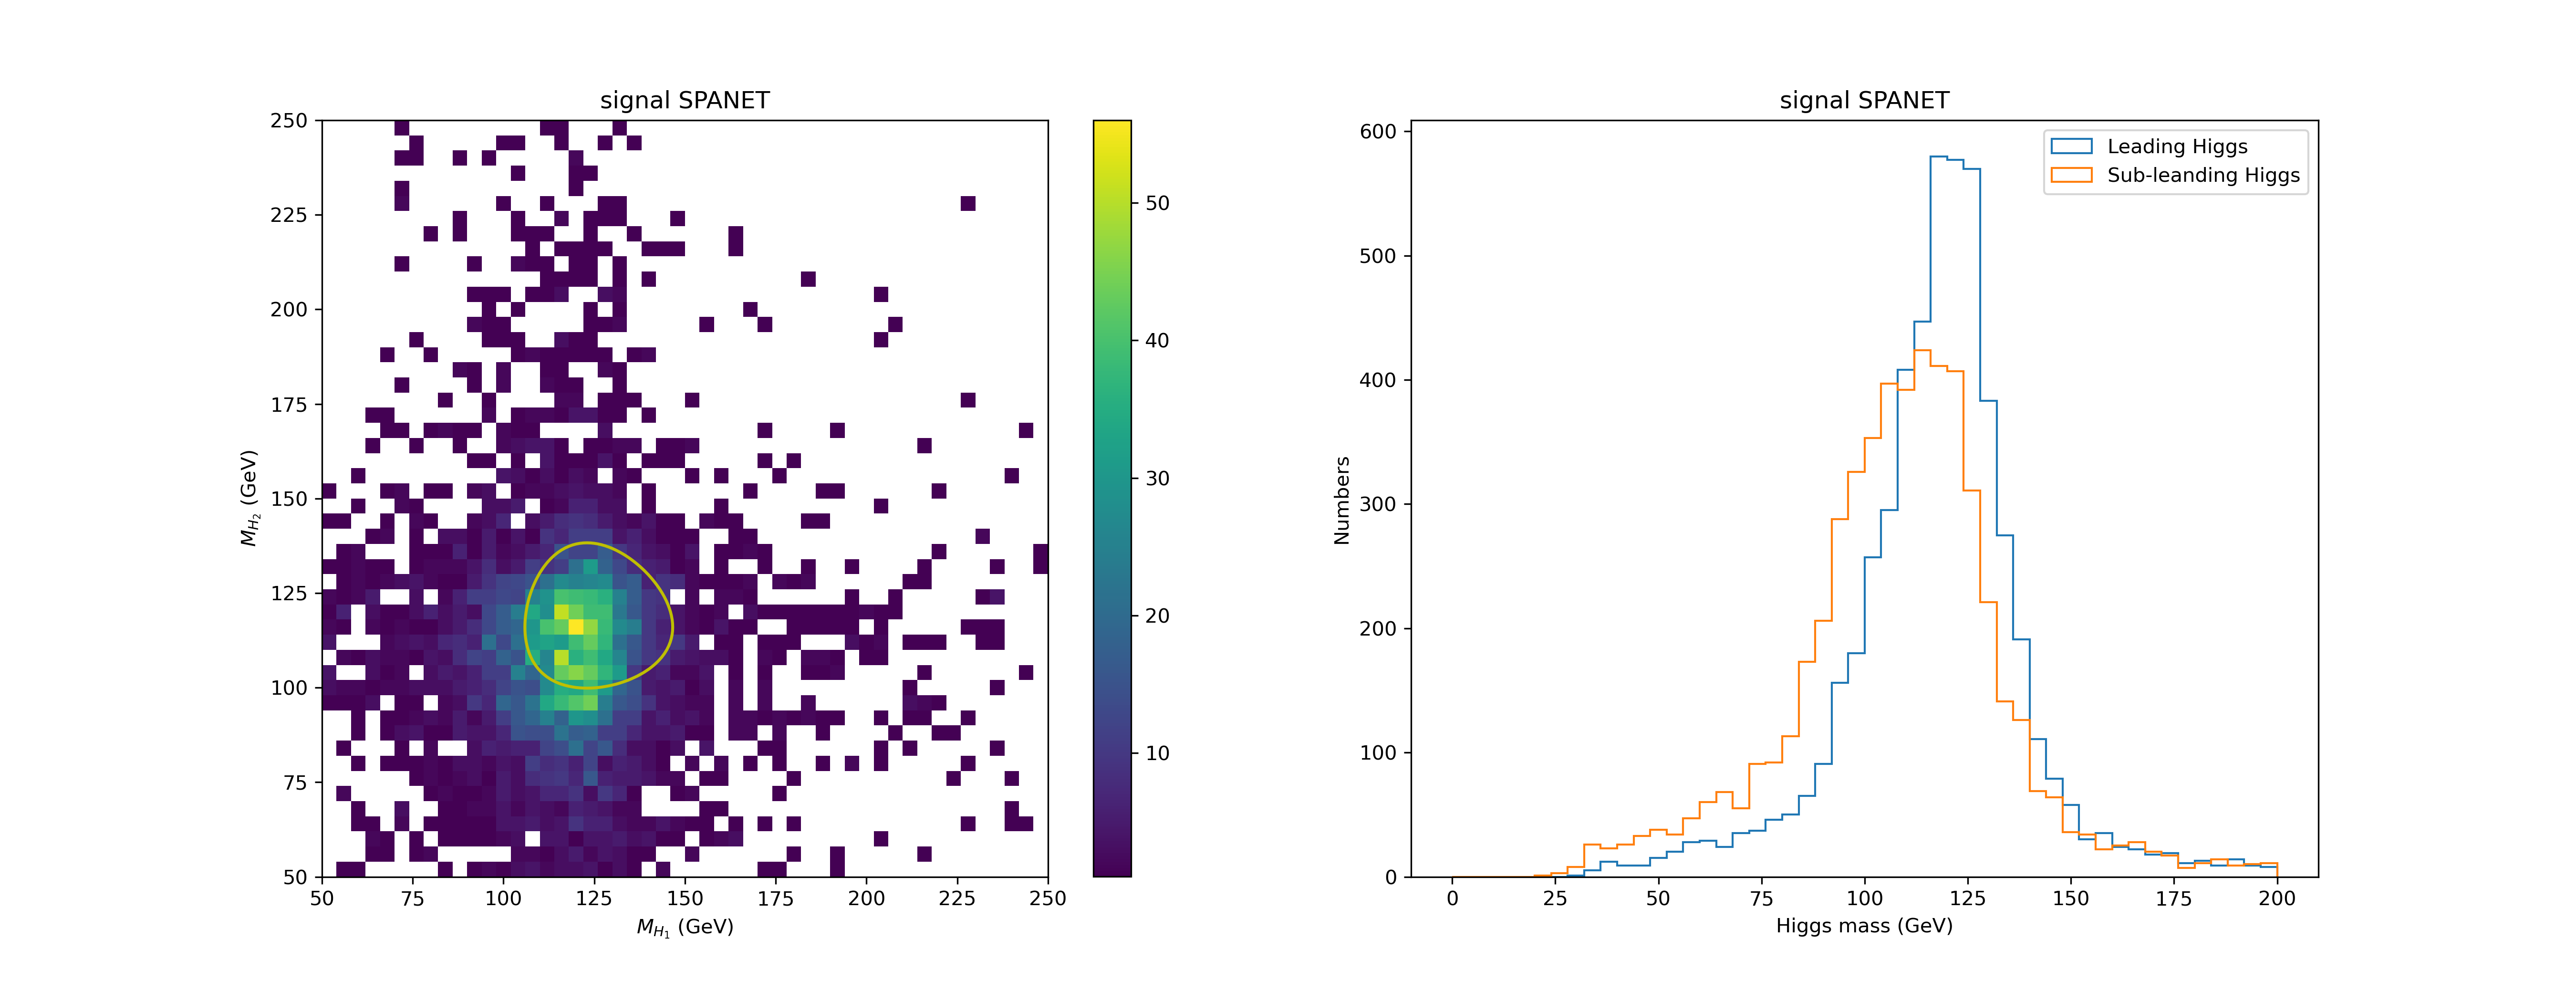
\includegraphics[width=0.97\textwidth]{Higgs_mass_new_SPANET_s.png}
			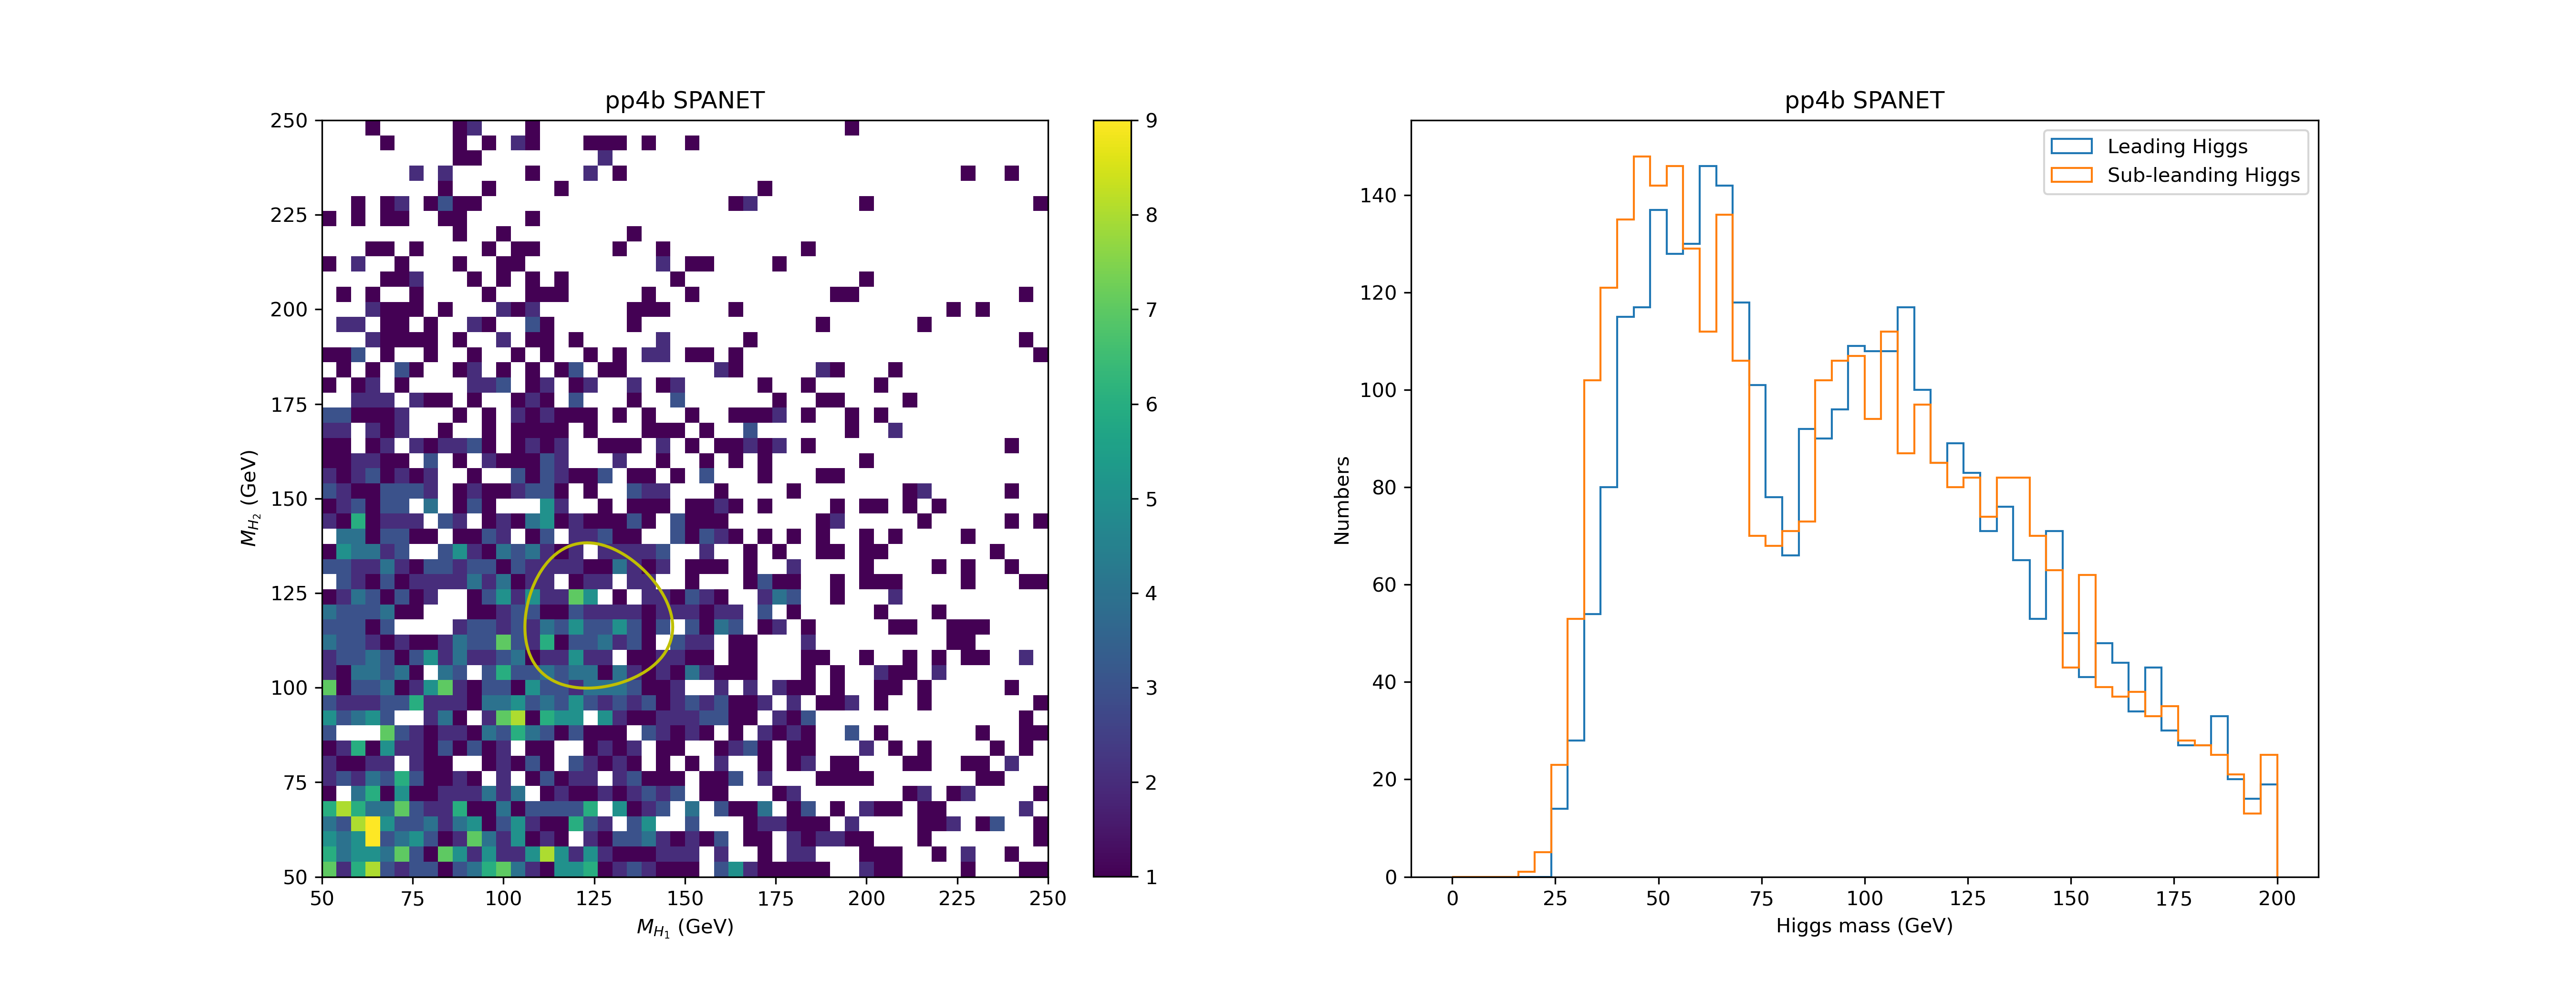
\includegraphics[width=0.97\textwidth]{Higgs_mass_new_SPANET_4b.png}
			\caption{The mass plane and distribution for Higgs candidate for SPA-NET pairing method. The above figure is for the signal sample and the below one is for the background sample.}
			\label{fig:Higgs_mass_new_SPANET}
		\end{figure}

		The ``$\text{min-}\Delta R$'' result is in Table \ref{tab:diHiggs_signal_background_analysis_ATLAS_mindR}. The SPANet result is in Table \ref{tab:diHiggs_signal_background_analysis_ATLAS_SPANet}.

		The SPA-NET method will let more signal events pass the Higgs signal cut, but also true for the background process. Therefore, the SPA-NET pairing method can not improve the $S/\sqrt{B}$.
		\begin{table}[htpb]
			\centering
			\caption{The cross sections for the di-Higgs signal and background processes at different cuts. The pairing method is ``$\text{min-}\Delta R$''.}
			\label{tab:diHiggs_signal_background_analysis_ATLAS_mindR}
			\begin{tabular}{l|cc|c|c|c|c}
							 & \multicolumn{2}{c|}{Cross section (fb)} &          & $\mathcal{L} = 139 \text{ fb}^{-1}$ & $\mathcal{L} = 300 \text{ fb}^{-1}$ & $\mathcal{L} = 3000 \text{ fb}^{-1}$ \\
							 & Signal           & Background           & $S / B$  & $S/\sqrt{B}$                        & $S/\sqrt{B}$                        & $S/\sqrt{B}$                         \\ \hline
				No cut       & 6.774 & 6.29e+05 & 1.08e-05 & 0.101  & 0.148 & 0.468 \\
				Four tag     & 0.577 & 6.06e+03 & 9.52e-05 & 0.0874 & 0.128 & 0.406 \\
				Higgs Eta    & 0.466 & 3.54e+03 & 0.000132 & 0.0923 & 0.136 & 0.429 \\
				Top veto     & 0.375 & 2.62e+03 & 0.000143 & 0.0862 & 0.127 & 0.401 \\
				Higgs signal & 0.123 & 61.0     & 0.00202  & 0.186  & 0.273 & 0.862
			\end{tabular}	
		\end{table}

		\begin{table}[htpb]
			\centering
			\caption{The cross sections for the di-Higgs signal and background processes at different cuts. The pairing method is SPA-NET.}
			\label{tab:diHiggs_signal_background_analysis_ATLAS_SPANet}
			\begin{tabular}{l|cc|c|c|c|c}
							 & \multicolumn{2}{c|}{Cross section (fb)} &          & $\mathcal{L} = 139 \text{ fb}^{-1}$ & $\mathcal{L} = 300 \text{ fb}^{-1}$ & $\mathcal{L} = 3000 \text{ fb}^{-1}$ \\
							 & Signal           & Background           & $S / B$  & $S/\sqrt{B}$                        & $S/\sqrt{B}$                        & $S/\sqrt{B}$                         \\ \hline
				No cut       & 6.774 & 6.29e+05 & 1.08e-05 & 0.101  & 0.148 & 0.468 \\
				Four tag     & 0.577 & 6.06e+03 & 9.52e-05 & 0.0874 & 0.128 & 0.406 \\
				Higgs Eta    & 0.458 & 3.15e+03 & 0.000145 & 0.0962 & 0.141 & 0.447 \\
				Top veto     & 0.369 & 2.31e+03 & 0.000159 & 0.0904 & 0.133 & 0.420 \\
				Higgs signal & 0.132 & 1.02e+02 & 0.00128  & 0.153  & 0.225 & 0.712			
			\end{tabular}
		\end{table}

% section apply_spanet_to_non_resonant_di_higgs_event_again (end)		
\section{Train on resonant test on SM}% (fold)
\label{sec:train_on_resonant_test_on_sm}
	In Figure \ref{fig:di-Higgs-SM-kappa-mhh}, there is a peak around $\text{450 GeV}$ in the SM ($\kappa_\lambda = 1$) $m_{hh}$ distribution. This section trains a SPA-NET on the resonant samples with resonant mass $\text{450 GeV}$, then test its performance on SM samples.

	\subsection{SPA-NET training on 450 GeV}% (fold)
	\label{sub:spa_net_training_on_450_gev}
		Set $m_H = \text{450 GeV}$. The training samples are required to pass the ``Four tag cut'', i.e., there are at least four b-tagged jets with $p_{\text{T}} > \text{40 GeV}$ and $\abs{\eta} < 2.5$.
		\begin{itemize}
			\item Training sample:
			\begin{itemize}
				\item Total sample size: 51,145
				\item 1h sample size: 9,320
				\item 2h sample size: 40,991
				\item 5\% used on validation
			\end{itemize}
			\item Testing sample: 
			\begin{itemize}
				\item Total sample size: 5,683
				\item 1h sample size: 1,011
				\item 2h sample size: 4,582
			\end{itemize}
		\end{itemize}
		The training results are presented in Table \ref{tab:SPANet_diHiggs_4btag_pt40_450GeV}.
		\begin{table}[htpb]
			\centering
			\caption{SPA-NET training results on the resonant di-Higgs samples with ``Four tag cut''.}
			\label{tab:SPANet_diHiggs_4btag_pt40_450GeV}
			\begin{tabular}{c|c|cc}
				$N_\text{Jet}$ & Event Fraction & Event Efficiency & Higgs Efficiency \\
				\hline
				$=4$	  &   0.316             &    0.992              &    0.992             \\
				$=5$	  &   0.282             &    0.903              &    0.936             \\
				$\ge 6$	  &   0.208             &    0.768              &    0.838             \\
				Total	  &   0.806             &    0.903              &    0.933             \\
			\end{tabular}
		\end{table}

	% subsection spa_net_training_on_450_gev (end)
	\subsection{Test SPA-NET on SM event}% (fold)
	\label{sub:test_spa_net_on_sm_event}
		In the below, the SPA-NET trained in Sec.\ref{sub:spa_net_training_on_450_gev} is called ``resonant SPA-NET''. Test the resonant SPA-NET on the non-resonant events. The testing results are in Table \ref{tab:SPANet_train_450GeV_test_SM}. The event efficiency is $0.805$. This result is worse than ``train on resonant test on resonant $0.903$'' and ``train on SM test on SM $0.868$''.
		\begin{table}[htpb]
			\centering
			\caption{SPA-NET testing results on the non-resonant di-Higgs samples. Where the SPA-NET is trained on the resonant samples.}
			\label{tab:SPANet_train_450GeV_test_SM}
			\begin{tabular}{c|c|cc}
				$N_\text{Jet}$ & Event Fraction & Event Efficiency & Higgs Efficiency \\
				\hline
				$=4$	  &   0.280             &    0.940              &    0.940             \\
				$=5$	  &   0.287             &    0.790              &    0.861             \\
				$\ge 6$	  &   0.229             &    0.649              &    0.756             \\
				Total	  &   0.797             &    0.805              &    0.861             \\
			\end{tabular}
		\end{table}
	% subsection test_spa_net_on_sm_event (end)
	\subsection{Apply the resonant SPA-NET on SM pairing}% (fold)
	\label{sub:apply_the_resonant_spa_net_on_sm_pairing}
		The ``$ \text{min-}\Delta R$'' pairing is replaced by SPA-NET pairing. Other cuts remained unchanged. The cutflow tables for signal and background are in Table \ref{tab:signal_selection_efficiency_resonant_SPANET}, \ref{tab:signal_selection_efficiency_background_resonant_SPANET}.
		\begin{table}[htpb]
			\centering
			\caption{The selection passing rate and efficiency at each stage for ``$\text{min-}\Delta R$'' and SPA-NET pairing. The SPA-NET is trained in Sec.\ref{sub:spa_net_training_on_450_gev}}
			\label{tab:signal_selection_efficiency_resonant_SPANET}
			\begin{tabular}{l|cc|cc|cc}
					& \multicolumn{4}{c|}{$\text{min-}\Delta R$}                               & \multicolumn{2}{c}{SPA-NET}   \\
							  & \multicolumn{2}{c|}{ATLAS} & \multicolumn{2}{c|}{My sample}             & \multicolumn{2}{c}{My sample} \\
				Cut           & pass rate   & efficiency  & pass rate & \multicolumn{1}{c|}{efficiency} & pass rate     & efficiency    \\ \hline
				Four tag      & 0.0649 & 0.0649 & 0.0852 & 0.0852 & 0.0852 & 0.0852\\
				Higgs Eta     & 0.0543 & 0.8360 & 0.0688 & 0.8074 & 0.0685 & 0.8022\\
				Top veto      & 0.0456 & 0.8401 & 0.0553 & 0.8044 & 0.0550 & 0.8048\\
				Signal region & 0.0220 & 0.4818 & 0.0181 & 0.3283 & 0.0181 & 0.3296\\
			\end{tabular}
		\end{table}
		\begin{table}[htpb]
			\centering
			\caption{The selection passing rate and efficiency at each stage for ``$\text{min-}\Delta R$'' and SPA-NET pairing. The SPA-NET is trained in Sec.\ref{sub:spa_net_training_on_450_gev}}
			\label{tab:signal_selection_efficiency_background_resonant_SPANET}
			\begin{tabular}{l|cc|cc}
							  & \multicolumn{4}{c}{pp4b}                                                         \\
							  & \multicolumn{2}{c|}{$\text{min-}\Delta R$}& \multicolumn{2}{c}{SPA-NET} \\
				Cut           & pass rate               & efficiency                & pass rate    & efficiency   \\ \hline
				Four tag      & 0.0096                  & 0.0096                    & 0.0096       & 0.0096       \\
				Higgs Eta     & 0.0056                  & 0.5835                    & 0.0054       & 0.5589       \\
				Top veto      & 0.0042                  & 0.7423                    & 0.0039       & 0.7326      \\
				Signal region & 0.0001                  & 0.0232                    & 0.0001       & 0.0200       \\
			\end{tabular}
		\end{table}

		Figure \ref{fig:Higgs_mass_new_resonant_SPANET} shows the Higgs mass distribution for resonant SPA-NET pairing.
		\begin{figure}[htpb]
			\centering
			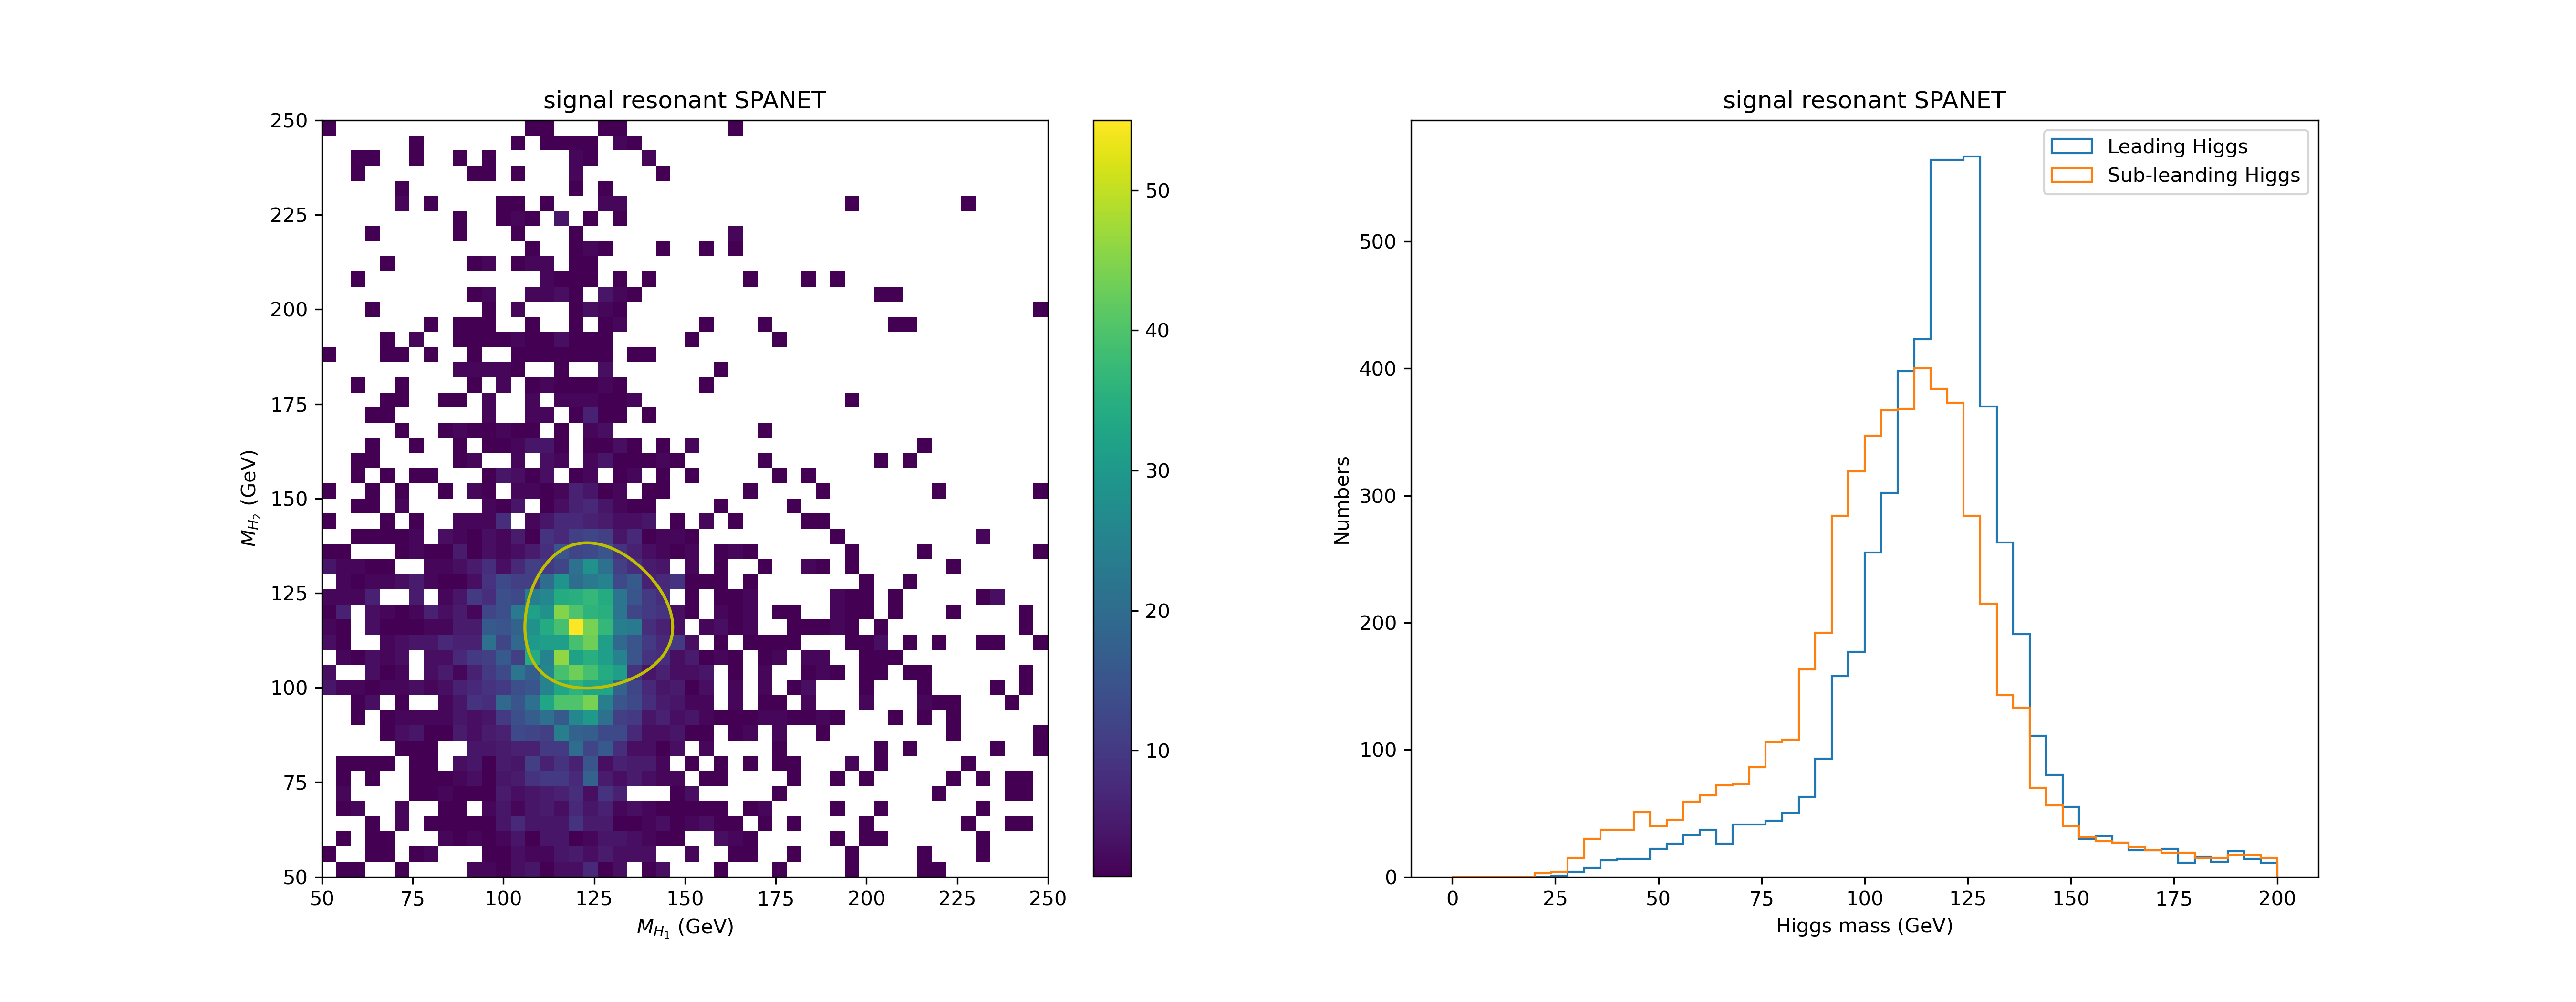
\includegraphics[width=0.97\textwidth]{Higgs_mass_new_res-SPANET_s.png}
			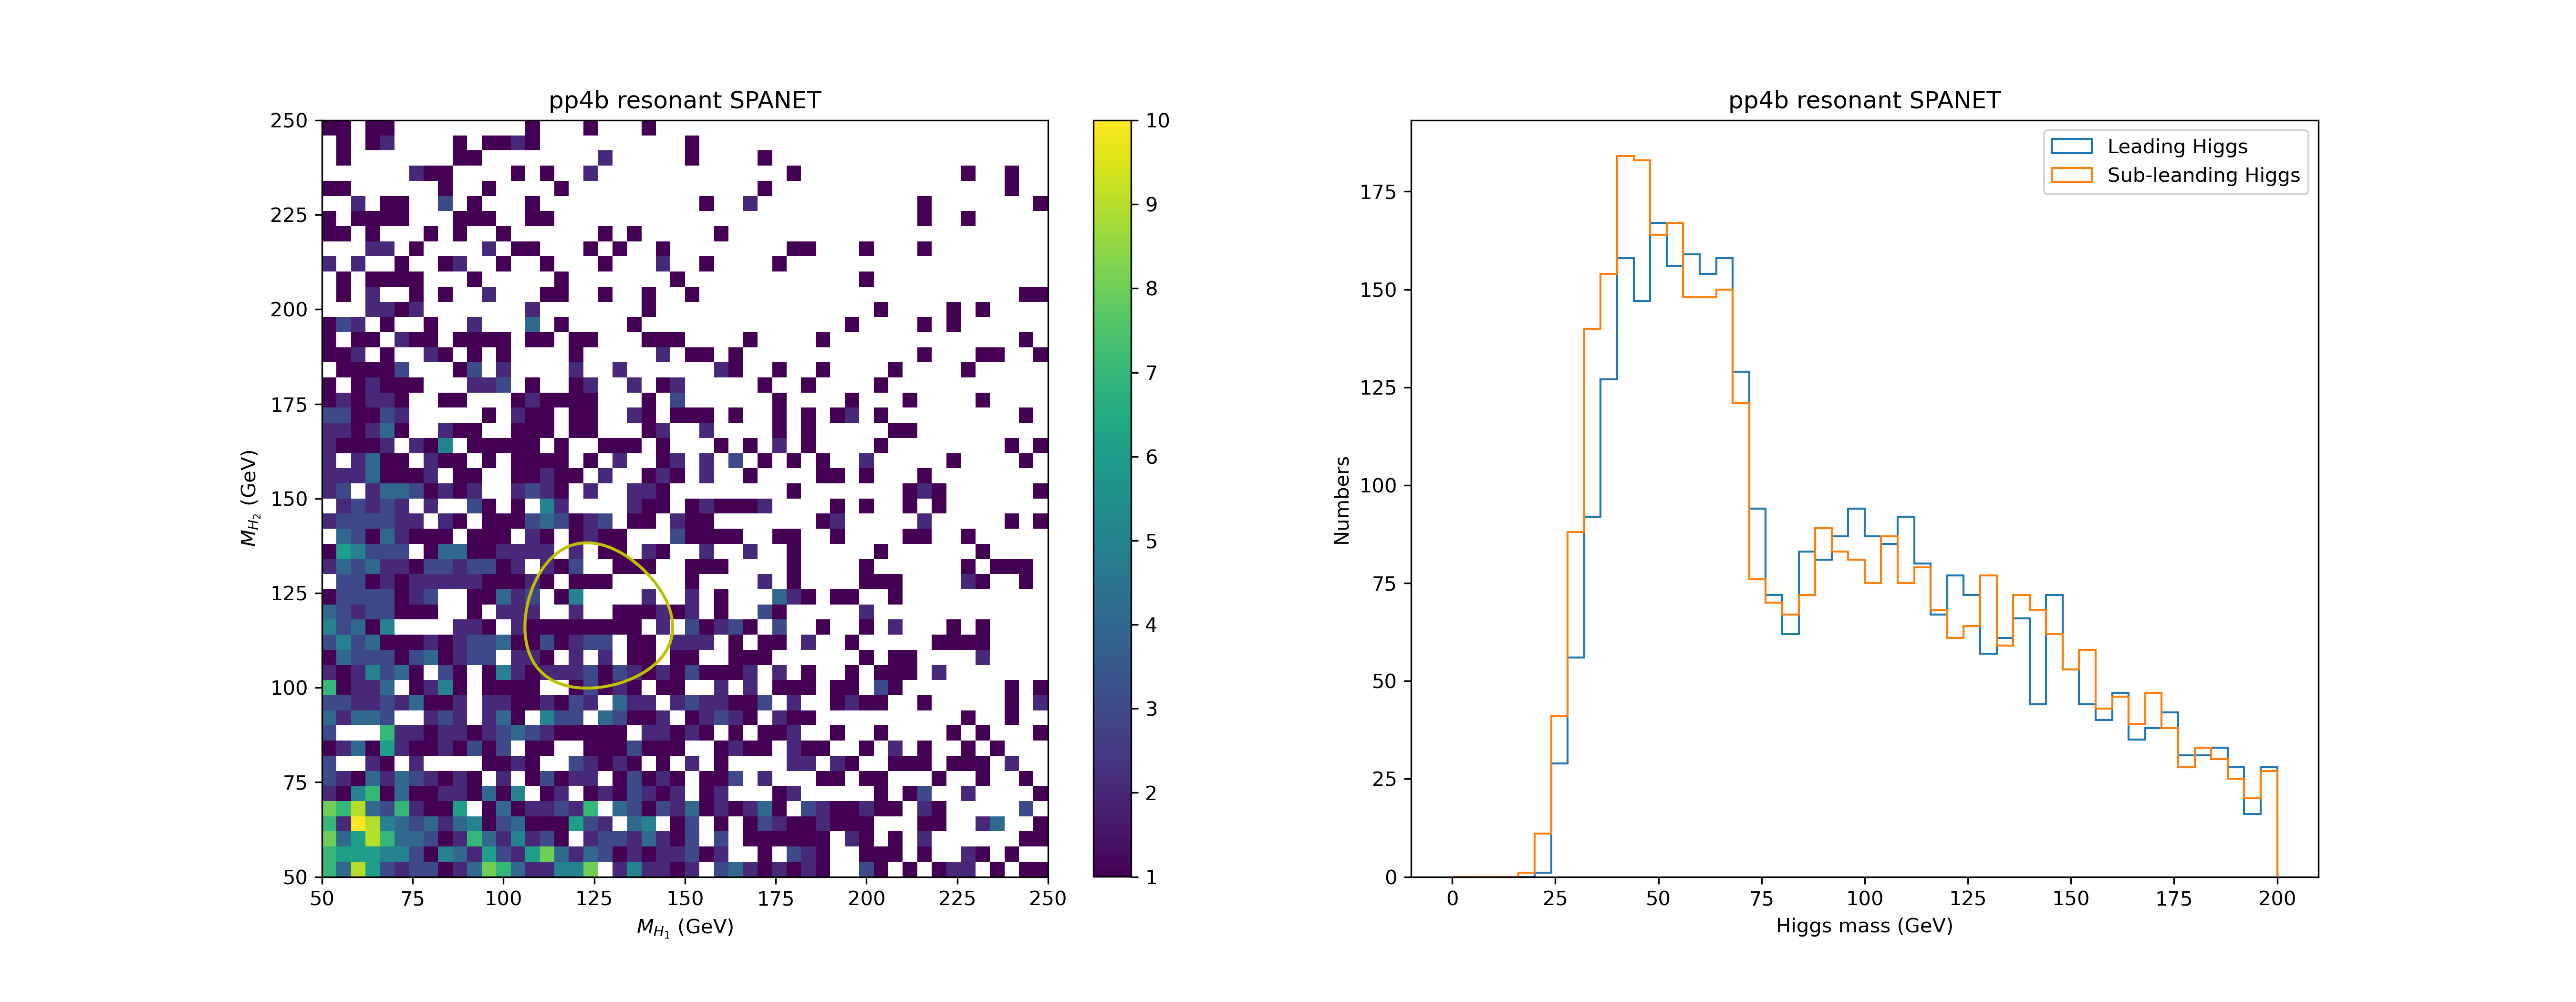
\includegraphics[width=0.97\textwidth]{Higgs_mass_new_res-SPANET_4b.png}
			\caption{The mass plane and distribution for Higgs candidate for resonant SPA-NET pairing. The above figure is for the signal sample and the below one is for the background sample.}
			\label{fig:Higgs_mass_new_resonant_SPANET}
		\end{figure}
		The $\frac{S}{\sqrt{B}}$ of resonant SPA-NET results are in Table \ref{tab:diHiggs_signal_background_analysis_ATLAS_resonant_SPANET}.

		Compared to ``$\text{min-}\Delta R$'' method (Table \ref{tab:diHiggs_signal_background_analysis_ATLAS_mindR}), the resonant SPA-NET will let roughly the same number of signal events pass the Higgs signal cut, and let the smaller number of the background events pass, but not so much difference. Therefore, the resonant SPA-NET can a little improve the $S/\sqrt{B}$.

		\begin{table}[htpb]
			\centering
			\caption{The cross sections for the di-Higgs signal and background processes at different cuts. The pairing method is resonant SPA-NET. Compared to Table \ref{tab:diHiggs_signal_background_analysis_ATLAS_mindR}, there is a little improvement.}
			\label{tab:diHiggs_signal_background_analysis_ATLAS_resonant_SPANET}
			\begin{tabular}{l|cc|c|c|c|c}
							 & \multicolumn{2}{c|}{Cross section (fb)} &          & $\mathcal{L} = 139 \text{ fb}^{-1}$ & $\mathcal{L} = 300 \text{ fb}^{-1}$ & $\mathcal{L} = 3000 \text{ fb}^{-1}$ \\
							 & Signal           & Background           & $S / B$  & $S/\sqrt{B}$                        & $S/\sqrt{B}$                        & $S/\sqrt{B}$                         \\ \hline
				No cut       & 6.774 & 6.29e+05 & 1.08e-05 & 0.101  & 0.148 & 0.468 \\
				Four tag     & 0.577 & 6.06e+03 & 9.52e-05 & 0.0874 & 0.128 & 0.406 \\
				Higgs Eta    & 0.464 & 3.39e+03 & 0.000137 & 0.0941 & 0.138 & 0.437 \\
				Top veto     & 0.372 & 2.48e+03 & 0.00015  & 0.0881 & 0.129 & 0.410 \\
				Higgs signal & 0.123 & 49.7     & 0.00247  & 0.205  & 0.302 & 0.954	
			\end{tabular}
		\end{table}

	% subsection apply_the_resonant_spa_net_on_sm_pairing (end)	
% section train_on_resonant_test_on_sm (end)
\section{Apply the \texorpdfstring{$\text{min-}\Delta R$}{min delta R} method on the resonant sample}% (fold)
\label{sec:apply_the_min_delta_r_method_on_the_resonant_sample}
	In the previous, the pairing method for resonant samples is $\Delta R+\text{min-}D_{HH}$ method. This section will test the $\text{min-}\Delta R$ pairing method for resonant samples. The ``$\Delta R + \text{min-}D_{HH}$'' pairing is replaced by $\text{min-}\Delta R$ pairing. Other cuts remained unchanged. The cutflow tables for signal and background are in Table \ref{tab:signal_selection_efficiency_1000GeV_MV2c10_mindR}, \ref{tab:signal_selection_efficiency_background_MV2c10_mindR}.
	\begin{table}[htpb]
		\centering
		\caption{The selection passing rate and efficiency at each stage for $\Delta R + \text{min-}D_{HH}$, $\text{min-}\Delta R$ and SPA-NET pairing. The resonant mass is $\text{1000 GeV}$.}
		\label{tab:signal_selection_efficiency_1000GeV_MV2c10_mindR}
		\begin{tabular}{l|cc|cc|cc}
				 & \multicolumn{2}{c|}{$\Delta R + \text{min-}D_{HH}$} & \multicolumn{2}{c|}{$\text{min-}\Delta R$} & \multicolumn{2}{c}{SPA-NET} \\
			Cut	 & pass rate               & efficiency               & pass rate           & efficiency          & pass rate    & efficiency   \\ \hline
			Four tag     & 0.1257 & 0.1257 & 0.1257 & 0.1257 & 0.1257 & 0.1257 \\
			Delta R      & 0.1087 & 0.8644 & N.A.   & N.A.   & N.A.   & N.A.   \\
			Higgs PT     & 0.0896 & 0.8247 & 0.0936 & 0.7444 & 0.0978 & 0.7775 \\
			Higgs Eta    & 0.0826 & 0.9216 & 0.0863 & 0.9226 & 0.0900 & 0.9203 \\
			Higgs signal & 0.0445 & 0.5391 & 0.0445 & 0.5155 & 0.0468 & 0.5197 \\
			Top veto     & 0.0425 & 0.9555 & 0.0425 & 0.9553 & 0.0446 & 0.9536
		\end{tabular}
	\end{table}
	\begin{table}[htpb]
		\centering
		\caption{The selection passing rate and efficiency at each stage for $\Delta R + \text{min-}D_{HH}$, $\text{min-}\Delta R$ and SPA-NET pairing.}
		\label{tab:signal_selection_efficiency_background_MV2c10_mindR}
		\begin{tabular}{l|cc|cc|cc}
			     & \multicolumn{6}{c}{pp4b}                                                         \\
				 & \multicolumn{2}{c|}{$\Delta R + \text{min-}D_{HH}$} & \multicolumn{2}{c|}{$\text{min-}\Delta R$} & \multicolumn{2}{c}{SPA-NET} \\
			Cut	 & pass rate               & efficiency               & pass rate           & efficiency          & pass rate    & efficiency   \\ \hline
			Four tag     & 0.0096 & 0.0096 & 9.6420e-03 & 0.0096 & 9.6420e-03 & 0.0096 \\
			Delta R      & 0.0050 & 0.5234 & 9.6420e-03 & 1.0000 & 9.6420e-03 & 1.0000 \\
			Higgs PT     & 0.0043 & 0.8462 & 6.6460e-03 & 0.6893 & 6.7200e-03 & 0.6970 \\
			Higgs Eta    & 0.0030 & 0.7127 & 5.0040e-03 & 0.7529 & 4.8580e-03 & 0.7229 \\
			Higgs signal & 0.0005 & 0.1551 & 1.1600e-04 & 0.0232 & 7.5000e-05 & 0.0154 \\
			Top veto     & 0.0003 & 0.5975 & 9.4000e-05 & 0.8103 & 6.6000e-05 & 0.8800
		\end{tabular}
	\end{table}

	Figure \ref{fig:Higgs_mass_old_signal} shows the Higgs mass distribution for resonant signal events with different pairing methods. Figure \ref{fig:Higgs_mass_old_background} is for background events with different pairing methods. The mass planes for the signal process all look similar. For background, $\Delta R + \text{min-}D_{HH}$ pairing is much different from the other two methods.
	\begin{figure}[htpb]
		\centering
		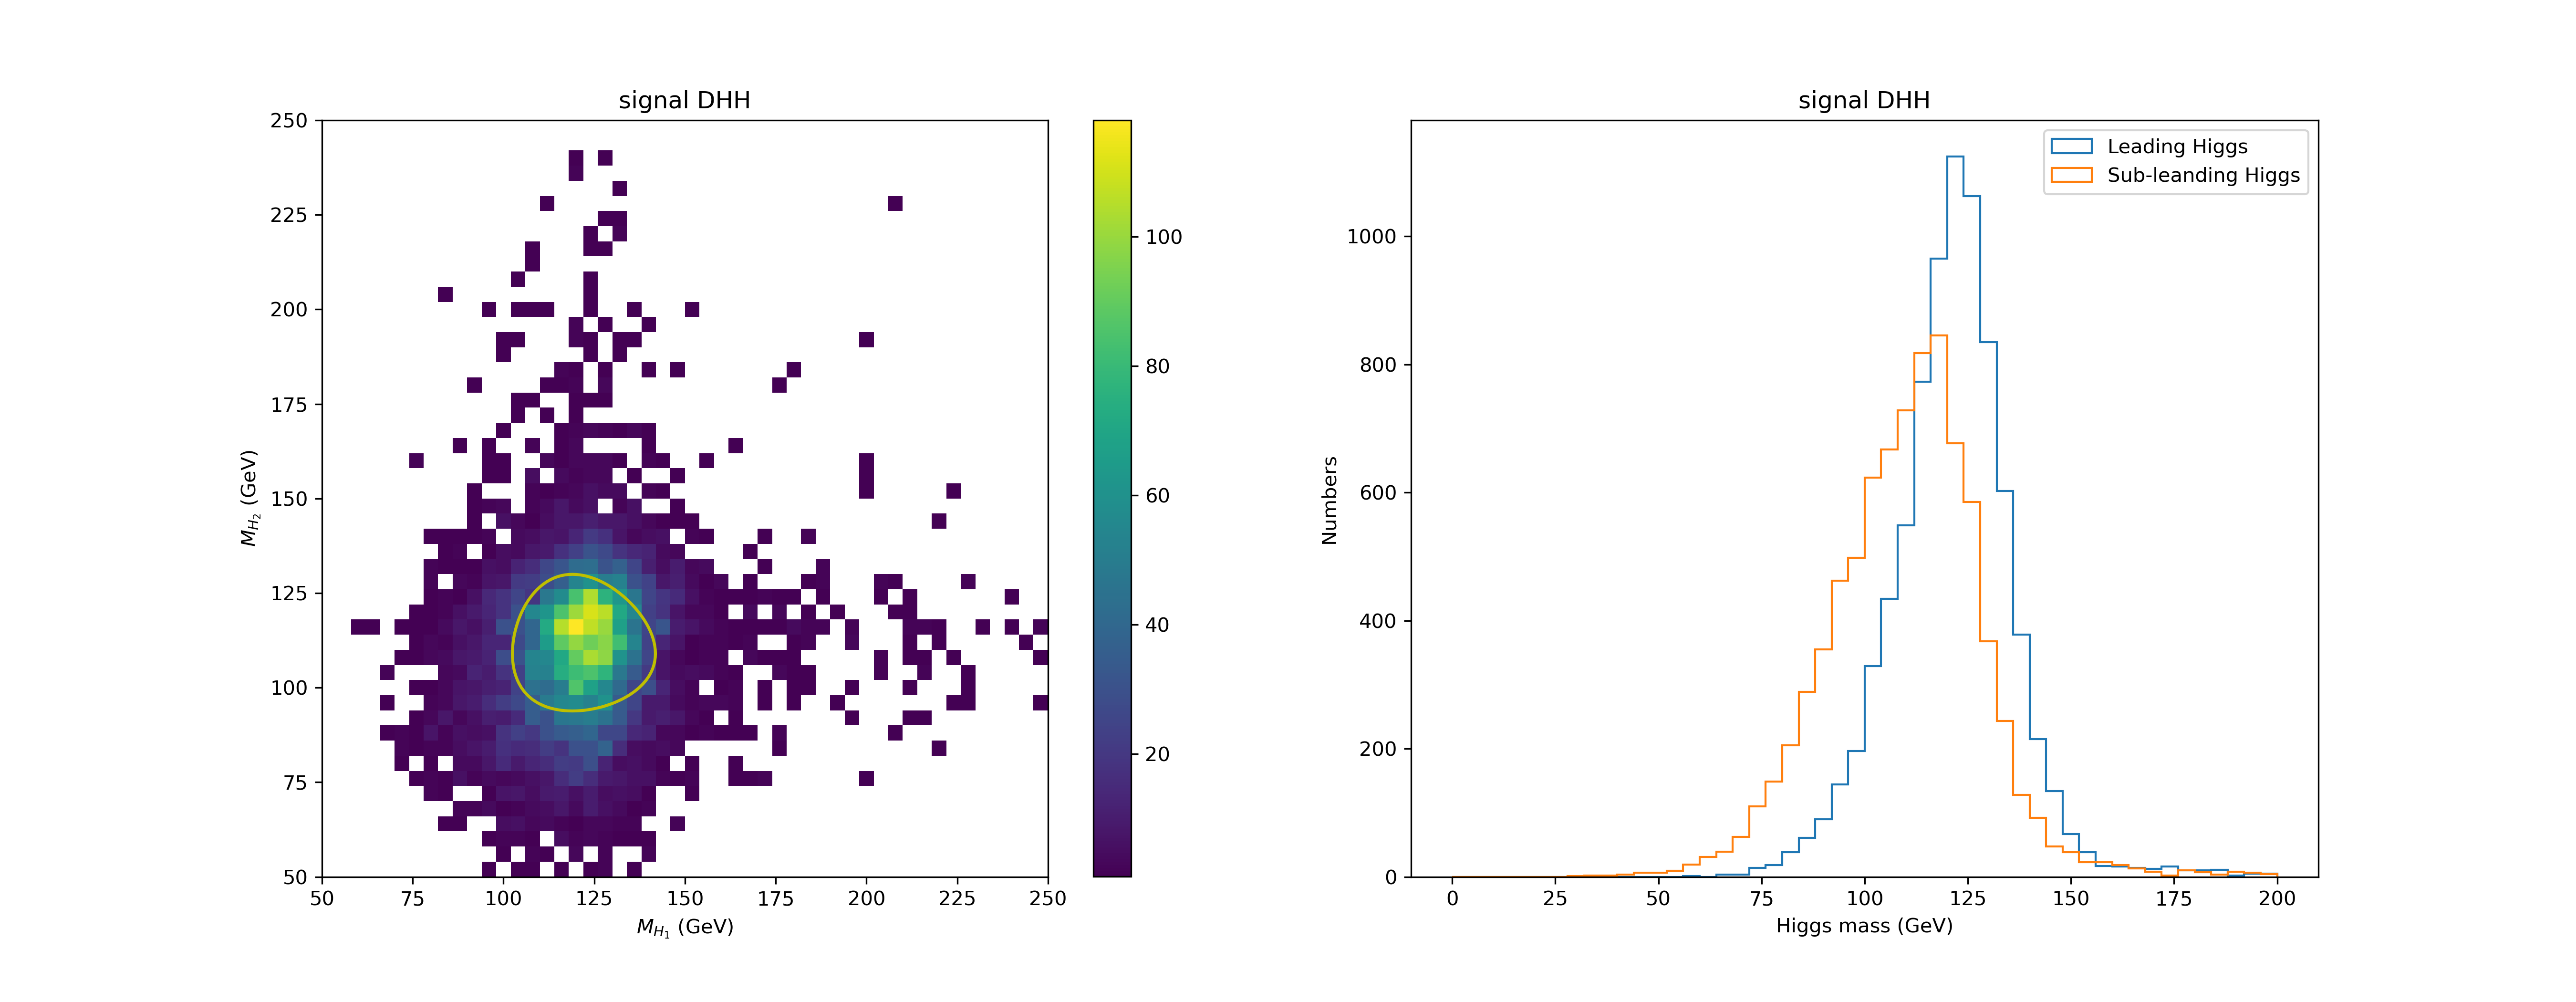
\includegraphics[width=0.97\textwidth]{Higgs_mass_old_DHH_s.png}
		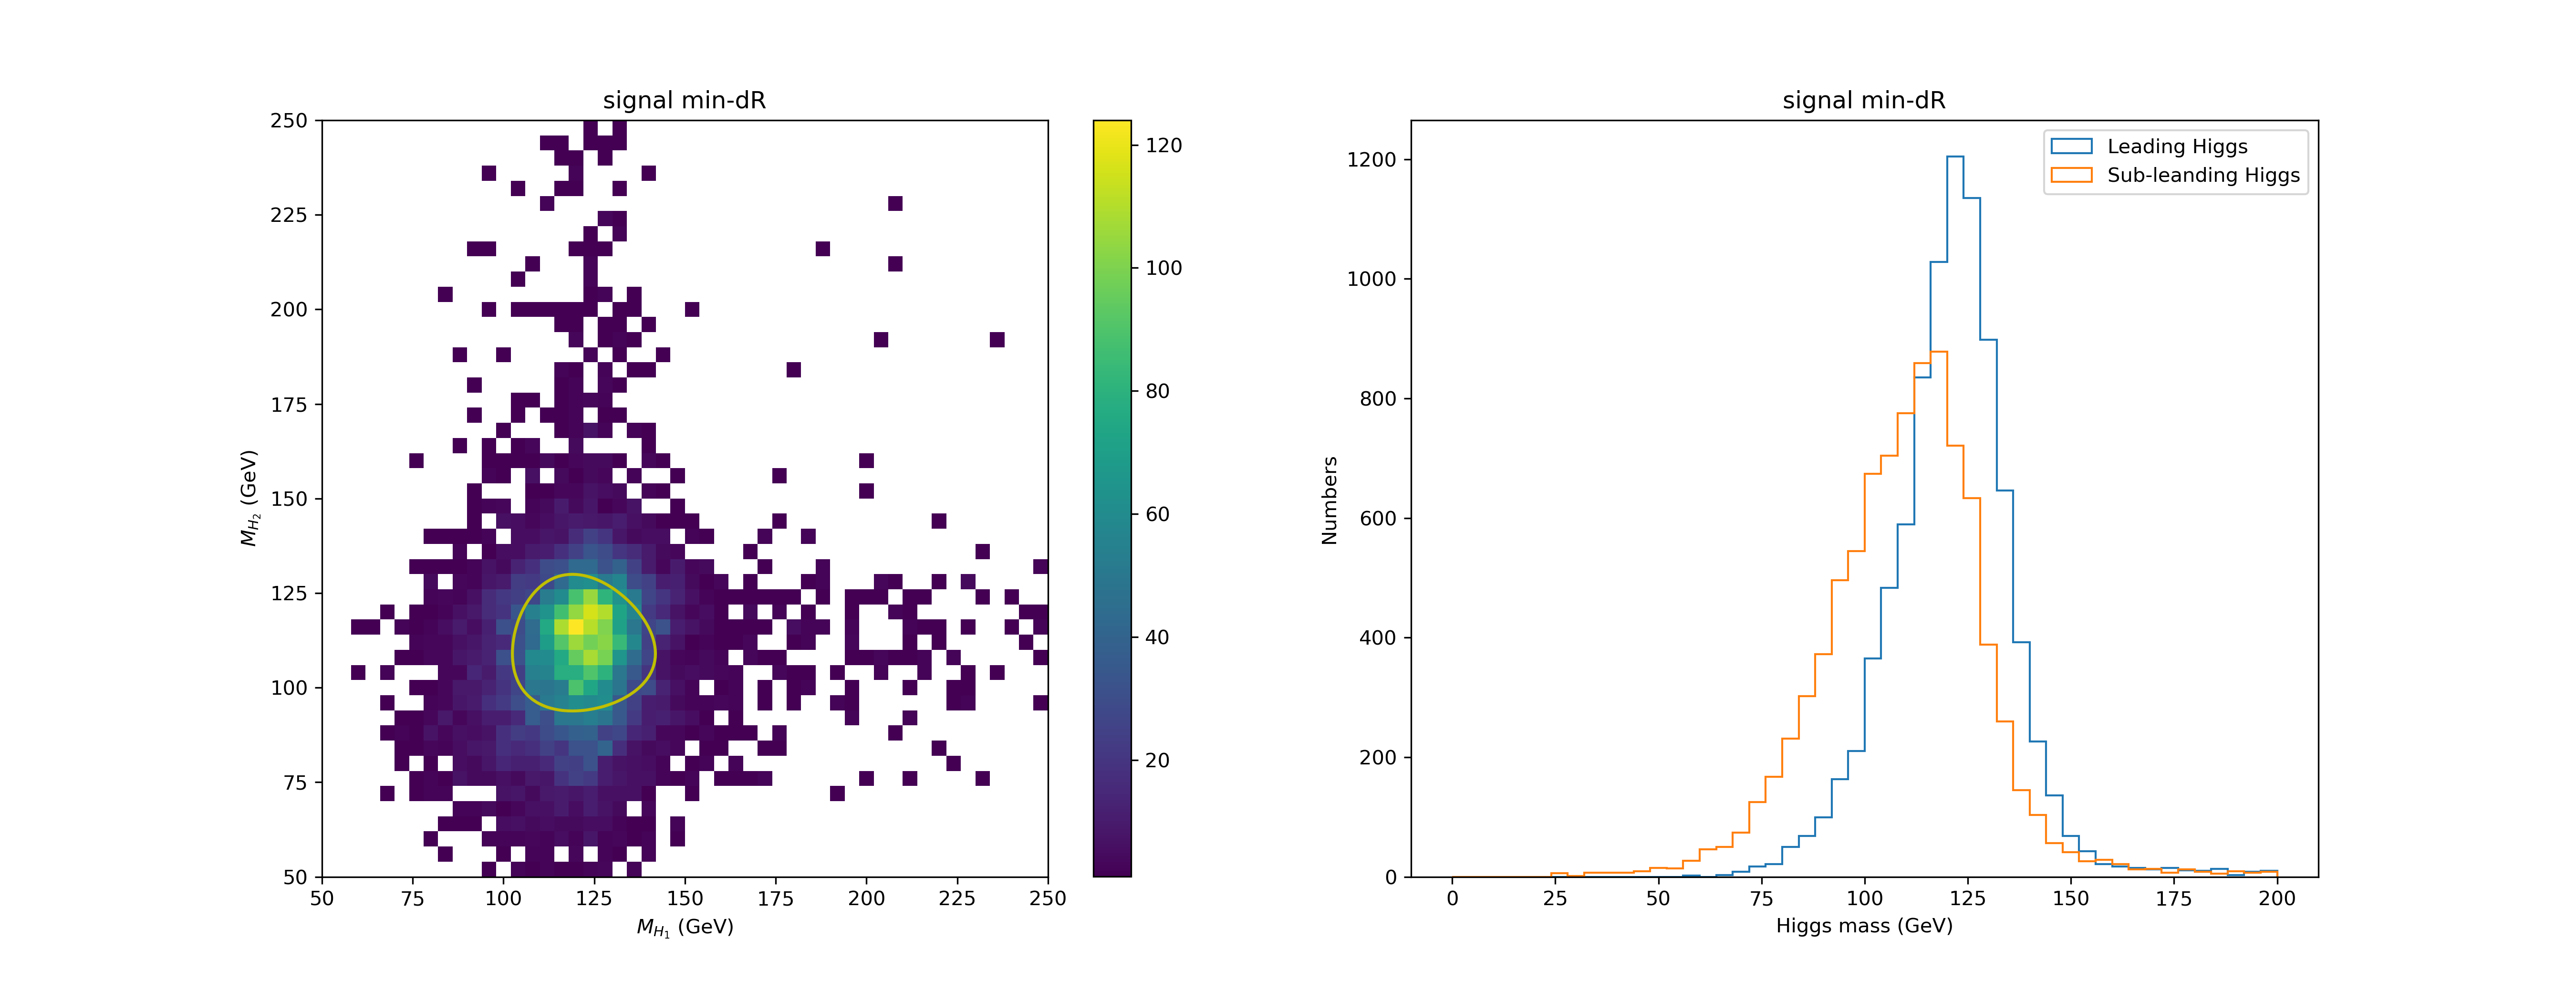
\includegraphics[width=0.97\textwidth]{Higgs_mass_old_mindR_s.png}
		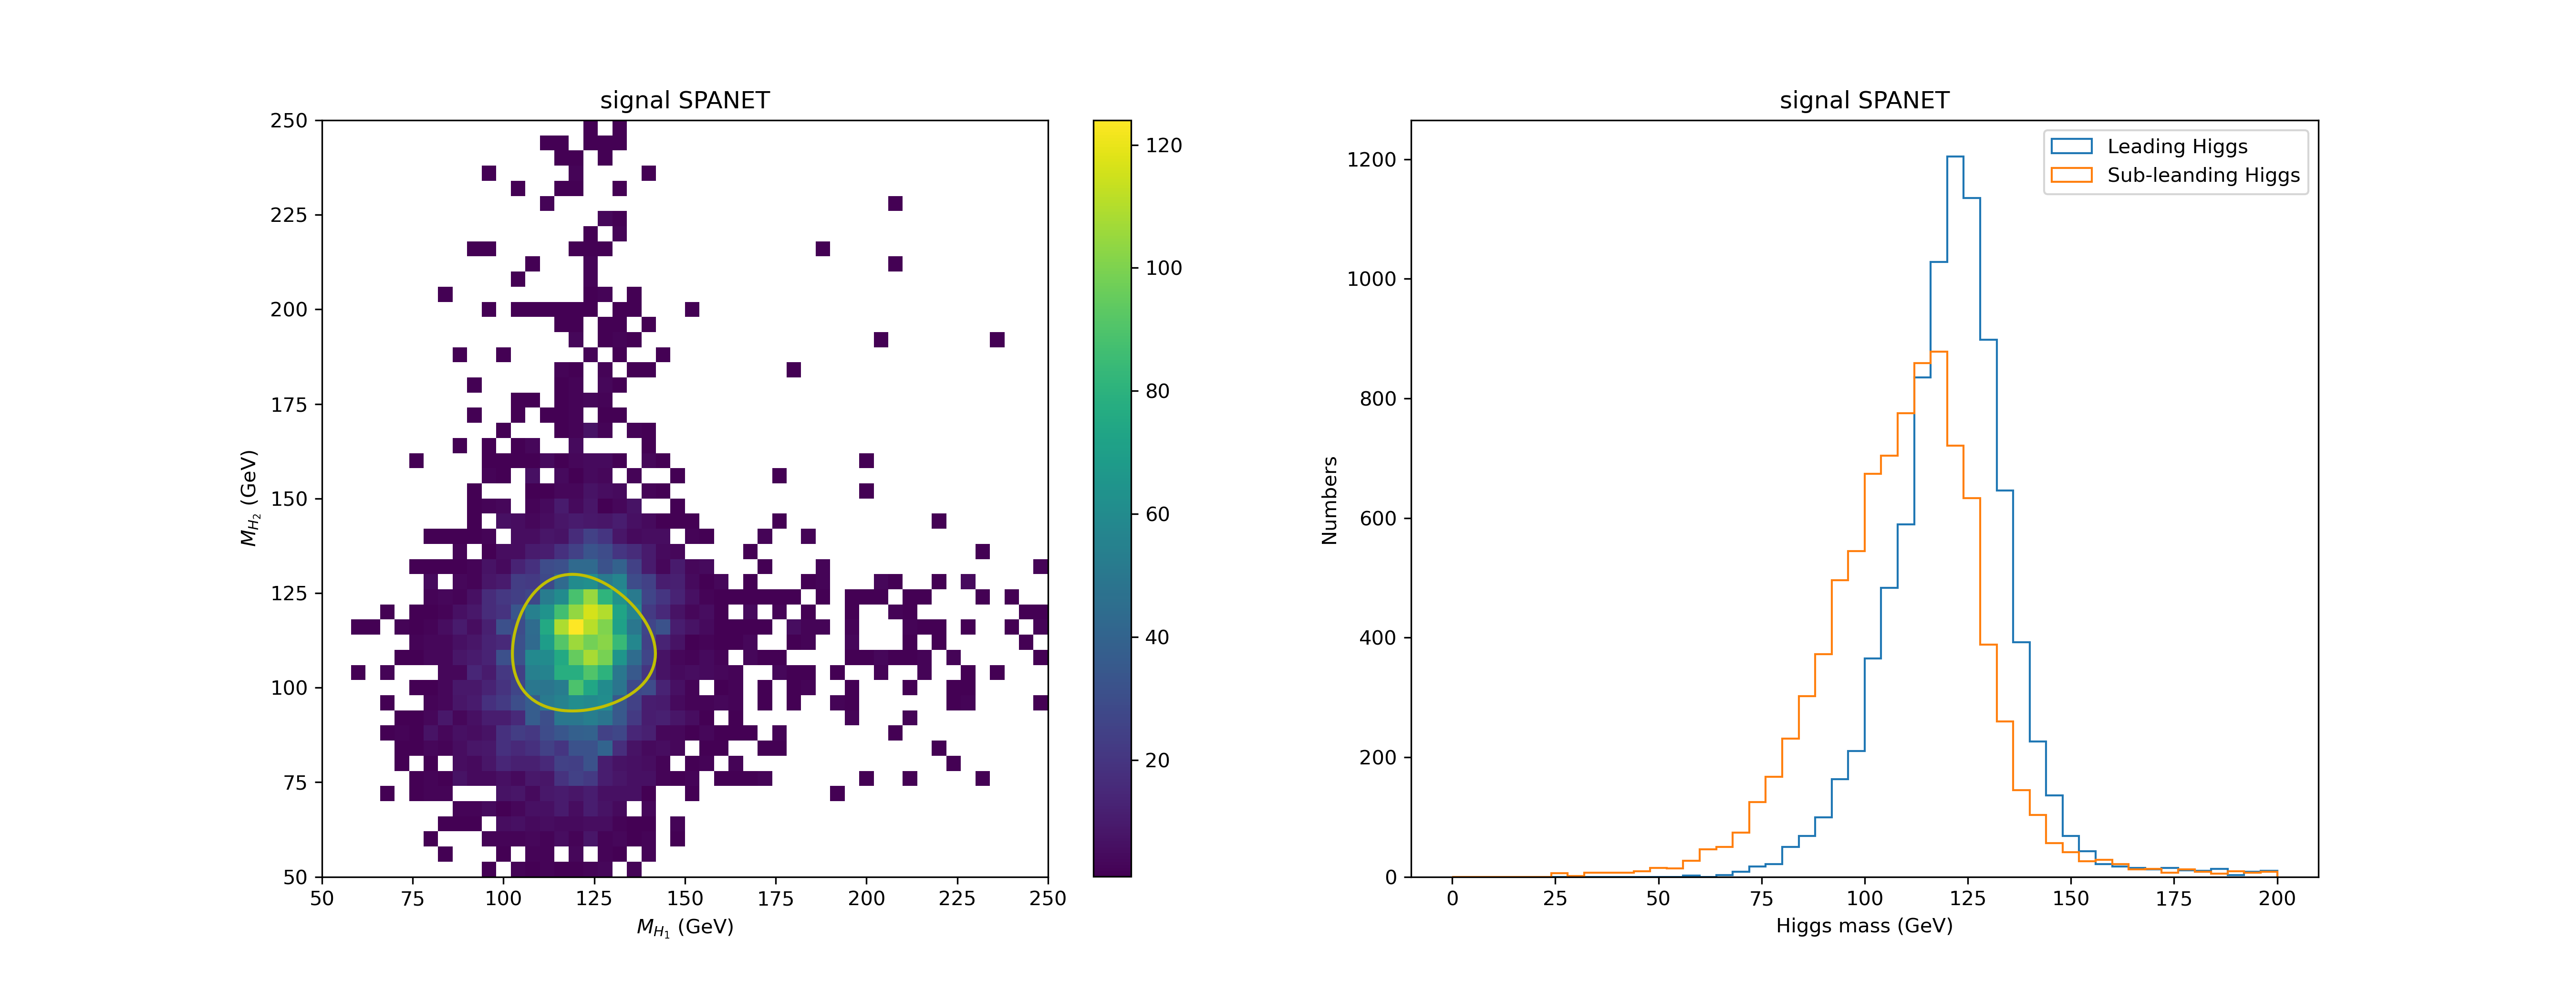
\includegraphics[width=0.97\textwidth]{Higgs_mass_old_SPANET_s.png}
		\caption{The mass plane and distribution of Higgs candidate for resonant signal events with different pairing methods. The top one is $\Delta R + \text{min-}D_{HH}$ pairing, the middle one is $\text{min-}\Delta R$ pairing, bottom one is SPA-NET pairing.}
		\label{fig:Higgs_mass_old_signal}
	\end{figure}

	\begin{figure}[htpb]
		\centering
		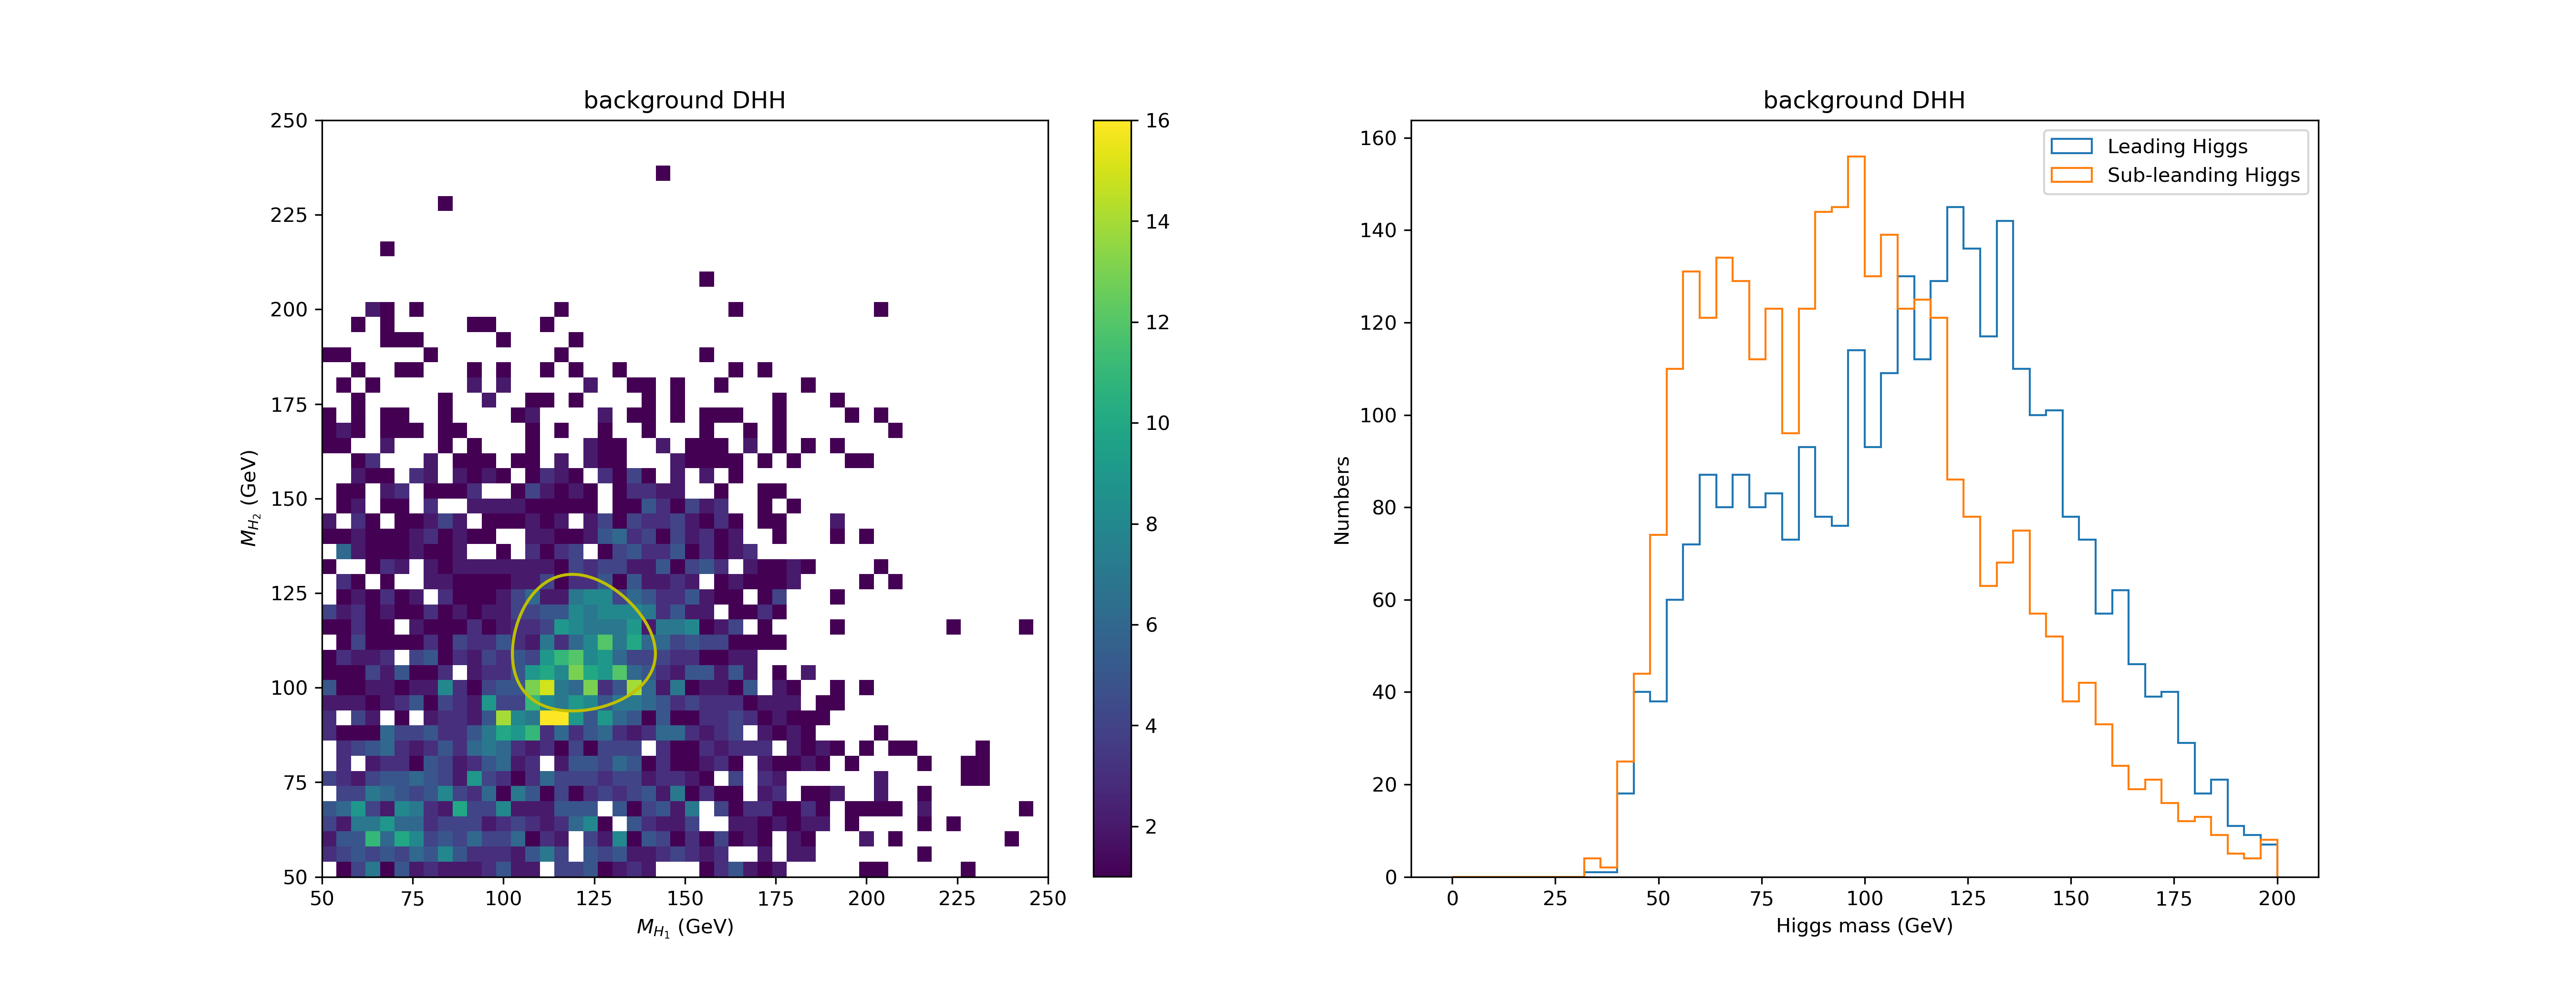
\includegraphics[width=0.97\textwidth]{Higgs_mass_old_DHH_4b.png}
		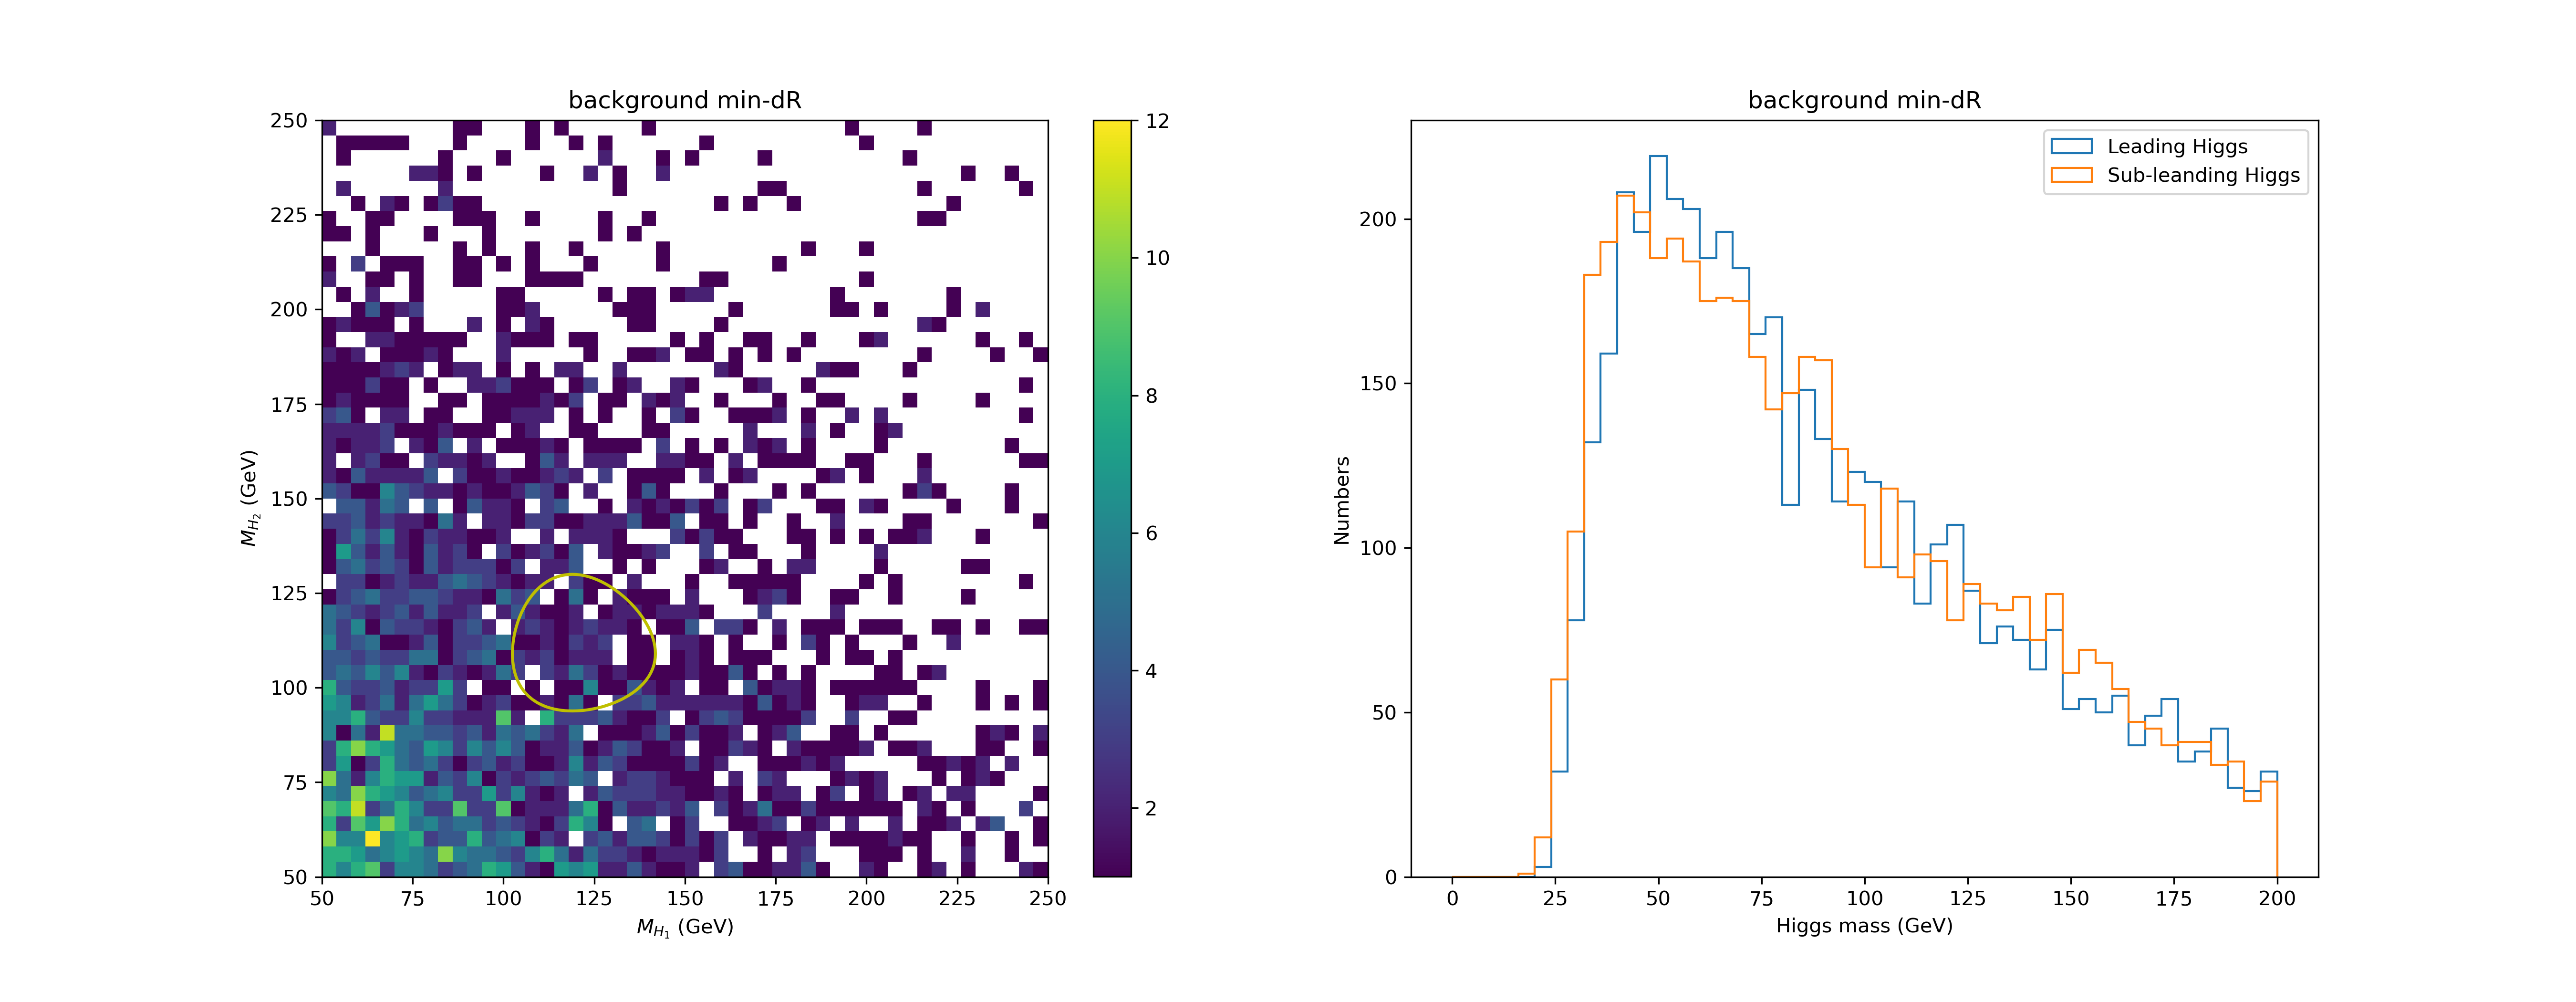
\includegraphics[width=0.97\textwidth]{Higgs_mass_old_mindR_4b.png}
		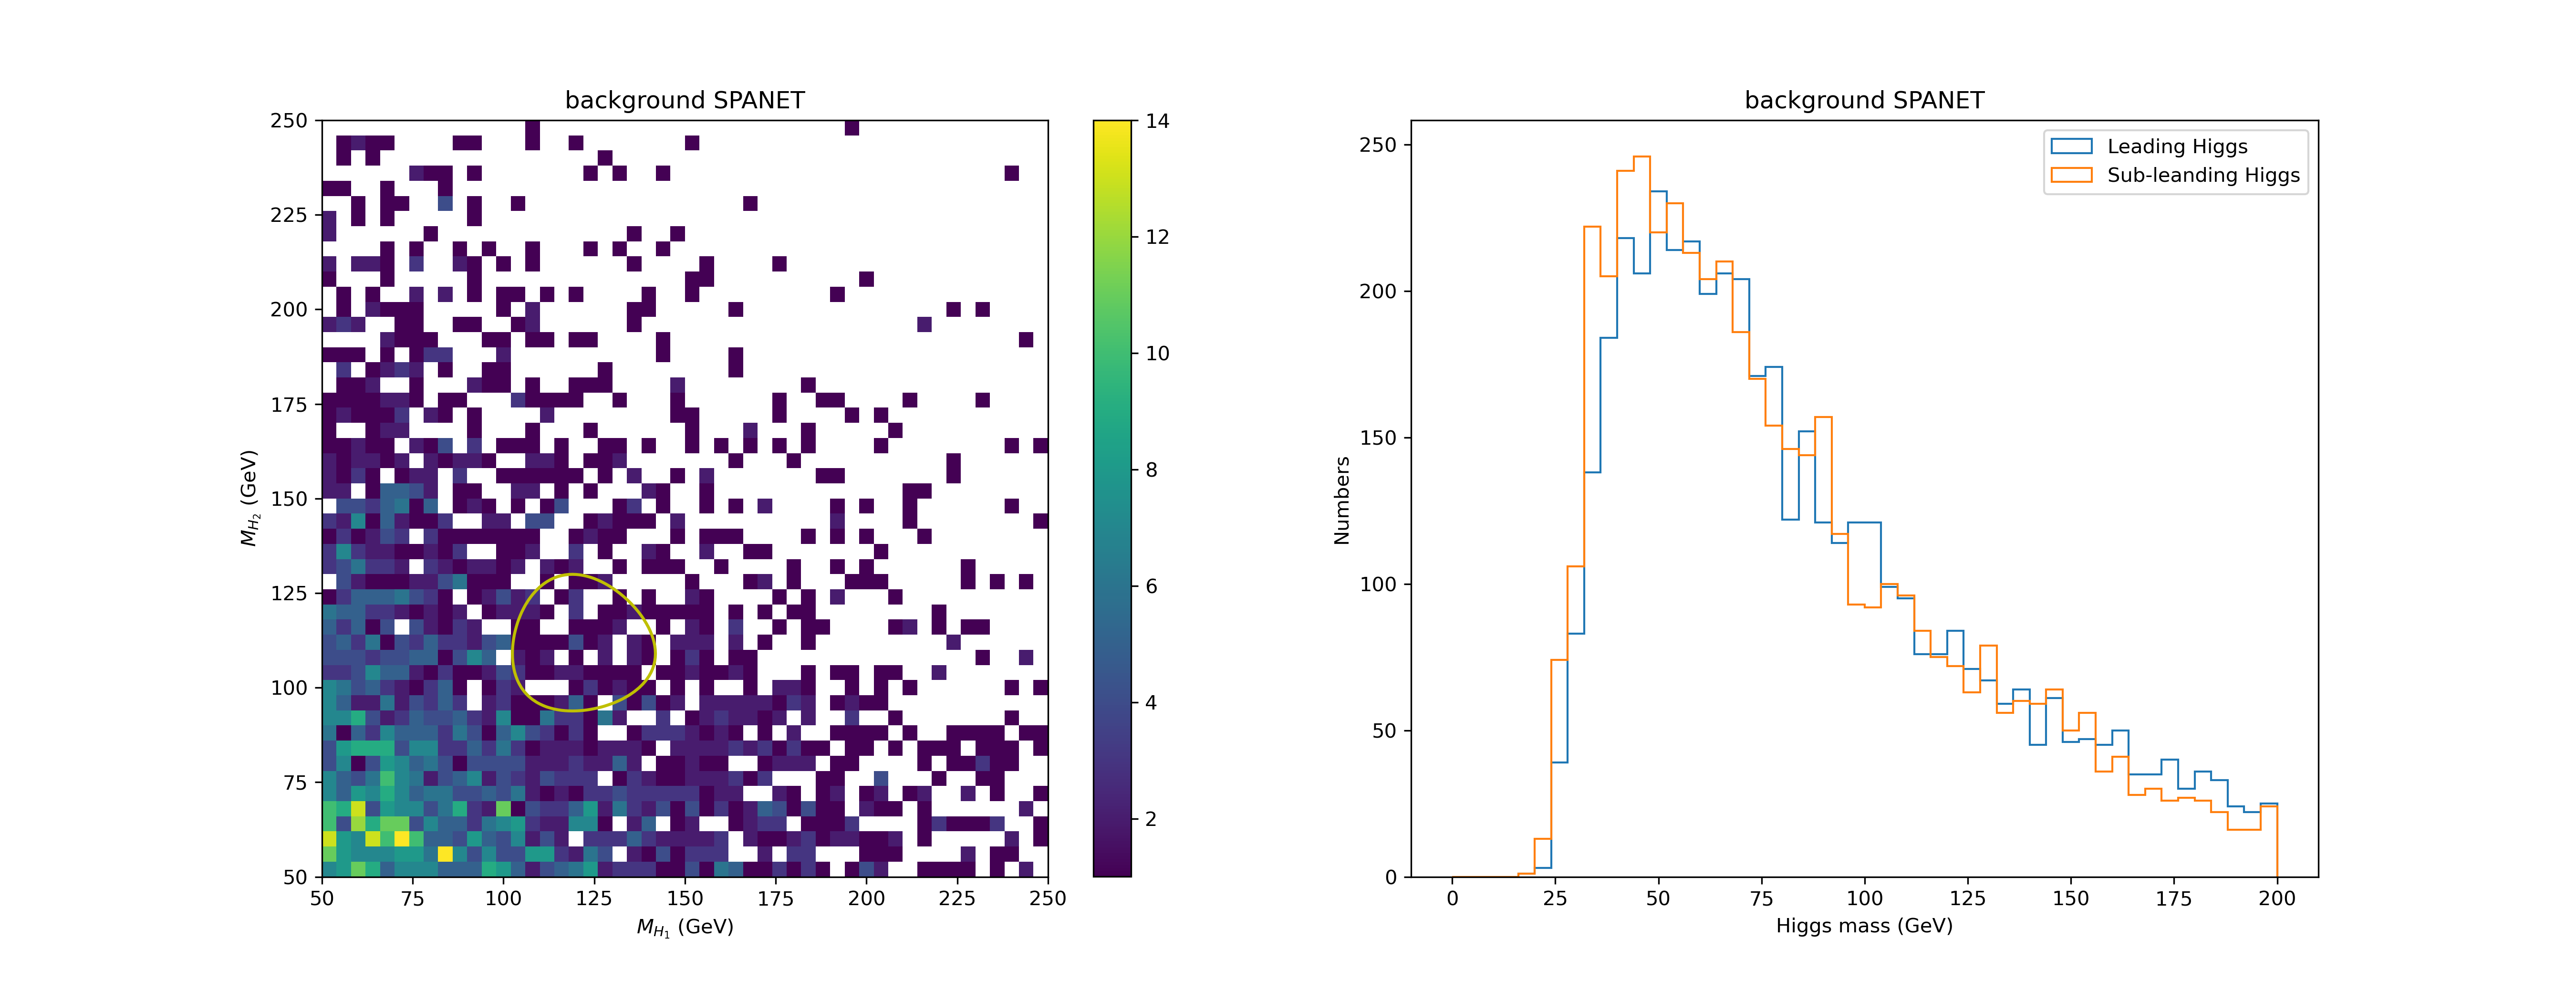
\includegraphics[width=0.97\textwidth]{Higgs_mass_old_SPANET_4b.png}
		\caption{The mass plane and distribution of Higgs candidate for background events with different pairing methods. The top one is $\Delta R + \text{min-}D_{HH}$ pairing, the middle one is $\text{min-}\Delta R$ pairing, bottom one is SPA-NET pairing.}
		\label{fig:Higgs_mass_old_background}
	\end{figure}

	The results of $S/\sqrt{B}$ are presented in Table \ref{tab:diHiggs_signal_background_analysis_ATLAS_1000GeV_DHH}, \ref{tab:diHiggs_signal_background_analysis_ATLAS_1000GeV_mindR}, \ref{tab:diHiggs_signal_background_analysis_ATLAS_1000GeV_SPANET}. Compared to the $\Delta R + \text{min-}D_{HH}$ pairing method, the $\text{min-}\Delta R$ and SPA-NET pairing method can reduce more background events, so they can improve the $S/\sqrt{B}$. The SPA-NET method has the best performance.
	\begin{table}[htpb]
		\centering
		\caption{The cross sections for the di-Higgs signal and background processes at different cuts. The pairing method is $\Delta R + \text{min-}D_{HH}$.}
		\label{tab:diHiggs_signal_background_analysis_ATLAS_1000GeV_DHH}
		\begin{tabular}{l|cc|c|c|c|c}
						 & \multicolumn{2}{c|}{Cross section (fb)} &          & $\mathcal{L} = 139 \text{ fb}^{-1}$ & $\mathcal{L} = 300 \text{ fb}^{-1}$ & $\mathcal{L} = 3000 \text{ fb}^{-1}$ \\
						 & Signal           & Background           & $S / B$  & $S/\sqrt{B}$                        & $S/\sqrt{B}$                        & $S/\sqrt{B}$                         \\ \hline
			No cut       & 0.644 & 6.29e+05 & 1.02e-06 & 0.0096 & 0.0141 & 0.0445 \\
			Four tag     & 0.081 & 6.06e+03 & 1.34e-05 & 0.0123 & 0.0180 & 0.0570 \\
			Delta R      & 0.070 & 3.17e+03 & 2.21e-05 & 0.0147 & 0.0215 & 0.0681 \\
			Higgs PT     & 0.058 & 2.68e+03 & 2.15e-05 & 0.0131 & 0.0193 & 0.0610 \\
			Higgs Eta    & 0.053 & 1.91e+03 & 2.78e-05 & 0.0143 & 0.0211 & 0.0666 \\
			Higgs signal & 0.029 & 2.97e+02 & 9.67e-05 & 0.0196 & 0.0288 & 0.0912 \\
			Top veto     & 0.027 & 1.77e+02 & 0.000155 & 0.0243 & 0.0357 & 0.1128
		\end{tabular}
	\end{table}
	\begin{table}[htpb]
		\centering
		\caption{The cross sections for the di-Higgs signal and background processes at different cuts. The pairing method is $\text{min-}\Delta R$.}
		\label{tab:diHiggs_signal_background_analysis_ATLAS_1000GeV_mindR}
		\begin{tabular}{l|cc|c|c|c|c}
						 & \multicolumn{2}{c|}{Cross section (fb)} &          & $\mathcal{L} = 139 \text{ fb}^{-1}$ & $\mathcal{L} = 300 \text{ fb}^{-1}$ & $\mathcal{L} = 3000 \text{ fb}^{-1}$ \\
						 & Signal           & Background           & $S / B$  & $S/\sqrt{B}$                        & $S/\sqrt{B}$                        & $S/\sqrt{B}$                         \\ \hline
			No cut       & 0.644 & 6.29e+05 & 1.02e-06 & 0.0096 & 0.0141 & 0.0445 \\
			Four tag     & 0.081 & 6.06e+03 & 1.34e-05 & 0.0123 & 0.0180 & 0.0570 \\
			Higgs PT     & 0.060 & 4.18e+03 & 1.44e-05 & 0.0110 & 0.0162 & 0.0511 \\
			Higgs Eta    & 0.056 & 3.15e+03 & 1.77e-05 & 0.0117 & 0.0172 & 0.0543 \\
			Higgs signal & 0.029 & 72.9     & 0.000393 & 0.0396 & 0.0582 & 0.1839 \\
			Top veto     & 0.027 & 59.1     & 0.000464 & 0.0420 & 0.0617 & 0.1952
		\end{tabular}
	\end{table}
	\begin{table}[htpb]
		\centering
		\caption{The cross sections for the di-Higgs signal and background processes at different cuts. The pairing method is SPA-NET.}
		\label{tab:diHiggs_signal_background_analysis_ATLAS_1000GeV_SPANET}
		\begin{tabular}{l|cc|c|c|c|c}
						 & \multicolumn{2}{c|}{Cross section (fb)} &          & $\mathcal{L} = 139 \text{ fb}^{-1}$ & $\mathcal{L} = 300 \text{ fb}^{-1}$ & $\mathcal{L} = 3000 \text{ fb}^{-1}$ \\
						 & Signal           & Background           & $S / B$  & $S/\sqrt{B}$                        & $S/\sqrt{B}$                        & $S/\sqrt{B}$                         \\ \hline
			No cut       & 0.644 & 6.29e+05 & 1.02e-06 & 0.0096 & 0.0141 & 0.0445 \\
			Four tag     & 0.081 & 6.06e+03 & 1.34e-05 & 0.0123 & 0.0180 & 0.0570 \\
			Higgs PT     & 0.063 & 4.22e+03 & 1.49e-05 & 0.0114 & 0.0168 & 0.0531 \\
			Higgs Eta    & 0.058 & 3.05e+03 & 1.9e-05  & 0.0124 & 0.0182 & 0.0574 \\
			Higgs signal & 0.030 & 47.1     & 0.000639 & 0.0517 & 0.0760 & 0.2403 \\
			Top veto     & 0.029 & 41.5     & 0.000692 & 0.0526 & 0.0772 & 0.2443
		\end{tabular}
	\end{table}

% section apply_the_min_delta_r_method_on_the_resonant_sample (end)		
\end{document} 
